\subsection{Estimation of the TVP-BVAR with SV using forgetting factors}
\label{app:est}
We consider the model
\begin{align}\label{eqn:Atvpvar1}
	y_t&=a_t+A_{1,t}\,y_{t-1}+\varepsilon_t,\\
	A_t&=\phi A_{t-1}+(1-\phi)\underline{A}_0+u_t,\label{eqn:Atvpvar2}
\end{align}
where $A_t=[a_t\,\,\, A_{1,t}]$ is an unknown state vector, $\underline{A}_0$ is some initial condition for each $t$ and also $A_0=\underline{A}_0$, $\varepsilon_t\stackrel{iid}{\sim}\No{0,\Sigma_t}$ with initial condition $\Sigma_0$, $u_t\stackrel{iid}{\sim}\No{0,\Omega_t}$ with initial condition $\Omega_0$ and $\varepsilon_t$ and $u_s$ are independent of each other for all $t$ and $s$. To estimate the mode, we run a Kalman filter for $t=1,\ldots,T$ as follows:\footnote{The algorithm is taken and amended from the technical appendix of the working paper version of \cite{koop2013}.}\\
\textbf{I. Prediction step:}
\begin{enumerate}
	%\item Set $\beta_{t|t-1}=\phi \beta_{t-1|t-1}+(1-\phi)\underline{\beta}_0$
	\item Set $A_{t|t-1}=\phi A_{t-1|t-1}+(1-\phi)\underline{A}_0$.
	%\item Estimate $\lambda_t=\lambda_{\text{min}}+(1-\lambda_{\text{min}})L^{f_t}$ with $f_t=-RNI(\tilde{\varepsilon}_{t-1}'\tilde{\varepsilon}_{t-1})$, where $RNI(\cdot)$ rounds to the nearest integer value.
	\item Set $P_{t|t-1}=\frac{1}{\lambda}P_{t-1|t-1}$\\
	where for $t=1$ we set $A_{0|0}=\underline{A}_0$ and $P_{0|0}=\underline{P}_0$.
\end{enumerate}
\textbf{II. Update step:}
\begin{enumerate}
	\item Calculate $\tilde{\varepsilon}_t=y_t-a_{t|t-1}+A_{t|t-1}\,y_{t-1}$.
	\item Calculate $\hat{\Sigma}_t=\kappa\hat{\Sigma}_{t-1}+(1-\kappa)\tilde{\varepsilon}_t'\tilde{\varepsilon}_t$ with $\hat{\Sigma}_1=\kappa\Sigma_0$.
	%\item Estimate $\beta_{t|t}=\beta_{t|t-1}+P_{t|t-1}[1\,\, y_{t-1}]'\left(\hat{\Sigma}_t+[1\,\, y_{t-1}]P_{t|t-1}[1 y_{t-1}]'\right)^{-1}\tilde{\epsilon}_t$\
	\item Estimate $A_{t|t}=A_{t|t-1}+P_{t|t-1}[1 y_{t-1}]'\left(\hat{\Sigma}_t+[1 y_{t-1}]P_{t|t-1}[1 y_{t-1}]'\right)^{-1}\tilde{\epsilon}_t$.
	\item Calculate $P_{t|t}=P_{t|t-1}+P_{t|t-1}[1 y_{t-1}]'\left(\hat{\Sigma}_t+[1 y_{t-1}]P_{t|t-1}[1 y_{t-1}]'\right)^{-1}P_{t|t-1}$.
\end{enumerate}
The one-step ahead predictive density of the VAR model is then analytically available from the Kalman filter as
\begin{equation}
p(y_t|y^t)\sim\No{[1\,\, y_{t+1}]A_{t+1|t},\hat{\Sigma}_{t+1}+[1\,\, y_{t+1}]A_{t+1|t}[1\,\, y_{t+1}]'}.
\end{equation}

\clearpage
\newpage

\subsection{Figures}

\begin{figure}[ht!]
	\centering
	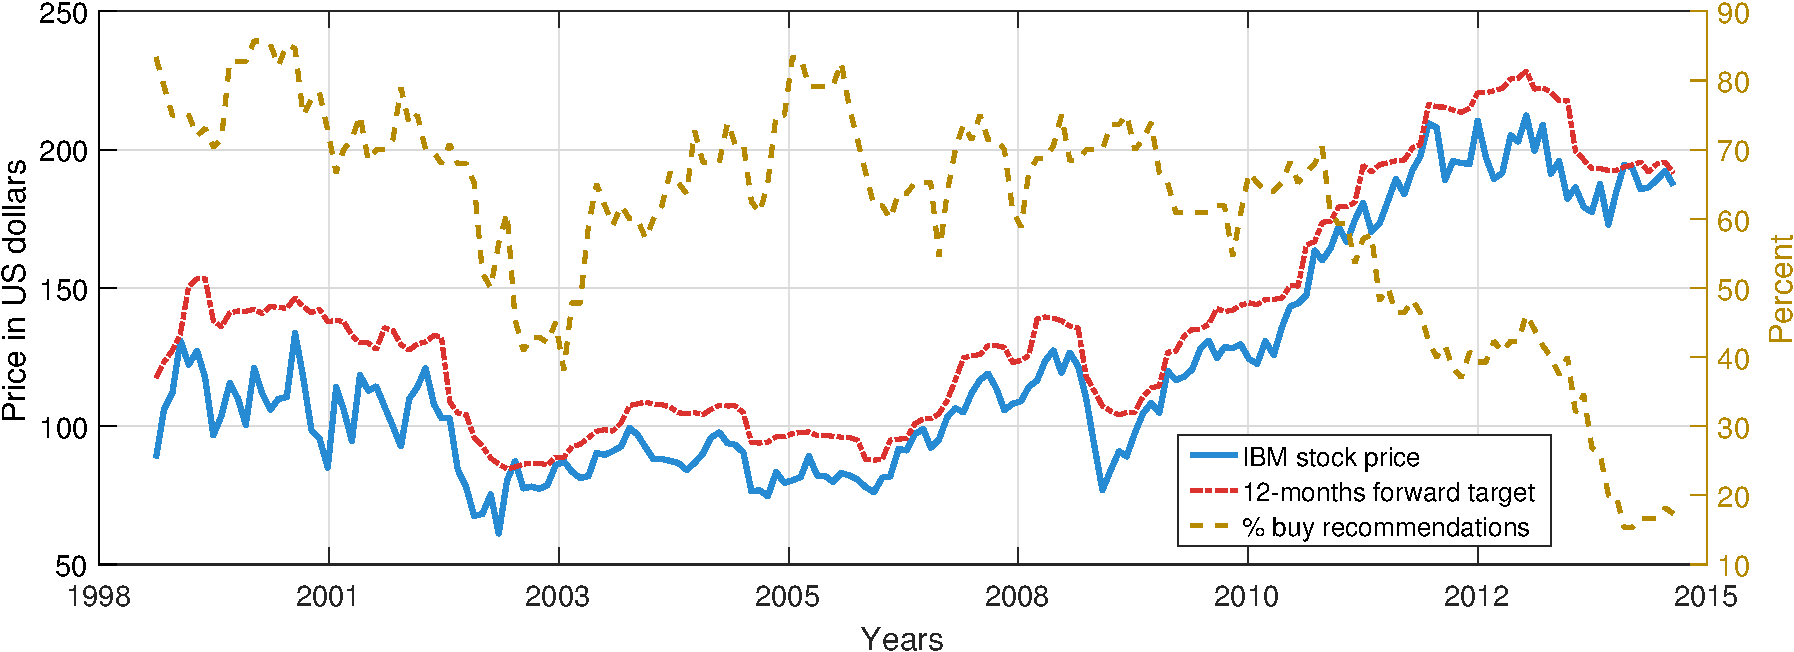
\includegraphics[width=1\linewidth]{../plots/IBM_price_plot}
	\caption[Spot price, 12 months forward target price and percentage of buy recommendations of the IBM stock (monthly data) between 1999 and 2015]{The figure shows IBM spot price, the mean 12 months forward target price and the percentage of buy recommendations from all recommendations (buy, sell, hold) of the IBM stock between 1999 and 2015.}
	\label{fig:ibmpriceplot}
\end{figure}

\begin{figure}[ht!]
	\centering
	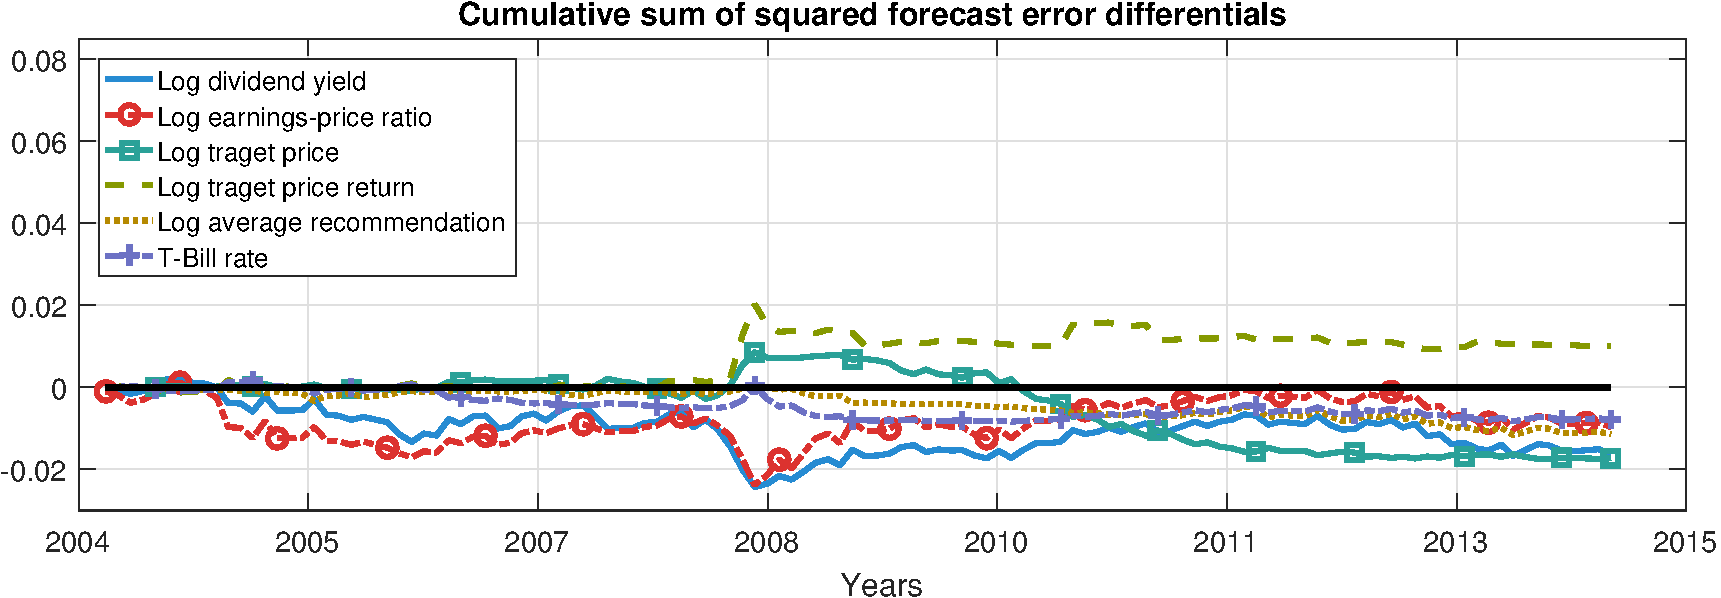
\includegraphics[width=1\linewidth]{../plots/IBM_CSSED_plot}
	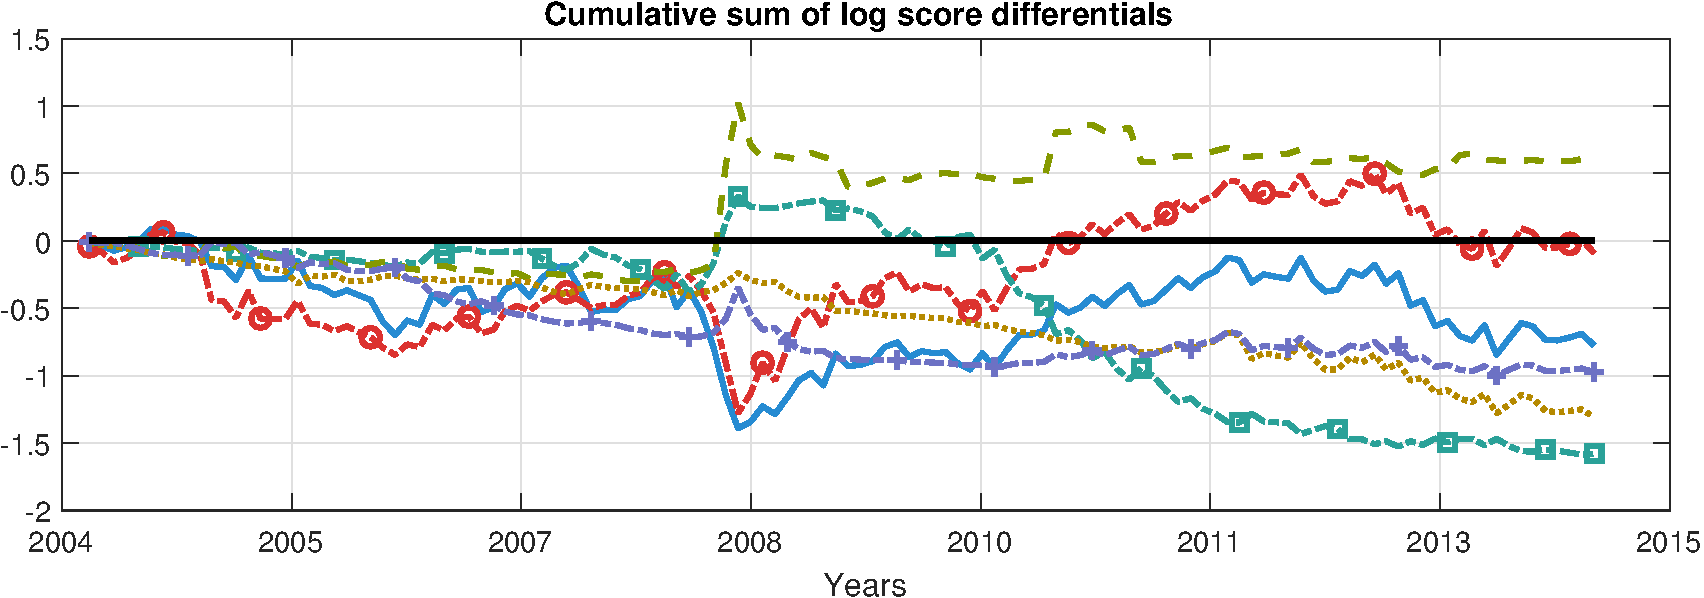
\includegraphics[width=1\linewidth]{../plots/IBM_CLSD_plot}
	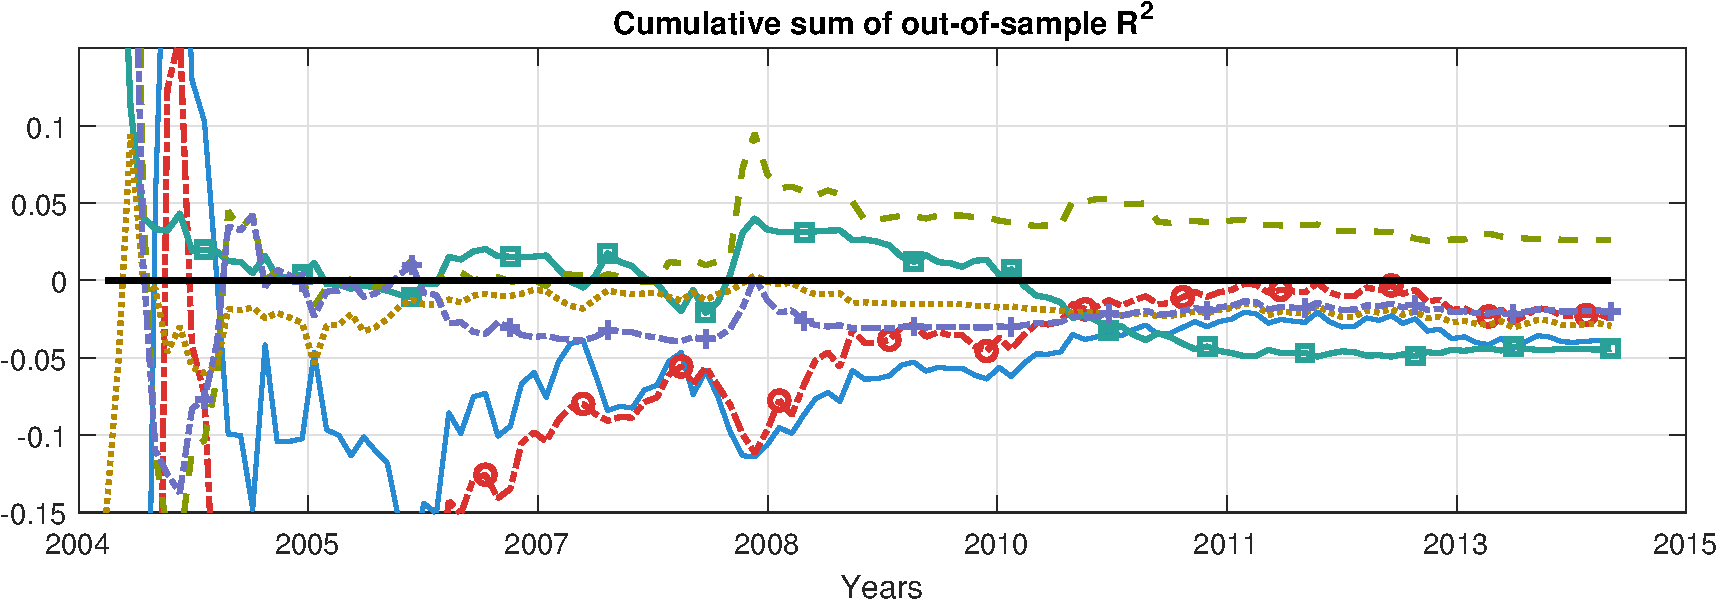
\includegraphics[width=1\linewidth]{../plots/IBM_R2_plot}
	\caption[Out-of-sample forecast performance results for different univariate models for the IBM stock for 2004 to 2015]{The figure provides out-of-sample forecast performance results for different univariate models for the IBM stock for 2004 to 2015. The top panel shows the cumulative sum of squared forecast errors of the benchmark mean model model minus the sum of squared forecast errors for six univariate models with different regressors, i.e. for model $m$ this is $\text{CSSED}_{m,t}=\sum_{i=S+1}^{t}\left(e_{0,i}^2-e_{m,i}^2\right)$. Each model is estimated from a linear regression of monthly excess returns on an intercept and a lagged predictor variable, i.e. $r_t=\alpha+\beta x_{t-1}+\varepsilon_t$. The middle panel shows the cumulative sum of log predictive scores of the six models minus the sum of log predictive scores of the benchmark mean model. The bottom panel shows the cumulative sum of out-of-sample $\text{R}^2$ values of each of the six univariate models. For all three panels it holds that values above zero indicate that a given predictor has better forecast performance than the benchmark model, while negative values suggest the opposite.}
	\label{fig:ibmclsdplot}
\end{figure}



\begin{figure}
	\centering
	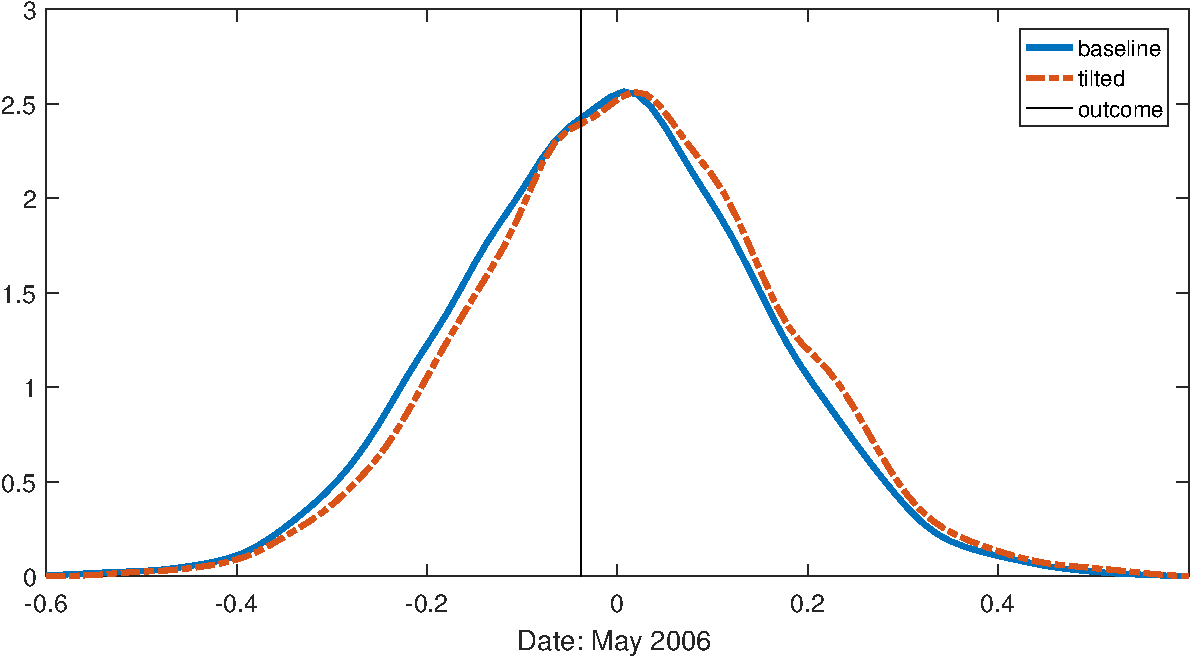
\includegraphics[width=0.49\linewidth]{../plots/IBM_density_m1}
	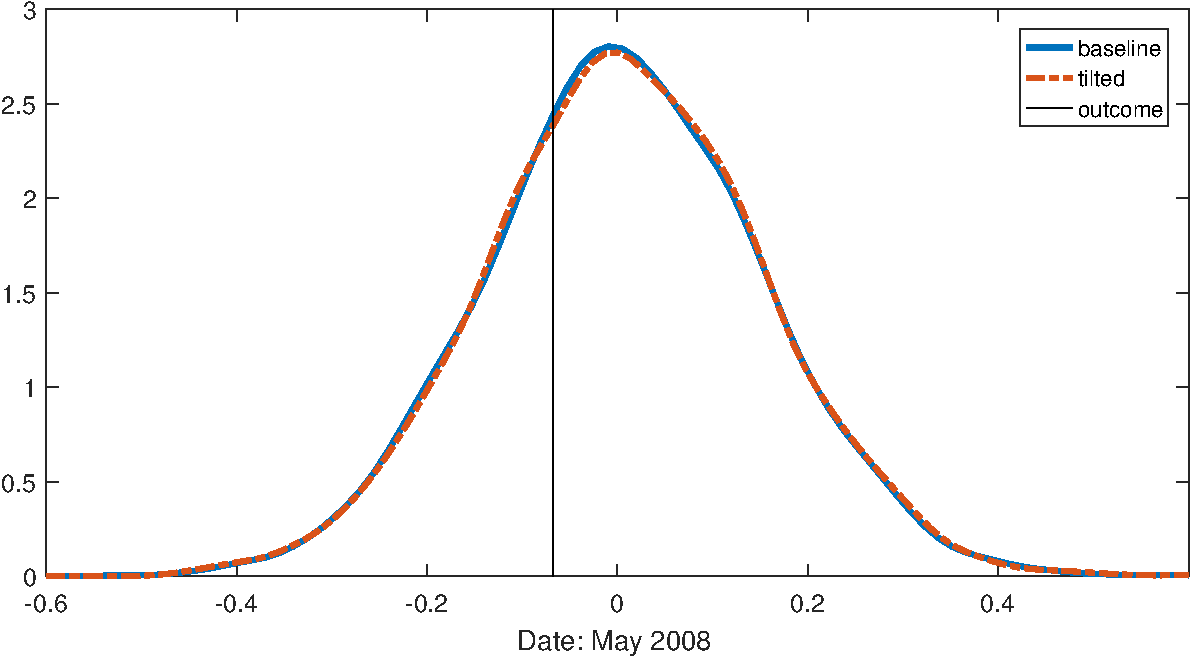
\includegraphics[width=0.49\linewidth]{../plots/IBM_density_m2}\\
	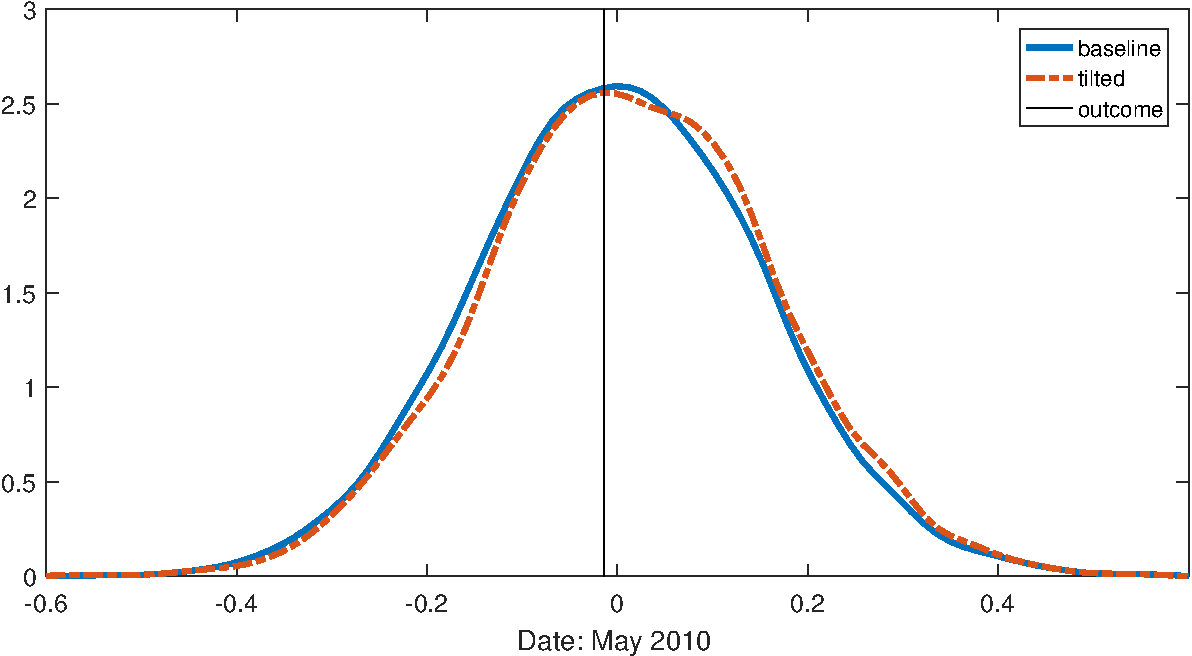
\includegraphics[width=0.49\linewidth]{../plots/IBM_density_m3}
	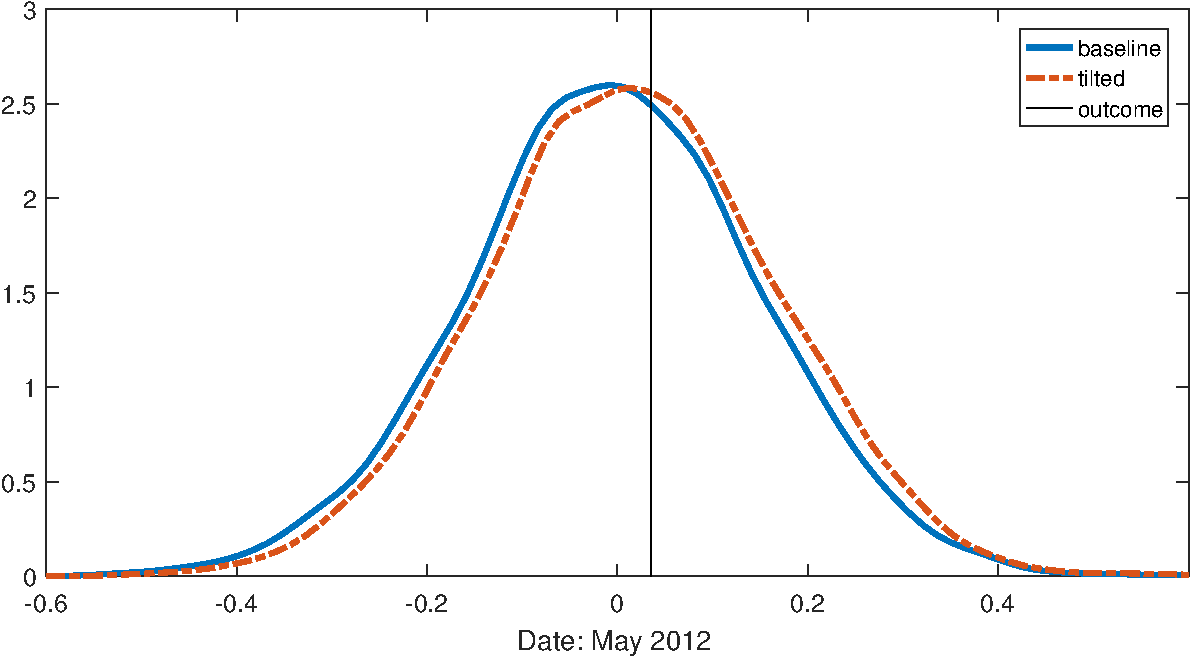
\includegraphics[width=0.49\linewidth]{../plots/IBM_density_m4}
	\caption[Kernel estimates of predictive density of the IBM returns from the TVPVAR(1) with dynamic model averaging and tilting towards the mean of monthly target price implied expected returns]{The figure shows the kernel of the predictive density of the IBM returns from the TVPVAR(1) model with dynamic model averaging and mean tilting towards the target price implied expected return at different times. The black horizontal line indicates the actual outcome return)}
	\label{fig:ibmdensitym}
\end{figure}

\begin{figure}
	\centering
	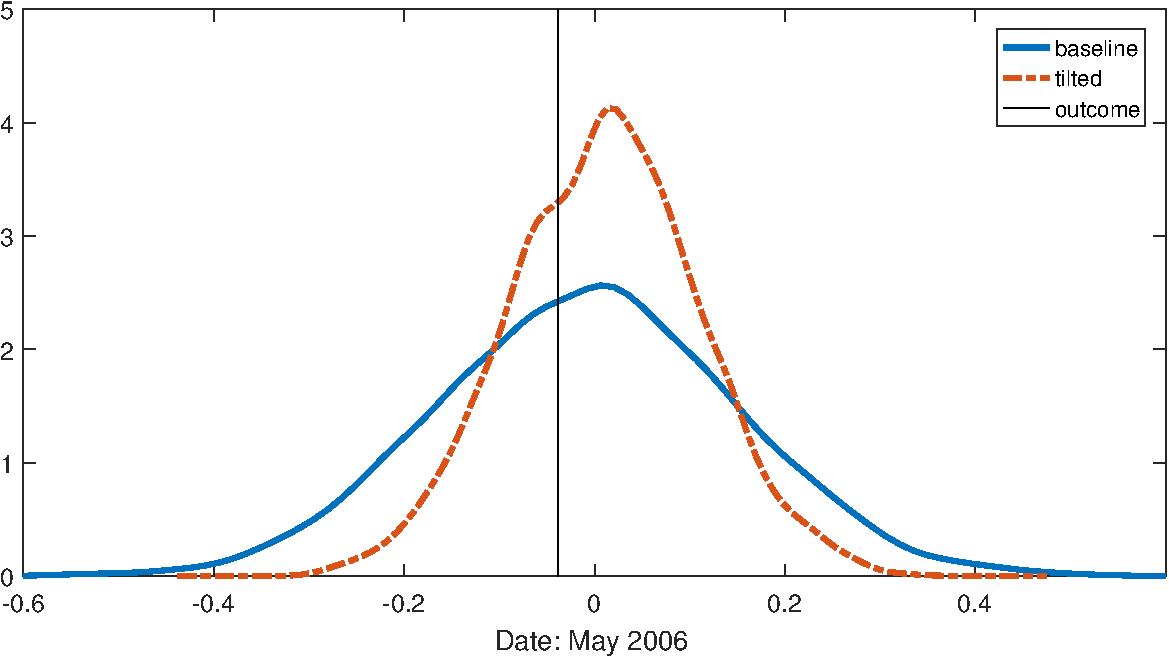
\includegraphics[width=0.49\linewidth]{../plots/IBM_density_mv1}
	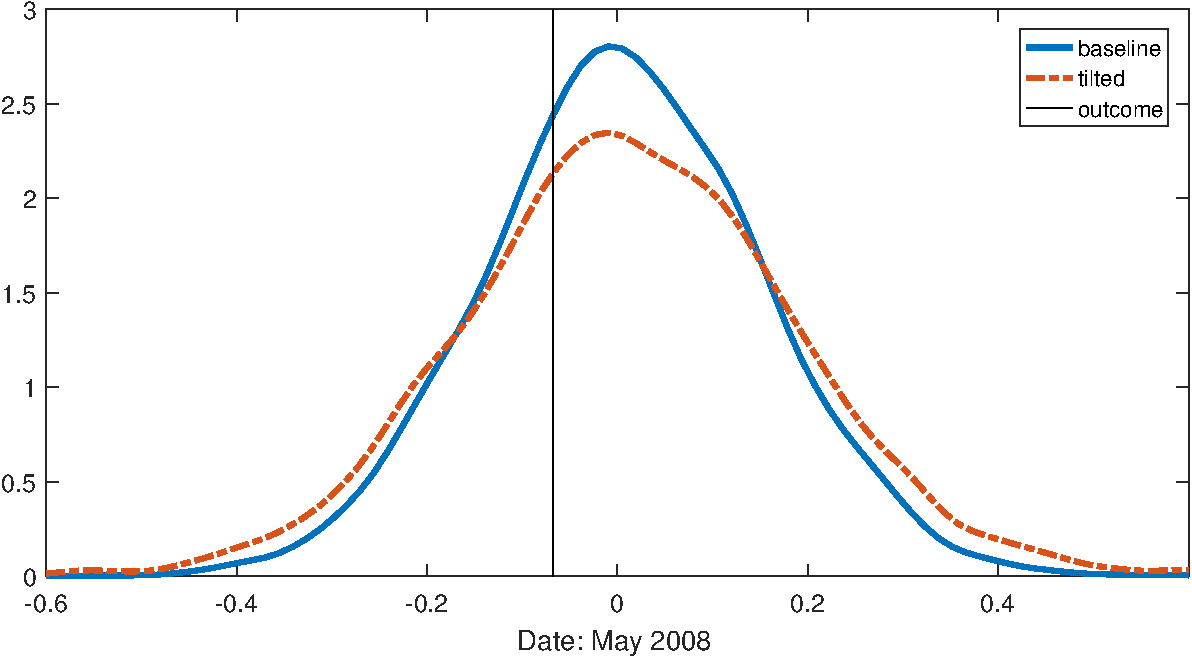
\includegraphics[width=0.49\linewidth]{../plots/IBM_density_mv2}\\
	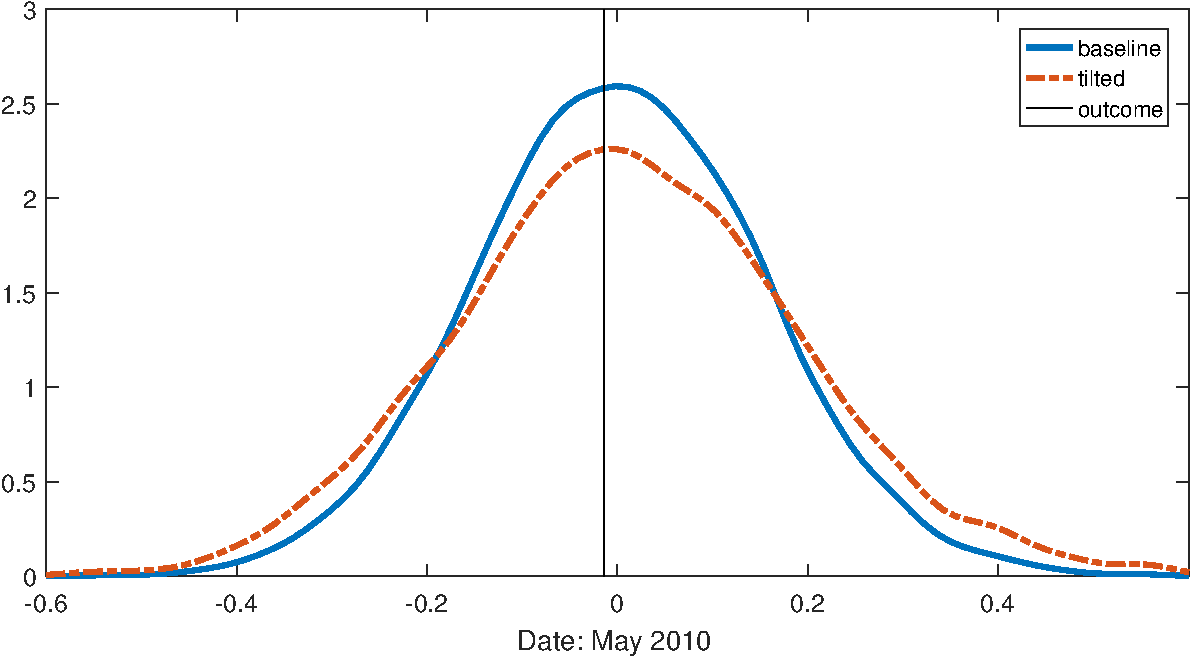
\includegraphics[width=0.49\linewidth]{../plots/IBM_density_mv3}
	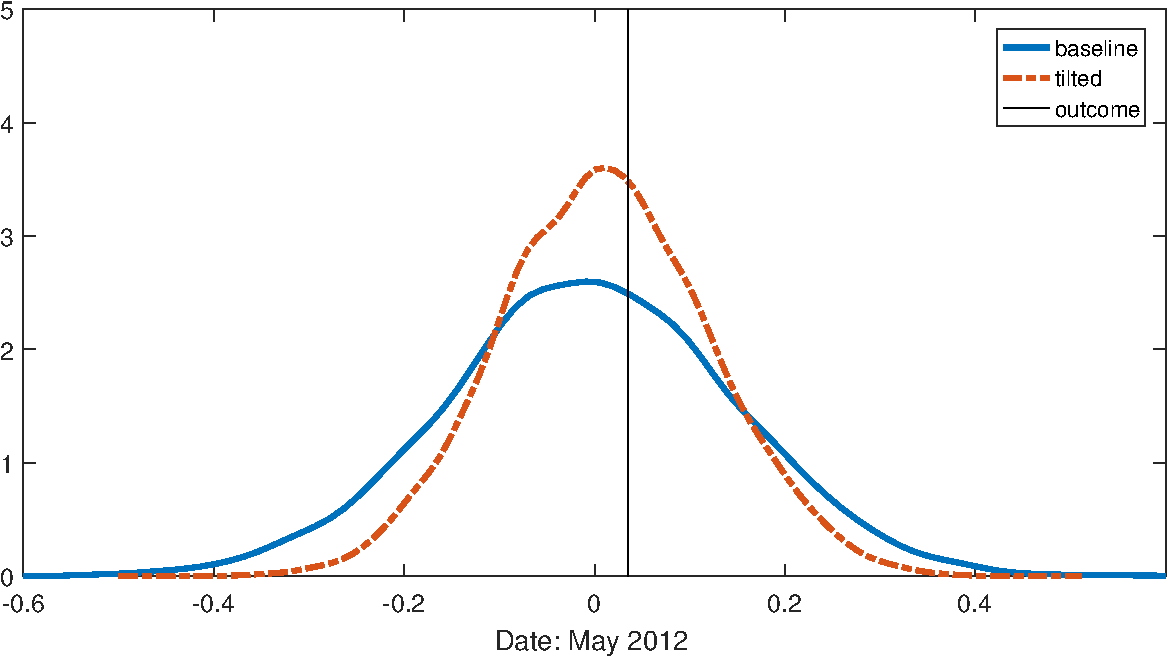
\includegraphics[width=0.49\linewidth]{../plots/IBM_density_mv4}
	\caption[Kernel estimates of predictive density of the IBM returns from the TVPVAR(1) with dynamic model averaging and tilting towards the mean and variance of monthly target price implied expected returns]{The figure shows the kernel of the predictive density of the IBM returns from the TVPVAR(1) model with dynamic model averaging with tilting towards the mean and variance of the target price implied expected returns at different times. The black horizontal line indicates the actual outcome return)}
	\label{fig:ibmdensitymv}
\end{figure}

\newpage\clearpage

\subsection{Tables}
\begin{table}[h!]
\fontsize{11}{18}\selectfont{
\begin{center}
\caption{Relative root mean squared errors between forecasted and observed spot prices for 20 Dow Jones constituents (sample: 1999 - 2015) }
\label{tab:rmsfe}
\vspace{-0.2cm}
\begin{tabularx}{1\textwidth}{@{}X@{\hspace{0.25cm}}c@{\hspace{0.25cm}}c@{\hspace{0.25cm}}c@{\hspace{0.25cm}}c@{\hspace{0.25cm}}c@{\hspace{0.25cm}}c@{\hspace{0.25cm}}c@{\hspace{0.25cm}}c@{\hspace{0.25cm}}c@{\hspace{0.25cm}}c@{}}
\toprule\toprule
 Stock  & AA	 & AAPL	 & AIG	 & AXP	 & BA	 & CAT	 & KO	 & DD	 & GE	 & HD	\\
\midrule
 rRMSFE  & $1.33^{**}$	 & \textbf{0.74}	 & $1.45^{***}$	 & \textbf{0.93}	 & \textbf{0.87}	 & \textbf{0.96}	 & 1.09	 & $1.24^{**}$	 & 1.23	 & \textbf{0.83}	\\
\midrule
\midrule
 Stock  & INTC	 & IBM	 & JNJ	 & MCD	 & MRK	 & MSFT	 & PG	 & UTX	 & WMT	 & DIS	\\
\midrule
 rRMSFE  & 1.36	 & \textbf{0.94}	 & \textbf{0.85}	 & $\mathbf{0.69^{***}}$	 & $1.25^{*}$	 & $1.65^{***}$	 & 1.01	 & \textbf{0.82}	 & 1.24	 & \textbf{0.84}	\\
\bottomrule\bottomrule
\end{tabularx}
\vspace{0.2cm}
\caption*{\footnotesize \textit{Note:} The table displays relative root mean squared errors between observed spot price twelve months ahead and the mean 12-month forward target price as well as the two year historical average for 20 Dow Jones constituents between 1999 and 2015. Values lower than one indicate that the target price generates superior forecast performance. For each stock, we test whether the target price forecast has lower MSFE than the average price forecast by the test proposed by \citet{giacomini2006}. One/two/three asterisks denote rejection of the null hypothesis of equal predictive ability at the ten/five/one percent test level.}
\end{center}}
\end{table}
\begin{table}[h!]
\fontsize{11}{18}\selectfont{
\begin{center}
\caption{Descriptive statistics on the returns, target prices and recommendations for 20 Dow Jones constituents (sample: 1999 - 2015) }
\label{tab:summary}
\vspace{-0.2cm}
\begin{tabularx}{1\textwidth}{@{}X@{\hspace{0.25cm}}c@{\hspace{0.25cm}}c@{\hspace{0.25cm}}c@{\hspace{0.25cm}}c@{\hspace{0.25cm}}c@{\hspace{0.25cm}}c@{\hspace{0.25cm}}c@{\hspace{0.25cm}}c@{\hspace{0.25cm}}c@{\hspace{0.25cm}}c@{}}
\toprule\toprule
 Stock  & AA	 & AAPL	 & AIG	 & AXP	 & BA	 & CAT	 & KO	 & DD	 & GE	 & HD	\\
\midrule
 Mean log ret  & -0.52	 & 2.01	 & -1.79	 & 0.26	 & 0.41	 & 0.43	 & -0.05	 & -0.18	 & -0.35	 & 0.27	\\
 Std log return  & 12.00	 & 14.13	 & 21.28	 & 9.52	 & 8.95	 & 10.13	 & 6.03	 & 8.27	 & 8.74	 & 8.22	\\
\midrule
 \# price tragets  & 14.38	 & 25.19	 & 13.17	 & 16.61	 & 16.18	 & 13.99	 & 13.11	 & 11.81	 & 13.33	 & 18.39	\\
 Mean exp ret  & 1.44	 & 1.44	 & 2.52	 & 1.12	 & 1.03	 & 1.08	 & 0.95	 & 1.30	 & 1.31	 & 1.10	\\
 Std exp ret  & 10.72	 & 7.49	 & 25.95	 & 6.08	 & 7.04	 & 7.20	 & 4.57	 & 5.79	 & 6.07	 & 6.37	\\
\midrule
 \# RECs  & 18.40	 & 32.33	 & 20.19	 & 21.36	 & 23.18	 & 20.09	 & 17.73	 & 16.48	 & 17.07	 & 25.76	\\
 Mean RECs  & 2.35	 & 2.13	 & 2.19	 & 2.36	 & 2.26	 & 2.29	 & 2.11	 & 2.40	 & 2.02	 & 2.11	\\
 Std RECs  & 0.38	 & 0.38	 & 0.58	 & 0.35	 & 0.38	 & 0.25	 & 0.25	 & 0.28	 & 0.34	 & 0.25	\\
\midrule
\midrule
 Stock  & INTC	 & IBM	 & JNJ	 & MCD	 & MRK	 & MSFT	 & PG	 & UTX	 & WMT	 & DIS	\\
\midrule
 Mean log ret  & -0.13	 & 0.14	 & 0.24	 & 0.27	 & -0.24	 & -0.09	 & 0.14	 & 0.39	 & 0.10	 & 0.40	\\
 Std log return  & 11.57	 & 7.76	 & 5.26	 & 6.54	 & 7.88	 & 8.90	 & 5.78	 & 7.25	 & 5.76	 & 7.91	\\
\midrule
 \# price tragets  & 28.66	 & 17.20	 & 14.66	 & 14.92	 & 15.53	 & 23.65	 & 13.34	 & 14.89	 & 17.98	 & 20.19	\\
 Mean exp ret  & 1.34	 & 0.95	 & 0.71	 & 1.10	 & 0.97	 & 1.53	 & 0.86	 & 0.95	 & 1.06	 & 1.26	\\
 Std exp ret  & 7.91	 & 5.29	 & 3.68	 & 5.40	 & 5.91	 & 6.91	 & 3.80	 & 4.52	 & 4.16	 & 6.62	\\
\midrule
 \# RECs  & 39.53	 & 23.10	 & 23.78	 & 20.60	 & 24.28	 & 32.73	 & 18.77	 & 19.98	 & 26.02	 & 27.22	\\
 Mean RECs  & 2.18	 & 2.18	 & 2.10	 & 2.16	 & 2.42	 & 1.91	 & 2.09	 & 1.95	 & 2.05	 & 2.29	\\
 Std RECs  & 0.29	 & 0.26	 & 0.25	 & 0.26	 & 0.36	 & 0.26	 & 0.21	 & 0.24	 & 0.25	 & 0.25	\\
\bottomrule\bottomrule
\end{tabularx}
\vspace{0.2cm}
\caption*{\footnotesize \textit{Note:} The table reports descriptive statistics on the returns, expected target returns and recommendations  for 20 Dow Jones constituents. It reports the mean and standard deviation of the logarithmic monthly returns, the mean number of available target prices, the mean and variance of the monthly forward target price implied expected return, i.e. simple returns between the spot and the twelve month forward target price at each point $t$ divided by 12, constructed from individual analyst data, the mean number of recommendations as well as the mean and standard deviation of the recommendations based on the 1 (strong buy) to 5 (strong sell) scale. Mean returns and standard deviations are multiplied by 100. Target prices and recommendations are obtained from I/B/E/S Datastream.}
\end{center}}
\end{table} 

%
%\begin{table}[h!]
\fontsize{11}{15}\selectfont{
\begin{center}
\caption{Forecast performance in terms of out-of-sample R$^2$ for 20 Dow Jones constituents (sample: 2004 - 2015) using a Bayesian VAR(1)}
\label{tab:mRsquard_BVAR}
\vspace{-0.2cm}
\begin{tabularx}{1\textwidth}{@{}X@{\hspace{0.2cm}}l@{\hspace{0.2cm}}l@{\hspace{0.2cm}}l@{\hspace{0.2cm}}l@{\hspace{0.2cm}}l@{\hspace{0.2cm}}l@{\hspace{0.2cm}}l@{\hspace{0.2cm}}l@{\hspace{0.2cm}}l@{\hspace{0.2cm}}l@{}}
\toprule\toprule
 Stock  & AA	 & AAPL	 & AIG	 & AXP	 & BA	 & CAT	 & KO	 & DD	 & GE	 & HD	\\
\midrule
 Log DY  & -6.90	 & \textbf{0.20}	 & -3.46	 & -0.68	 & -1.24	 & -0.51	 & -0.04	 & -0.20	 & -0.44	 & -0.13	\\
 Log EPR  & -1.97	 & \textbf{0.13}	 & -0.82	 & -0.30	 & -5.98	 & -0.06	 & -0.22	 & -0.16	 & -0.32	 & -0.62	\\
 Log DPR  & -0.13	 & -0.04	 & -0.05	 & -0.09	 & -1.09	 & \textbf{0.13}	 & -0.10	 & \textbf{0.25}	 & -0.13	 & -0.18	\\
 BMR  & -0.15	 & \textbf{0.21}	 & -1.18	 & -0.14	 & -0.13	 & -0.13	 & -0.73	 & -0.24	 & \textbf{0.00}	 & -0.06	\\
\midrule
 3M Tbill rate  & -0.10	 & \textbf{0.09}	 & -0.07	 & \textbf{0.33}	 & \textbf{0.06}	 & -0.18	 & -0.36	 & -0.28	 & -0.11	 & -0.17	\\
 Market return  & -0.09	 & \textbf{0.22}	 & -0.02	 & -0.06	 & -0.05	 & -0.12	 & -0.09	 & -0.21	 & -0.11	 & -0.57	\\
 LT yield  & -0.22	 & \textbf{0.03}	 & \textbf{0.24}	 & -0.15	 & -0.35	 & -0.27	 & -0.42	 & -0.28	 & -0.09	 & -0.29	\\
 CPI inflation  & -0.15	 & \textbf{0.18}	 & -0.10	 & -0.14	 & -0.13	 & -0.19	 & -0.30	 & -0.19	 & -0.20	 & \textbf{0.14}	\\
\midrule
 Log TPR  & -0.05	 & -0.16	 & -0.58	 & -0.45	 & -0.10	 & -0.13	 & -0.30	 & -0.17	 & -0.50	 & -0.20	\\
 Log TPV  & -0.24	 & \textbf{0.15}	 & -0.12	 & -0.17	 & -0.12	 & -0.53	 & -0.16	 & -0.19	 & -0.28	 & \textbf{0.28}	\\
 Log REC  & -0.54	 & \textbf{0.01}	 & -0.08	 & -0.48	 & -1.10	 & -0.31	 & -0.52	 & -0.72	 & -0.22	 & -0.08	\\
 Log REC return  & $\mathbf{8.06^{***}}$	 & -0.36	 & -0.09	 & \textbf{0.09}	 & -0.32	 & -0.01	 & $\mathbf{8.06^{***}}$	 & $\mathbf{8.06^{***}}$	 & -0.11	 & -0.02	\\
\midrule
\midrule
 Stock  & INTC	 & IBM	 & JNJ	 & MCD	 & MRK	 & MSFT	 & PG	 & UTX	 & WMT	 & DIS	\\
\midrule
 Log DY  & -0.35	 & -0.20	 & -0.46	 & -0.39	 & -0.31	 & -0.22	 & -0.43	 & -0.06	 & -0.23	 & -0.01	\\
 Log EPR  & -0.23	 & -0.19	 & -0.05	 & -0.51	 & -0.51	 & -0.11	 & \textbf{0.02}	 & -0.03	 & -0.44	 & -0.08	\\
 Log DPR  & -0.10	 & -0.45	 & -0.45	 & -0.50	 & -0.12	 & \textbf{0.09}	 & -1.70	 & \textbf{0.35}	 & -0.26	 & -0.03	\\
 BMR  & -0.12	 & -0.35	 & -0.15	 & -0.48	 & -0.12	 & -0.28	 & \textbf{0.03}	 & -0.06	 & -0.20	 & -0.06	\\
\midrule
 3M Tbill rate  & -0.36	 & -0.41	 & -0.64	 & -0.62	 & -0.32	 & -0.32	 & -0.13	 & -0.09	 & -0.17	 & \textbf{0.27}	\\
 Market return  & -0.39	 & -0.23	 & -0.07	 & -0.37	 & -0.16	 & -0.18	 & -0.52	 & -0.19	 & -0.23	 & -0.20	\\
 LT yield  & -0.39	 & -0.38	 & -0.25	 & -0.46	 & -0.40	 & -0.39	 & -0.73	 & -0.19	 & -0.32	 & -0.28	\\
 CPI inflation  & -0.14	 & -0.16	 & -0.06	 & -0.33	 & -0.22	 & -0.15	 & -0.40	 & -0.10	 & -0.14	 & -0.02	\\
\midrule
 Log TPR  & -0.02	 & -0.24	 & -0.03	 & \textbf{0.03}	 & -0.21	 & -0.00	 & -0.16	 & \textbf{0.05}	 & -0.26	 & \textbf{0.01}	\\
 Log TPV  & -0.18	 & -0.15	 & -0.07	 & -0.52	 & -0.18	 & -0.12	 & -0.48	 & -0.24	 & -0.24	 & \textbf{0.11}	\\
 Log REC  & -0.88	 & -0.38	 & -0.25	 & -1.07	 & -0.38	 & -0.38	 & -1.83	 & -1.16	 & -0.23	 & -0.34	\\
 Log REC return  & -0.59	 & -0.20	 & -0.05	 & -0.06	 & -0.03	 & -0.19	 & -0.14	 & -0.60	 & -0.15	 & -0.12	\\
\bottomrule\bottomrule
\end{tabularx}
\vspace{0.2cm}
\caption*{\footnotesize \textit{Note:} The table provides forecast performance results in terms of mean out-of-sample R$^2$ for 20 Dow Jones constituents (sample: 2004 - 2015) with a one month forecast horizon. The benchmark model is a simple mean model. For each asset, we estimate a Bayesian VAR system with constant coefficients using the Minnesota prior outlined in section 3 for the monthly excess returns on an intercept and a lagged predictor variable, i.e. $\begin{bmatrix}r_t\\x_t\end{bmatrix}=a+A_1\begin{bmatrix}r_{t-i}\\x_{t-i}\end{bmatrix}+\varepsilon_t$, $t=1,\ldots,T$. Further, DY is the dividend yield, PR is the earnings-price ratio, DPR is the dividend-price-ratio, BMR is the book-to-market ratio, LT is longterm yield, TPR is the target price return, TPV the target price variance and REC stands for recommendations. Values above zero indicate that a given predictor has better forecast performance than the benchmark model, while negative values suggest the opposite. All values are multiplied by 100. We test statistical significance in the average loss between the each model and a simple mean model using the \cite{diebold1995} test. One/two/three asterisks denote rejection of the null hypothesis of equal predictive ability at the ten/five/one percent test level.}
\end{center}}
\end{table} 
%\begin{table}[h!]
\fontsize{11}{15}\selectfont{
\begin{center}
\caption{Forecast performance in terms of cumulative sum of squared forecast errors for 20 Dow Jones constituents (sample: 2004 - 2015) using a Bayesian VAR(1)}
\label{tab:mCSSED_BVAR}
\vspace{-0.2cm}
\begin{tabularx}{1\textwidth}{@{}X@{\hspace{0.25cm}}l@{\hspace{0.25cm}}l@{\hspace{0.25cm}}l@{\hspace{0.25cm}}l@{\hspace{0.25cm}}l@{\hspace{0.25cm}}l@{\hspace{0.25cm}}l@{\hspace{0.25cm}}l@{\hspace{0.25cm}}l@{\hspace{0.25cm}}l@{}}
\toprule\toprule
 Stock  & AA	 & AAPL	 & AIG	 & AXP	 & BA	 & CAT	 & KO	 & DD	 & GE	 & HD	\\
\midrule
 Log DY  & -7.03	 & -0.09	 & -16.04	 & -0.20	 & -1.33	 & -0.15	 & -0.01	 & -0.03	 & -0.18	 & -0.03	\\
 Log EPR  & -0.97	 & -0.12	 & -0.33	 & -0.16	 & -20.63	 & -0.05	 & -0.01	 & -0.03	 & -0.09	 & -0.04	\\
 Log DPR  & -0.09	 & -0.07	 & -0.03	 & -0.15	 & -0.11	 & \textbf{0.00}	 & -0.01	 & \textbf{0.01}	 & -0.18	 & -0.03	\\
 BMR  & -0.17	 & \textbf{0.02}	 & -1.52	 & -0.05	 & -0.06	 & -0.07	 & -0.01	 & -0.04	 & -0.01	 & -0.01	\\
\midrule
 3M Tbill rate  & -0.06	 & -0.01	 & -0.31	 & -0.00	 & -0.04	 & -0.07	 & -0.02	 & -0.05	 & -0.05	 & -0.02	\\
 Market ret  & -0.04	 & \textbf{0.01}	 & -0.31	 & -0.04	 & -0.04	 & -0.05	 & -0.01	 & -0.03	 & -0.04	 & -0.01	\\
 LT yield  & -0.06	 & -0.04	 & \textbf{0.12}	 & -0.03	 & -0.03	 & -0.03	 & -0.01	 & -0.02	 & -0.02	 & -0.03	\\
 CPI inflation  & -0.10	 & -0.02	 & -0.45	 & -0.08	 & -0.05	 & -0.07	 & -0.01	 & -0.05	 & -0.08	 & -0.00	\\
\midrule
 Log TPR  & -0.04	 & -0.08	 & -1.82	 & -0.12	 & -0.03	 & -0.09	 & -0.01	 & -0.04	 & -0.11	 & -0.00	\\
 Log TPV  & -0.12	 & -0.03	 & -0.17	 & -0.08	 & -0.04	 & -0.15	 & -0.01	 & -0.05	 & -0.06	 & \textbf{0.01}	\\
 Log REC  & -0.11	 & -0.06	 & -0.21	 & -0.06	 & -0.10	 & -0.07	 & -0.01	 & -0.07	 & -0.04	 & -0.02	\\
 Log REC ret  & -0.09	 & -0.13	 & -0.40	 & \textbf{0.00}	 & -0.03	 & -0.05	 & -0.01	 & -0.04	 & -0.07	 & -0.01	\\
\midrule
\midrule
 Stock  & INTC	 & IBM	 & JNJ	 & MCD	 & MRK	 & MSFT	 & PG	 & UTX	 & WMT	 & DIS	\\
\midrule
 Log DY  & -0.03	 & -0.01	 & -0.02	 & -0.01	 & -0.03	 & -0.03	 & -0.02	 & -0.06	 & -0.01	 & -0.02	\\
 Log EPR  & -0.03	 & -0.01	 & -0.00	 & -0.01	 & -0.06	 & -0.02	 & -0.01	 & -0.02	 & -0.01	 & \textbf{0.02}	\\
 Log DPR  & -0.01	 & -0.02	 & -0.02	 & -0.03	 & -0.02	 & -0.01	 & -0.03	 & \textbf{0.01}	 & -0.00	 & -0.04	\\
 BMR  & -0.02	 & -0.01	 & -0.01	 & -0.00	 & -0.01	 & -0.03	 & -0.01	 & -0.02	 & -0.01	 & -0.01	\\
\midrule
 3M Tbill rate  & -0.05	 & -0.02	 & -0.01	 & -0.01	 & -0.03	 & -0.02	 & -0.02	 & -0.03	 & -0.01	 & \textbf{0.01}	\\
 Market ret  & -0.02	 & -0.00	 & -0.00	 & -0.01	 & -0.02	 & -0.00	 & -0.01	 & -0.01	 & -0.00	 & -0.01	\\
 LT yield  & -0.03	 & -0.02	 & -0.01	 & -0.02	 & -0.05	 & -0.04	 & -0.01	 & -0.02	 & -0.01	 & -0.01	\\
 CPI inflation  & -0.05	 & -0.02	 & -0.01	 & -0.01	 & -0.03	 & -0.02	 & -0.01	 & -0.03	 & -0.01	 & -0.03	\\
\midrule
 Log TPR  & -0.03	 & -0.01	 & -0.01	 & -0.00	 & -0.04	 & -0.03	 & -0.01	 & -0.01	 & -0.01	 & -0.04	\\
 Log TPV  & -0.08	 & -0.01	 & -0.01	 & -0.01	 & -0.04	 & -0.02	 & -0.02	 & -0.03	 & -0.02	 & -0.03	\\
 Log REC  & -0.07	 & -0.01	 & -0.01	 & -0.04	 & -0.03	 & -0.03	 & -0.01	 & -0.05	 & -0.01	 & -0.02	\\
 Log REC ret  & -0.03	 & -0.02	 & -0.01	 & -0.01	 & -0.04	 & -0.03	 & -0.01	 & -0.04	 & -0.01	 & -0.02	\\
\bottomrule\bottomrule
\end{tabularx}
\vspace{0.2cm}
\caption*{\footnotesize \textit{Note:} The table provides forecast performance results in terms of the mean cumulative sum of squared forecast errors between the benchmark mean model and a single regressor model for 20 Dow Jones constituents (sample: 2004 - 2015) with a one month forecast horizon. For each asset, we estimate a Bayesian VAR system with constant coefficients using the Minnesota prior outlined in section 3 for the monthly excess returns on an intercept and a lagged predictor variable, i.e. $\begin{bmatrix}r_t\\x_t\end{bmatrix}=a+A_1\begin{bmatrix}r_{t-i}\\x_{t-i}\end{bmatrix}+\varepsilon_t$, $t=1,\ldots,T$. Further, DY is the dividend yield, PR is the earnings-price ratio, DPR is the dividend-price-ratio, BMR is the book-to-market ratio, LT is longterm yield, TPR is the target price return, TPV the target price variance and REC stands for recommendations. Values above zero indicate that a given predictor has better forecast performance than the benchmark model, while negative values suggest the opposite. All values are multiplied by 100. We test statistical significance in the average loss between the each model and a simple mean model using the \cite{diebold1995} test. One/two/three asterisks denote rejection of the null hypothesis of equal predictive ability at the ten/five/one percent test level.}
\end{center}}
\end{table} 
%\begin{table}[h!]
\fontsize{11}{15}\selectfont{
\begin{center}
\caption{Forecast performance in terms of average log predictive score differentials for 20 Dow Jones constituents (sample: 2004 - 2015) using a Bayesian VAR(1)}
\label{tab:mCLSD_BVAR}
\vspace{-0.2cm}
\begin{tabularx}{1\textwidth}{@{}X@{\hspace{0.2cm}}l@{\hspace{0.2cm}}l@{\hspace{0.2cm}}l@{\hspace{0.2cm}}l@{\hspace{0.2cm}}l@{\hspace{0.2cm}}l@{\hspace{0.2cm}}l@{\hspace{0.2cm}}l@{\hspace{0.2cm}}l@{\hspace{0.2cm}}l@{}}
\toprule\toprule
 Stock  & AA	 & AAPL	 & AIG	 & AXP	 & BA	 & CAT	 & KO	 & DD	 & GE	 & HD	\\
\midrule
 Log DY  & -2.02	 & \textbf{0.04}	 & $\mathbf{7.14^{***}}$	 & -0.44	 & -0.23	 & -0.39	 & -0.00	 & -0.08	 & -0.25	 & -0.05	\\
 Log EPR  & -0.10	 & -0.01	 & $\mathbf{0.55^{*}}$	 & -0.16	 & -0.26	 & -0.06	 & -0.07	 & -0.05	 & -0.13	 & -0.15	\\
 Log DPR  & -0.09	 & -0.03	 & -0.28	 & -0.05	 & -0.33	 & \textbf{0.05}	 & \textbf{0.02}	 & \textbf{0.16}	 & -0.03	 & -0.06	\\
 BMR  & -0.03	 & \textbf{0.03}	 & $\mathbf{0.91^{*}}$	 & -0.07	 & -0.04	 & -0.06	 & -0.11	 & -0.07	 & \textbf{0.06}	 & -0.03	\\
\midrule
 3M Tbill rate  & \textbf{0.01}	 & -0.01	 & -0.46	 & \textbf{0.33}	 & \textbf{0.12}	 & -0.09	 & -0.06	 & -0.01	 & \textbf{0.05}	 & -0.05	\\
 Market return  & -0.06	 & \textbf{0.04}	 & -0.20	 & -0.03	 & -0.03	 & -0.09	 & \textbf{0.01}	 & -0.11	 & -0.03	 & -0.08	\\
 LT yield  & -0.09	 & \textbf{0.00}	 & -1.00	 & -0.03	 & -0.10	 & -0.18	 & -0.09	 & -0.08	 & \textbf{0.01}	 & -0.08	\\
 CPI inflation  & -0.12	 & \textbf{0.04}	 & -0.20	 & -0.10	 & -0.07	 & -0.17	 & -0.06	 & -0.09	 & -0.09	 & \textbf{0.02}	\\
\midrule
 Log TPR  & -0.02	 & -0.05	 & $\mathbf{0.67^{*}}$	 & -0.26	 & -0.05	 & -0.10	 & -0.08	 & -0.06	 & -0.26	 & -0.07	\\
 Log TPV  & -0.19	 & \textbf{0.01}	 & -0.20	 & -0.09	 & -0.06	 & -0.48	 & -0.04	 & -0.09	 & -0.14	 & \textbf{0.07}	\\
 Log REC  & -0.44	 & -0.04	 & -0.23	 & -0.27	 & -0.28	 & -0.26	 & -0.11	 & -0.29	 & -0.09	 & -0.03	\\
 Log REC return  & \textbf{0.00}	 & -0.16	 & -0.28	 & \textbf{0.08}	 & -0.12	 & -0.02	 & \textbf{0.00}	 & \textbf{0.00}	 & -0.03	 & \textbf{0.01}	\\
\midrule
\midrule
 Stock  & INTC	 & IBM	 & JNJ	 & MCD	 & MRK	 & MSFT	 & PG	 & UTX	 & WMT	 & DIS	\\
\midrule
 Log DY  & -0.08	 & -0.00	 & -0.08	 & -0.07	 & -0.11	 & -0.06	 & -0.05	 & -0.03	 & -0.05	 & -0.00	\\
 Log EPR  & -0.08	 & -0.04	 & -0.03	 & -0.01	 & -0.17	 & -0.03	 & -0.01	 & -0.03	 & -0.08	 & -0.05	\\
 Log DPR  & -0.01	 & -0.08	 & -0.06	 & -0.07	 & -0.03	 & \textbf{0.02}	 & -0.19	 & \textbf{0.13}	 & -0.04	 & \textbf{0.01}	\\
 BMR  & -0.06	 & -0.05	 & -0.01	 & -0.07	 & -0.04	 & -0.08	 & \textbf{0.01}	 & -0.03	 & -0.04	 & -0.02	\\
\midrule
 3M Tbill rate  & -0.09	 & -0.07	 & -0.08	 & -0.05	 & -0.09	 & -0.08	 & -0.04	 & -0.01	 & -0.01	 & \textbf{0.18}	\\
 Market return  & -0.08	 & -0.04	 & \textbf{0.03}	 & -0.05	 & -0.06	 & -0.06	 & \textbf{0.05}	 & -0.04	 & -0.04	 & -0.04	\\
 LT yield  & -0.09	 & -0.08	 & -0.06	 & -0.08	 & -0.11	 & -0.11	 & -0.11	 & -0.05	 & -0.07	 & -0.08	\\
 CPI inflation  & -0.06	 & -0.05	 & -0.03	 & -0.05	 & -0.09	 & -0.05	 & -0.06	 & -0.05	 & -0.04	 & -0.01	\\
\midrule
 Log TPR  & -0.03	 & -0.07	 & -0.02	 & -0.01	 & -0.08	 & -0.02	 & -0.04	 & -0.00	 & -0.06	 & \textbf{0.02}	\\
 Log TPV  & -0.07	 & -0.02	 & -0.02	 & -0.07	 & -0.06	 & -0.03	 & -0.07	 & -0.07	 & -0.05	 & \textbf{0.04}	\\
 Log REC  & -0.18	 & -0.07	 & -0.06	 & -0.14	 & -0.11	 & -0.10	 & -0.21	 & -0.23	 & -0.06	 & -0.10	\\
 Log REC return  & -0.02	 & -0.06	 & -0.03	 & -0.02	 & \textbf{0.00}	 & -0.07	 & -0.03	 & -0.14	 & -0.04	 & -0.04	\\
\bottomrule\bottomrule
\end{tabularx}
\vspace{0.2cm}
\caption*{\footnotesize \textit{Note:} The table provides forecast performance results in terms of average log predictive score differentials between the benchmark mean model and a single regressor model for 20 Dow Jones constituents (sample: 2004 - 2015) with a one month forecast horizon. For each asset, we estimate a Bayesian VAR system with constant coefficients using the Minnesota prior outlined in section 3 for the monthly excess returns on an intercept and a lagged predictor variable, i.e. $\begin{bmatrix}r_t\\x_t\end{bmatrix}=a+A_1\begin{bmatrix}r_{t-i}\\x_{t-i}\end{bmatrix}+\varepsilon_t$, $t=1,\ldots,T$. Further, DY is the dividend yield, PR is the earnings-price ratio, DPR is the dividend-price-ratio, BMR is the book-to-market ratio, LT is longterm yield, TPR is the target price return, TPV the target price variance and REC stands for recommendations. Values above zero indicate that a given predictor has better forecast performance than the benchmark model, while negative values suggest the opposite. All values are multiplied by 100. We test statistical significance in the average loss between the each model and a simple mean model using the \cite{diebold1995} test. One/two/three asterisks denote rejection of the null hypothesis of equal predictive ability at the ten/five/one percent test level.}
\end{center}}
\end{table} 
%\begin{table}[h!]
\fontsize{11}{15}\selectfont{
\begin{center}
\caption{Forecast performance in terms of the root mean squared forecast errors for 20 Dow Jones constituents (sample: 2004 - 2015) using a Bayesian VAR(1)}
\label{tab:mRMSFE_BVAR}
\vspace{-0.2cm}
\begin{tabularx}{1\textwidth}{@{}X@{\hspace{0.25cm}}l@{\hspace{0.25cm}}l@{\hspace{0.25cm}}l@{\hspace{0.25cm}}l@{\hspace{0.25cm}}l@{\hspace{0.25cm}}l@{\hspace{0.25cm}}l@{\hspace{0.25cm}}l@{\hspace{0.25cm}}l@{\hspace{0.25cm}}l@{}}
\toprule\toprule
 Stock  & AA	 & AAPL	 & AIG	 & AXP	 & BA	 & CAT	 & KO	 & DD	 & GE	 & HD	\\
\midrule
 Log DY  & \textbf{2.64}	 & \textbf{1.03}	 & \textbf{4.27}	 & \textbf{0.99}	 & \textbf{1.27}	 & \textbf{1.03}	 & \textbf{0.44}	 & \textbf{0.79}	 & \textbf{0.92}	 & \textbf{0.63}	\\
 Log EPR  & \textbf{1.44}	 & \textbf{1.05}	 & \textbf{2.36}	 & \textbf{0.98}	 & \textbf{4.14}	 & \textbf{0.99}	 & \textbf{0.44}	 & \textbf{0.79}	 & \textbf{0.88}	 & \textbf{0.64}	\\
 Log DPR  & \textbf{1.16}	 & \textbf{1.03}	 & \textbf{2.30}	 & \textbf{0.97}	 & \textbf{0.79}	 & \textbf{0.97}	 & \textbf{0.44}	 & \textbf{0.77}	 & \textbf{0.92}	 & \textbf{0.63}	\\
 BMR  & \textbf{1.19}	 & \textbf{0.99}	 & \textbf{2.55}	 & \textbf{0.93}	 & \textbf{0.76}	 & \textbf{1.00}	 & \textbf{0.45}	 & \textbf{0.79}	 & \textbf{0.84}	 & \textbf{0.62}	\\
\midrule
 3M Tbill rate  & \textbf{1.15}	 & \textbf{1.00}	 & \textbf{2.35}	 & \textbf{0.91}	 & \textbf{0.75}	 & \textbf{0.99}	 & \textbf{0.45}	 & \textbf{0.80}	 & \textbf{0.87}	 & \textbf{0.62}	\\
 Market ret  & \textbf{1.15}	 & \textbf{1.00}	 & \textbf{2.35}	 & \textbf{0.93}	 & \textbf{0.75}	 & \textbf{0.99}	 & \textbf{0.44}	 & \textbf{0.79}	 & \textbf{0.86}	 & \textbf{0.62}	\\
 LT yield  & \textbf{1.15}	 & \textbf{1.02}	 & \textbf{2.28}	 & \textbf{0.92}	 & \textbf{0.74}	 & \textbf{0.98}	 & \textbf{0.44}	 & \textbf{0.78}	 & \textbf{0.85}	 & \textbf{0.63}	\\
 CPI inflation  & \textbf{1.16}	 & \textbf{1.01}	 & \textbf{2.38}	 & \textbf{0.94}	 & \textbf{0.76}	 & \textbf{0.99}	 & \textbf{0.45}	 & \textbf{0.80}	 & \textbf{0.88}	 & \textbf{0.61}	\\
\midrule
 Log TPR  & \textbf{1.15}	 & \textbf{1.03}	 & \textbf{2.60}	 & \textbf{0.96}	 & \textbf{0.75}	 & \textbf{1.00}	 & \textbf{0.45}	 & \textbf{0.79}	 & \textbf{0.89}	 & \textbf{0.61}	\\
 Log TPV  & \textbf{1.17}	 & \textbf{1.01}	 & \textbf{2.33}	 & \textbf{0.94}	 & \textbf{0.75}	 & \textbf{1.03}	 & \textbf{0.45}	 & \textbf{0.80}	 & \textbf{0.87}	 & \textbf{0.61}	\\
 Log REC  & \textbf{1.17}	 & \textbf{1.02}	 & \textbf{2.33}	 & \textbf{0.93}	 & \textbf{0.78}	 & \textbf{1.00}	 & \textbf{0.45}	 & \textbf{0.81}	 & \textbf{0.86}	 & \textbf{0.62}	\\
 Log REC ret  & \textbf{1.16}	 & \textbf{1.05}	 & \textbf{2.37}	 & \textbf{0.91}	 & \textbf{0.74}	 & \textbf{0.99}	 & \textbf{0.44}	 & \textbf{0.79}	 & \textbf{0.87}	 & \textbf{0.62}	\\
\midrule
\midrule
 Stock  & INTC	 & IBM	 & JNJ	 & MCD	 & MRK	 & MSFT	 & PG	 & UTX	 & WMT	 & DIS	\\
\midrule
 Log DY  & \textbf{0.74}	 & \textbf{0.51}	 & \textbf{0.41}	 & \textbf{0.45}	 & \textbf{0.69}	 & \textbf{0.66}	 & \textbf{0.42}	 & \textbf{0.60}	 & \textbf{0.41}	 & \textbf{0.64}	\\
 Log EPR  & \textbf{0.74}	 & \textbf{0.51}	 & \textbf{0.40}	 & \textbf{0.45}	 & \textbf{0.71}	 & \textbf{0.66}	 & \textbf{0.41}	 & \textbf{0.58}	 & \textbf{0.41}	 & \textbf{0.62}	\\
 Log DPR  & \textbf{0.73}	 & \textbf{0.52}	 & \textbf{0.41}	 & \textbf{0.46}	 & \textbf{0.69}	 & \textbf{0.65}	 & \textbf{0.43}	 & \textbf{0.56}	 & \textbf{0.40}	 & \textbf{0.66}	\\
 BMR  & \textbf{0.74}	 & \textbf{0.51}	 & \textbf{0.40}	 & \textbf{0.44}	 & \textbf{0.68}	 & \textbf{0.66}	 & \textbf{0.41}	 & \textbf{0.58}	 & \textbf{0.41}	 & \textbf{0.64}	\\
\midrule
 3M Tbill rate  & \textbf{0.75}	 & \textbf{0.52}	 & \textbf{0.41}	 & \textbf{0.45}	 & \textbf{0.69}	 & \textbf{0.66}	 & \textbf{0.42}	 & \textbf{0.58}	 & \textbf{0.41}	 & \textbf{0.63}	\\
 Market ret  & \textbf{0.74}	 & \textbf{0.51}	 & \textbf{0.40}	 & \textbf{0.45}	 & \textbf{0.69}	 & \textbf{0.65}	 & \textbf{0.41}	 & \textbf{0.57}	 & \textbf{0.40}	 & \textbf{0.64}	\\
 LT yield  & \textbf{0.74}	 & \textbf{0.52}	 & \textbf{0.40}	 & \textbf{0.46}	 & \textbf{0.70}	 & \textbf{0.67}	 & \textbf{0.41}	 & \textbf{0.57}	 & \textbf{0.41}	 & \textbf{0.64}	\\
 CPI inflation  & \textbf{0.75}	 & \textbf{0.52}	 & \textbf{0.40}	 & \textbf{0.45}	 & \textbf{0.69}	 & \textbf{0.66}	 & \textbf{0.41}	 & \textbf{0.58}	 & \textbf{0.41}	 & \textbf{0.65}	\\
\midrule
 Log TPR  & \textbf{0.74}	 & \textbf{0.51}	 & \textbf{0.40}	 & \textbf{0.44}	 & \textbf{0.70}	 & \textbf{0.66}	 & \textbf{0.41}	 & \textbf{0.57}	 & \textbf{0.41}	 & \textbf{0.66}	\\
 Log TPV  & \textbf{0.77}	 & \textbf{0.51}	 & \textbf{0.40}	 & \textbf{0.45}	 & \textbf{0.69}	 & \textbf{0.66}	 & \textbf{0.42}	 & \textbf{0.58}	 & \textbf{0.42}	 & \textbf{0.65}	\\
 Log REC  & \textbf{0.76}	 & \textbf{0.51}	 & \textbf{0.40}	 & \textbf{0.47}	 & \textbf{0.69}	 & \textbf{0.66}	 & \textbf{0.42}	 & \textbf{0.59}	 & \textbf{0.41}	 & \textbf{0.64}	\\
 Log REC ret  & \textbf{0.74}	 & \textbf{0.52}	 & \textbf{0.40}	 & \textbf{0.44}	 & \textbf{0.70}	 & \textbf{0.66}	 & \textbf{0.41}	 & \textbf{0.59}	 & \textbf{0.41}	 & \textbf{0.64}	\\
\bottomrule\bottomrule
\end{tabularx}
\vspace{0.2cm}
\caption*{\footnotesize \textit{Note:} The table provides forecast performance results in terms of the root mean squared forecast errors between the benchmark mean model and a single regressor model for 20 Dow Jones constituents (sample: 2004 - 2015) with a one month forecast horizon. For each asset, we estimate a Bayesian VAR system with constant coefficients using the Minnesota prior outlined in section 3 for the monthly excess returns on an intercept and a lagged predictor variable, i.e. $\begin{bmatrix}r_t\\x_t\end{bmatrix}=a+A_1\begin{bmatrix}r_{t-i}\\x_{t-i}\end{bmatrix}+\varepsilon_t$, $t=1,\ldots,T$. Further, DY is the dividend yield, PR is the earnings-price ratio, DPR is the dividend-price-ratio, BMR is the book-to-market ratio, LT is longterm yield, TPR is the target price return, TPV the target price variance and REC stands for recommendations. Values above zero indicate that a given predictor has better forecast performance than the benchmark model, while negative values suggest the opposite. All values are multiplied by 100. We test statistical significance in the average loss between the each model and a simple mean model using the \cite{diebold1995} test. One/two/three asterisks denote rejection of the null hypothesis of equal predictive ability at the ten/five/one percent test level.}
\end{center}}
\end{table} 
%\begin{table}[h!]
\fontsize{11}{15}\selectfont{
\begin{center}
\caption{Forecast performance in terms of average continuously ranked probability score differentials for 20 Dow Jones constituents (sample: 2004 - 2015) using a Bayesian VAR(1)}
\label{tab:mCRPSD_BVAR}
\vspace{-0.2cm}
\begin{tabularx}{1\textwidth}{@{}X@{\hspace{0.25cm}}l@{\hspace{0.25cm}}l@{\hspace{0.25cm}}l@{\hspace{0.25cm}}l@{\hspace{0.25cm}}l@{\hspace{0.25cm}}l@{\hspace{0.25cm}}l@{\hspace{0.25cm}}l@{\hspace{0.25cm}}l@{\hspace{0.25cm}}l@{}}
\toprule\toprule
 Stock  & AA	 & AAPL	 & AIG	 & AXP	 & BA	 & CAT	 & KO	 & DD	 & GE	 & HD	\\
\midrule
 Log DY  & -3.58	 & -0.22	 & \textbf{23.65}	 & -1.50	 & -1.55	 & -0.83	 & -0.08	 & -0.12	 & -1.18	 & -0.18	\\
 Log EPR  & -0.23	 & -0.34	 & -2.04	 & -0.71	 & -2.52	 & -0.22	 & -0.09	 & -0.02	 & -0.30	 & -0.28	\\
 Log DPR  & -0.22	 & \textbf{0.05}	 & -0.41	 & -0.81	 & -0.45	 & -0.07	 & -0.03	 & \textbf{0.05}	 & -0.79	 & -0.24	\\
 BMR  & -0.38	 & \textbf{0.10}	 & \textbf{2.40}	 & -0.20	 & -0.24	 & -0.29	 & -0.12	 & -0.07	 & -0.23	 & -0.07	\\
\midrule
 3M Tbill rate  & \textbf{0.07}	 & \textbf{0.06}	 & -0.70	 & \textbf{0.44}	 & \textbf{0.04}	 & -0.24	 & -0.11	 & \textbf{0.10}	 & \textbf{0.02}	 & -0.08	\\
 Market ret  & -0.06	 & \textbf{0.08}	 & -0.40	 & -0.14	 & -0.25	 & -0.26	 & -0.02	 & -0.06	 & -0.09	 & \textbf{0.00}	\\
 LT yield  & -0.01	 & \textbf{0.08}	 & -1.99	 & -0.07	 & -0.22	 & -0.15	 & -0.03	 & \textbf{0.01}	 & \textbf{0.11}	 & -0.17	\\
 CPI inflation  & -0.36	 & -0.03	 & \textbf{0.17}	 & -0.53	 & -0.38	 & -0.36	 & -0.17	 & -0.22	 & -0.44	 & -0.05	\\
\midrule
 Log TPR  & -0.02	 & -0.09	 & \textbf{6.90}	 & -0.76	 & -0.19	 & -0.43	 & -0.14	 & -0.18	 & -0.51	 & -0.02	\\
 Log TPV  & -0.36	 & -0.11	 & -0.77	 & -0.26	 & -0.26	 & -0.79	 & -0.14	 & -0.19	 & -0.35	 & \textbf{0.08}	\\
 Log REC  & -0.40	 & -0.03	 & -0.05	 & -0.28	 & -0.44	 & -0.49	 & -0.13	 & -0.29	 & -0.17	 & -0.16	\\
 Log REC ret  & -0.27	 & -0.24	 & -0.08	 & -0.02	 & -0.18	 & -0.08	 & -0.06	 & -0.15	 & -0.26	 & -0.05	\\
\midrule
\midrule
 Stock  & INTC	 & IBM	 & JNJ	 & MCD	 & MRK	 & MSFT	 & PG	 & UTX	 & WMT	 & DIS	\\
\midrule
 Log DY  & -0.11	 & \textbf{0.00}	 & -0.18	 & -0.08	 & -0.14	 & -0.17	 & -0.20	 & -0.59	 & -0.04	 & -0.15	\\
 Log EPR  & -0.14	 & -0.11	 & -0.05	 & -0.10	 & -0.28	 & -0.08	 & -0.08	 & -0.21	 & -0.14	 & \textbf{0.08}	\\
 Log DPR  & \textbf{0.04}	 & -0.16	 & -0.17	 & -0.16	 & -0.09	 & -0.02	 & -0.36	 & \textbf{0.06}	 & \textbf{0.00}	 & -0.28	\\
 BMR  & -0.07	 & -0.04	 & -0.04	 & \textbf{0.02}	 & -0.05	 & -0.20	 & -0.07	 & -0.18	 & -0.11	 & -0.08	\\
\midrule
 3M Tbill rate  & -0.16	 & -0.03	 & -0.05	 & -0.08	 & -0.08	 & -0.02	 & -0.16	 & -0.09	 & -0.07	 & \textbf{0.17}	\\
 Market ret  & -0.07	 & -0.05	 & -0.02	 & -0.07	 & -0.10	 & \textbf{0.01}	 & -0.05	 & -0.13	 & -0.03	 & -0.10	\\
 LT yield  & -0.07	 & -0.13	 & -0.09	 & -0.13	 & -0.18	 & -0.17	 & -0.10	 & -0.14	 & -0.12	 & -0.07	\\
 CPI inflation  & -0.13	 & -0.18	 & -0.12	 & -0.12	 & -0.12	 & -0.10	 & -0.12	 & -0.27	 & -0.09	 & -0.26	\\
\midrule
 Log TPR  & -0.09	 & -0.12	 & -0.11	 & -0.06	 & -0.22	 & -0.19	 & -0.09	 & -0.10	 & -0.13	 & -0.20	\\
 Log TPV  & -0.22	 & -0.07	 & -0.11	 & -0.12	 & -0.16	 & -0.08	 & -0.16	 & -0.30	 & -0.23	 & -0.16	\\
 Log REC  & -0.23	 & -0.02	 & -0.07	 & -0.17	 & -0.14	 & -0.11	 & -0.11	 & -0.30	 & -0.11	 & -0.17	\\
 Log REC ret  & -0.07	 & -0.15	 & -0.08	 & -0.08	 & -0.16	 & -0.26	 & -0.10	 & -0.32	 & -0.09	 & -0.15	\\
\bottomrule\bottomrule
\end{tabularx}
\vspace{0.2cm}
\caption*{\footnotesize \textit{Note:} The table provides forecast performance results in terms of average continuously ranked probability score differentials between the benchmark mean model and a single regressor model for 20 Dow Jones constituents (sample: 2004 - 2015) with a one month forecast horizon. For each asset, we estimate a Bayesian VAR system with constant coefficients using the Minnesota prior outlined in section 3 for the monthly excess returns on an intercept and a lagged predictor variable, i.e. $\begin{bmatrix}r_t\\x_t\end{bmatrix}=a+A_1\begin{bmatrix}r_{t-i}\\x_{t-i}\end{bmatrix}+\varepsilon_t$, $t=1,\ldots,T$. Further, DY is the dividend yield, PR is the earnings-price ratio, DPR is the dividend-price-ratio, BMR is the book-to-market ratio, LT is longterm yield, TPR is the target price return, TPV the target price variance and REC stands for recommendations. Values above zero indicate that a given predictor has better forecast performance than the benchmark model, while negative values suggest the opposite. All values are multiplied by 100. We test statistical significance in the average loss between the each model and a simple mean model using the \cite{diebold1995} test. One/two/three asterisks denote rejection of the null hypothesis of equal predictive ability at the ten/five/one percent test level.}
\end{center}}
\end{table} 

\newpage
\begin{table}[h!]
\fontsize{11}{15}\selectfont{
\begin{center}
\caption{Forecast performance in terms of out-of-sample R$^2$ for 20 Dow Jones constituents (sample: 2004 - 2015) using a Bayesian VAR(1)}
\label{tab:mRsquard_BVAR}
\vspace{-0.2cm}
\begin{tabularx}{1\textwidth}{@{}X@{\hspace{0.2cm}}l@{\hspace{0.2cm}}l@{\hspace{0.2cm}}l@{\hspace{0.2cm}}l@{\hspace{0.2cm}}l@{\hspace{0.2cm}}l@{\hspace{0.2cm}}l@{\hspace{0.2cm}}l@{\hspace{0.2cm}}l@{\hspace{0.2cm}}l@{}}
\toprule\toprule
 Stock  & AA	 & AAPL	 & AIG	 & AXP	 & BA	 & CAT	 & KO	 & DD	 & GE	 & HD	\\
\midrule
 Log DY  & -6.90	 & \textbf{0.20}	 & -3.46	 & -0.68	 & -1.24	 & -0.51	 & -0.04	 & -0.20	 & -0.44	 & -0.13	\\
 Log EPR  & -1.97	 & \textbf{0.13}	 & -0.82	 & -0.30	 & -5.98	 & -0.06	 & -0.22	 & -0.16	 & -0.32	 & -0.62	\\
 Log DPR  & -0.13	 & -0.04	 & -0.05	 & -0.09	 & -1.09	 & \textbf{0.13}	 & -0.10	 & \textbf{0.25}	 & -0.13	 & -0.18	\\
 BMR  & -0.15	 & \textbf{0.21}	 & -1.18	 & -0.14	 & -0.13	 & -0.13	 & -0.73	 & -0.24	 & \textbf{0.00}	 & -0.06	\\
\midrule
 3M Tbill rate  & -0.10	 & \textbf{0.09}	 & -0.07	 & \textbf{0.33}	 & \textbf{0.06}	 & -0.18	 & -0.36	 & -0.28	 & -0.11	 & -0.17	\\
 Market return  & -0.09	 & \textbf{0.22}	 & -0.02	 & -0.06	 & -0.05	 & -0.12	 & -0.09	 & -0.21	 & -0.11	 & -0.57	\\
 LT yield  & -0.22	 & \textbf{0.03}	 & \textbf{0.24}	 & -0.15	 & -0.35	 & -0.27	 & -0.42	 & -0.28	 & -0.09	 & -0.29	\\
 CPI inflation  & -0.15	 & \textbf{0.18}	 & -0.10	 & -0.14	 & -0.13	 & -0.19	 & -0.30	 & -0.19	 & -0.20	 & \textbf{0.14}	\\
\midrule
 Log TPR  & -0.05	 & -0.16	 & -0.58	 & -0.45	 & -0.10	 & -0.13	 & -0.30	 & -0.17	 & -0.50	 & -0.20	\\
 Log TPV  & -0.24	 & \textbf{0.15}	 & -0.12	 & -0.17	 & -0.12	 & -0.53	 & -0.16	 & -0.19	 & -0.28	 & \textbf{0.28}	\\
 Log REC  & -0.54	 & \textbf{0.01}	 & -0.08	 & -0.48	 & -1.10	 & -0.31	 & -0.52	 & -0.72	 & -0.22	 & -0.08	\\
 Log REC return  & $\mathbf{8.06^{***}}$	 & -0.36	 & -0.09	 & \textbf{0.09}	 & -0.32	 & -0.01	 & $\mathbf{8.06^{***}}$	 & $\mathbf{8.06^{***}}$	 & -0.11	 & -0.02	\\
\midrule
\midrule
 Stock  & INTC	 & IBM	 & JNJ	 & MCD	 & MRK	 & MSFT	 & PG	 & UTX	 & WMT	 & DIS	\\
\midrule
 Log DY  & -0.35	 & -0.20	 & -0.46	 & -0.39	 & -0.31	 & -0.22	 & -0.43	 & -0.06	 & -0.23	 & -0.01	\\
 Log EPR  & -0.23	 & -0.19	 & -0.05	 & -0.51	 & -0.51	 & -0.11	 & \textbf{0.02}	 & -0.03	 & -0.44	 & -0.08	\\
 Log DPR  & -0.10	 & -0.45	 & -0.45	 & -0.50	 & -0.12	 & \textbf{0.09}	 & -1.70	 & \textbf{0.35}	 & -0.26	 & -0.03	\\
 BMR  & -0.12	 & -0.35	 & -0.15	 & -0.48	 & -0.12	 & -0.28	 & \textbf{0.03}	 & -0.06	 & -0.20	 & -0.06	\\
\midrule
 3M Tbill rate  & -0.36	 & -0.41	 & -0.64	 & -0.62	 & -0.32	 & -0.32	 & -0.13	 & -0.09	 & -0.17	 & \textbf{0.27}	\\
 Market return  & -0.39	 & -0.23	 & -0.07	 & -0.37	 & -0.16	 & -0.18	 & -0.52	 & -0.19	 & -0.23	 & -0.20	\\
 LT yield  & -0.39	 & -0.38	 & -0.25	 & -0.46	 & -0.40	 & -0.39	 & -0.73	 & -0.19	 & -0.32	 & -0.28	\\
 CPI inflation  & -0.14	 & -0.16	 & -0.06	 & -0.33	 & -0.22	 & -0.15	 & -0.40	 & -0.10	 & -0.14	 & -0.02	\\
\midrule
 Log TPR  & -0.02	 & -0.24	 & -0.03	 & \textbf{0.03}	 & -0.21	 & -0.00	 & -0.16	 & \textbf{0.05}	 & -0.26	 & \textbf{0.01}	\\
 Log TPV  & -0.18	 & -0.15	 & -0.07	 & -0.52	 & -0.18	 & -0.12	 & -0.48	 & -0.24	 & -0.24	 & \textbf{0.11}	\\
 Log REC  & -0.88	 & -0.38	 & -0.25	 & -1.07	 & -0.38	 & -0.38	 & -1.83	 & -1.16	 & -0.23	 & -0.34	\\
 Log REC return  & -0.59	 & -0.20	 & -0.05	 & -0.06	 & -0.03	 & -0.19	 & -0.14	 & -0.60	 & -0.15	 & -0.12	\\
\bottomrule\bottomrule
\end{tabularx}
\vspace{0.2cm}
\caption*{\footnotesize \textit{Note:} The table provides forecast performance results in terms of mean out-of-sample R$^2$ for 20 Dow Jones constituents (sample: 2004 - 2015) with a one month forecast horizon. The benchmark model is a simple mean model. For each asset, we estimate a Bayesian VAR system with constant coefficients using the Minnesota prior outlined in section 3 for the monthly excess returns on an intercept and a lagged predictor variable, i.e. $\begin{bmatrix}r_t\\x_t\end{bmatrix}=a+A_1\begin{bmatrix}r_{t-i}\\x_{t-i}\end{bmatrix}+\varepsilon_t$, $t=1,\ldots,T$. Further, DY is the dividend yield, PR is the earnings-price ratio, DPR is the dividend-price-ratio, BMR is the book-to-market ratio, LT is longterm yield, TPR is the target price return, TPV the target price variance and REC stands for recommendations. Values above zero indicate that a given predictor has better forecast performance than the benchmark model, while negative values suggest the opposite. All values are multiplied by 100. We test statistical significance in the average loss between the each model and a simple mean model using the \cite{diebold1995} test. One/two/three asterisks denote rejection of the null hypothesis of equal predictive ability at the ten/five/one percent test level.}
\end{center}}
\end{table} 
\begin{table}[h!]
\fontsize{11}{15}\selectfont{
\begin{center}
\caption{Forecast performance in terms of out-of-sample R$^2$ for 20 Dow Jones constituents (sample: 2004 - 2015) using a TVP-BVAR(1) with stochastic volatility}
\label{tab:mRsquard_TVPVAR}
\vspace{-0.2cm}
\begin{tabularx}{1\textwidth}{@{}X@{\hspace{0.2cm}}l@{\hspace{0.2cm}}l@{\hspace{0.2cm}}l@{\hspace{0.2cm}}l@{\hspace{0.2cm}}l@{\hspace{0.2cm}}l@{\hspace{0.2cm}}l@{\hspace{0.2cm}}l@{\hspace{0.2cm}}l@{\hspace{0.2cm}}l@{}}
\toprule\toprule
 Stock  & AA	 & AAPL	 & AIG	 & AXP	 & BA	 & CAT	 & KO	 & DD	 & GE	 & HD	\\
\midrule
 Log DY  & -6.49	 & \textbf{0.68}	 & -3.12	 & -0.33	 & -0.89	 & -0.14	 & \textbf{0.36}	 & \textbf{0.26}	 & -0.15	 & \textbf{0.21}	\\
 Log EPR  & -1.52	 & \textbf{0.37}	 & -0.44	 & -0.14	 & -5.60	 & \textbf{0.06}	 & -0.10	 & -0.01	 & -0.08	 & -0.25	\\
 Log DPR  & -0.07	 & \textbf{0.36}	 & \textbf{0.32}	 & \textbf{0.39}	 & -0.95	 & \textbf{0.39}	 & \textbf{0.36}	 & \textbf{0.63}	 & -0.12	 & \textbf{0.04}	\\
 BMR  & \textbf{0.30}	 & \textbf{0.28}	 & -0.99	 & -0.12	 & \textbf{0.21}	 & \textbf{0.22}	 & -0.56	 & \textbf{0.14}	 & \textbf{0.17}	 & -0.02	\\
\midrule
 3M Tbill rate  & \textbf{0.21}	 & \textbf{0.30}	 & \textbf{0.26}	 & \textbf{0.55}	 & \textbf{0.39}	 & \textbf{0.27}	 & -0.26	 & -0.09	 & -0.03	 & -0.06	\\
 Market return  & -0.04	 & \textbf{0.67}	 & \textbf{0.06}	 & \textbf{0.13}	 & \textbf{0.03}	 & \textbf{0.36}	 & \textbf{0.03}	 & \textbf{0.07}	 & \textbf{0.28}	 & -0.11	\\
 LT yield  & -0.08	 & \textbf{0.42}	 & \textbf{0.59}	 & \textbf{0.23}	 & -0.29	 & \textbf{0.00}	 & -0.11	 & -0.24	 & \textbf{0.06}	 & -0.22	\\
 CPI inflation  & \textbf{0.13}	 & \textbf{0.66}	 & -0.09	 & \textbf{0.25}	 & \textbf{0.12}	 & -0.12	 & -0.07	 & -0.16	 & \textbf{0.07}	 & \textbf{0.55}	\\
\midrule
 Log TPR  & \textbf{0.47}	 & \textbf{0.35}	 & -0.41	 & -0.26	 & \textbf{0.38}	 & \textbf{0.24}	 & \textbf{0.31}	 & \textbf{0.36}	 & \textbf{0.18}	 & \textbf{0.01}	\\
 Log TPV  & \textbf{0.30}	 & \textbf{0.90}	 & \textbf{0.44}	 & -0.08	 & \textbf{0.24}	 & -0.00	 & \textbf{0.12}	 & \textbf{0.15}	 & \textbf{0.39}	 & \textbf{0.77}	\\
 Log REC  & -0.46	 & \textbf{0.43}	 & -0.03	 & -0.25	 & -0.81	 & \textbf{0.11}	 & -0.23	 & -0.25	 & -0.09	 & -0.05	\\
 Log REC return  & $\mathbf{8.55^{***}}$	 & \textbf{0.10}	 & \textbf{0.32}	 & \textbf{0.41}	 & -0.21	 & \textbf{0.11}	 & $\mathbf{8.34^{***}}$	 & $\mathbf{8.13^{***}}$	 & \textbf{0.22}	 & \textbf{0.20}	\\
\midrule
\midrule
 Stock  & INTC	 & IBM	 & JNJ	 & MCD	 & MRK	 & MSFT	 & PG	 & UTX	 & WMT	 & DIS	\\
\midrule
 Log DY  & -0.30	 & -0.11	 & -0.26	 & -0.22	 & -0.03	 & \textbf{0.06}	 & -0.18	 & \textbf{0.11}	 & -0.11	 & \textbf{0.12}	\\
 Log EPR  & \textbf{0.26}	 & -0.06	 & -0.02	 & -0.06	 & -0.48	 & \textbf{0.04}	 & \textbf{0.24}	 & \textbf{0.44}	 & -0.35	 & \textbf{0.12}	\\
 Log DPR  & -0.10	 & -0.38	 & -0.33	 & -0.31	 & -0.00	 & \textbf{0.46}	 & -1.48	 & \textbf{0.79}	 & -0.14	 & \textbf{0.27}	\\
 BMR  & \textbf{0.27}	 & -0.28	 & -0.08	 & -0.42	 & \textbf{0.06}	 & -0.19	 & \textbf{0.19}	 & \textbf{0.21}	 & \textbf{0.01}	 & \textbf{0.07}	\\
\midrule
 3M Tbill rate  & \textbf{0.05}	 & \textbf{0.02}	 & -0.55	 & -0.23	 & \textbf{0.09}	 & \textbf{0.02}	 & \textbf{0.12}	 & \textbf{0.22}	 & -0.02	 & \textbf{0.58}	\\
 Market return  & \textbf{0.04}	 & \textbf{0.06}	 & \textbf{0.05}	 & -0.18	 & -0.15	 & -0.09	 & -0.27	 & \textbf{0.10}	 & \textbf{0.23}	 & \textbf{0.16}	\\
 LT yield  & -0.35	 & -0.11	 & -0.04	 & -0.34	 & -0.38	 & -0.20	 & -0.32	 & -0.09	 & -0.11	 & -0.17	\\
 CPI inflation  & \textbf{0.06}	 & -0.09	 & -0.03	 & -0.13	 & -0.14	 & \textbf{0.16}	 & -0.01	 & \textbf{0.05}	 & -0.04	 & \textbf{0.04}	\\
\midrule
 Log TPR  & \textbf{0.44}	 & \textbf{0.46}	 & \textbf{0.23}	 & \textbf{0.78}	 & \textbf{0.17}	 & \textbf{0.43}	 & \textbf{0.28}	 & \textbf{0.47}	 & -0.09	 & \textbf{0.10}	\\
 Log TPV  & \textbf{0.26}	 & \textbf{0.06}	 & \textbf{0.02}	 & -0.01	 & \textbf{0.33}	 & \textbf{0.39}	 & \textbf{0.10}	 & \textbf{0.56}	 & -0.16	 & \textbf{0.16}	\\
 Log REC  & -0.66	 & -0.20	 & -0.01	 & -0.60	 & -0.05	 & \textbf{0.09}	 & -1.42	 & -0.74	 & -0.01	 & -0.13	\\
 Log REC return  & -0.13	 & \textbf{0.06}	 & \textbf{0.19}	 & \textbf{0.42}	 & \textbf{0.20}	 & \textbf{0.20}	 & \textbf{0.13}	 & -0.51	 & -0.10	 & \textbf{0.13}	\\
\bottomrule\bottomrule
\end{tabularx}
\vspace{0.2cm}
\caption*{\footnotesize \textit{Note:} The table provides forecast performance results in terms of mean out-of-sample R$^2$ for 20 Dow Jones constituents (sample: 2004 - 2015) with a one month forecast horizon. The benchmark model is a simple mean model. For each asset, we estimate a Bayesian VAR system with time-varying coefficients and stochastic volatility for the monthly excess returns on an intercept and a lagged predictor variable, i.e. $\begin{bmatrix}r_t\\x_t\end{bmatrix}=a_t+A_{1,t}\begin{bmatrix}r_{t-i}\\x_{t-i}\end{bmatrix}+\varepsilon_t$, $t=1,\ldots,T$, $A_t= \phi A_{t-1}+(1-\phi)\underline{A}_0+u_t$, where $A_t=[a_t\,\,\, A_{1,t}]$ is time-index for every single parameter, $\varepsilon_t\stackrel{iid}{\sim}\No{0,\Sigma_t}$, $u_t\stackrel{iid}{\sim}\No{0,\Omega_t}$ and $\varepsilon_t$ and $u_s$ are independent of one each other for all $t$ and $s$. We estimate the model using forgetting factors with the following parameter values: $\lambda=0.99$, $\kappa=0.96$ and $\phi=0.5$. Further, DY is the dividend yield, PR is the earnings-price ratio, DPR is the dividend-price-ratio, BMR is the book-to-market ratio, LT is longterm yield, TPR is the target price return, TPV the target price variance and REC stands for recommendations. Values above zero indicate that a given predictor has better forecast performance than the benchmark model, while negative values suggest the opposite. All values are multiplied by 100. We test statistical significance in the average loss between the each model and a simple mean model using the \cite{diebold1995} test. One/two/three asterisks denote rejection of the null hypothesis of equal predictive ability at the ten/five/one percent test level.}
\end{center}}
\end{table} 
\begin{table}[h!]
\fontsize{11}{15}\selectfont{
\begin{center}
\caption{Forecast performance in terms of out-of-sample R$^2$ for 20 Dow Jones constituents (sample: 2004 - 2015) using a TVP-BVAR(1) with stochastic volatility and entropic tilting towards the mean of monthly target price implied expected returns}
\label{tab:mRsquard_TVPVARm}
\vspace{-0.2cm}
\begin{tabularx}{1\textwidth}{@{}X@{\hspace{0.2cm}}l@{\hspace{0.2cm}}l@{\hspace{0.2cm}}l@{\hspace{0.2cm}}l@{\hspace{0.2cm}}l@{\hspace{0.2cm}}l@{\hspace{0.2cm}}l@{\hspace{0.2cm}}l@{\hspace{0.2cm}}l@{\hspace{0.2cm}}l@{}}
\toprule\toprule
 Stock  & AA	 & AAPL	 & AIG	 & AXP	 & BA	 & CAT	 & KO	 & DD	 & GE	 & HD	\\
\midrule
 Log DY  & -6.45	 & \textbf{0.38}	 & -3.35	 & -0.57	 & -1.24	 & -0.11	 & \textbf{0.47}	 & \textbf{0.00}	 & -0.05	 & \textbf{0.10}	\\
 Log EPR  & -1.74	 & \textbf{0.50}	 & -0.60	 & -0.03	 & -5.50	 & \textbf{0.26}	 & \textbf{0.10}	 & -0.13	 & -0.04	 & -0.51	\\
 Log DPR  & \textbf{0.36}	 & \textbf{0.20}	 & \textbf{0.37}	 & -0.01	 & -0.75	 & \textbf{0.27}	 & -0.09	 & \textbf{0.52}	 & \textbf{0.17}	 & \textbf{0.34}	\\
 BMR  & \textbf{0.06}	 & \textbf{0.67}	 & -0.73	 & -0.11	 & \textbf{0.41}	 & \textbf{0.24}	 & -0.67	 & -0.13	 & \textbf{0.25}	 & -0.01	\\
\midrule
 3M Tbill rate  & \textbf{0.32}	 & \textbf{0.51}	 & \textbf{0.37}	 & \textbf{0.80}	 & \textbf{0.35}	 & -0.13	 & \textbf{0.12}	 & -0.21	 & -0.04	 & -0.12	\\
 Market return  & \textbf{0.13}	 & \textbf{0.31}	 & \textbf{0.15}	 & \textbf{0.25}	 & \textbf{0.21}	 & \textbf{0.23}	 & \textbf{0.18}	 & -0.10	 & \textbf{0.16}	 & -0.49	\\
 LT yield  & \textbf{0.23}	 & \textbf{0.50}	 & \textbf{0.53}	 & \textbf{0.36}	 & \textbf{0.09}	 & \textbf{0.09}	 & \textbf{0.05}	 & -0.20	 & \textbf{0.38}	 & -0.20	\\
 CPI inflation  & \textbf{0.27}	 & \textbf{0.72}	 & -0.05	 & \textbf{0.24}	 & -0.01	 & \textbf{0.21}	 & -0.19	 & -0.08	 & \textbf{0.28}	 & \textbf{0.48}	\\
\midrule
 Log TPR  & \textbf{0.20}	 & \textbf{0.25}	 & \textbf{0.15}	 & -0.42	 & -0.03	 & \textbf{0.76}	 & \textbf{0.54}	 & \textbf{0.45}	 & -0.02	 & \textbf{0.61}	\\
 Log TPV  & -0.02	 & \textbf{0.35}	 & \textbf{0.76}	 & \textbf{0.31}	 & \textbf{0.60}	 & -0.47	 & -0.14	 & \textbf{0.52}	 & \textbf{0.52}	 & \textbf{0.84}	\\
 Log REC  & -0.10	 & \textbf{0.33}	 & \textbf{0.29}	 & \textbf{0.01}	 & -0.79	 & \textbf{0.11}	 & -0.51	 & -0.56	 & \textbf{0.09}	 & \textbf{0.43}	\\
 Log REC return  & $\mathbf{8.59^{***}}$	 & -0.28	 & \textbf{0.18}	 & \textbf{0.63}	 & \textbf{0.15}	 & \textbf{0.30}	 & $\mathbf{8.40^{***}}$	 & $\mathbf{8.36^{***}}$	 & \textbf{0.24}	 & \textbf{0.38}	\\
\midrule
\midrule
 Stock  & INTC	 & IBM	 & JNJ	 & MCD	 & MRK	 & MSFT	 & PG	 & UTX	 & WMT	 & DIS	\\
\midrule
 Log DY  & \textbf{0.05}	 & \textbf{0.32}	 & -0.43	 & -0.14	 & \textbf{0.06}	 & \textbf{0.28}	 & \textbf{0.12}	 & \textbf{0.43}	 & \textbf{0.17}	 & \textbf{0.05}	\\
 Log EPR  & -0.19	 & -0.03	 & \textbf{0.04}	 & -0.09	 & -0.25	 & -0.07	 & \textbf{0.20}	 & \textbf{0.26}	 & -0.05	 & -0.01	\\
 Log DPR  & \textbf{0.38}	 & -0.29	 & -0.08	 & -0.05	 & \textbf{0.38}	 & \textbf{0.22}	 & -1.54	 & \textbf{0.41}	 & \textbf{0.17}	 & \textbf{0.27}	\\
 BMR  & \textbf{0.40}	 & -0.16	 & \textbf{0.04}	 & -0.42	 & -0.06	 & -0.25	 & \textbf{0.07}	 & \textbf{0.39}	 & -0.04	 & \textbf{0.21}	\\
\midrule
 3M Tbill rate  & \textbf{0.18}	 & -0.16	 & -0.14	 & -0.52	 & \textbf{0.09}	 & -0.08	 & \textbf{0.03}	 & \textbf{0.10}	 & \textbf{0.21}	 & \textbf{0.76}	\\
 Market return  & \textbf{0.08}	 & \textbf{0.12}	 & -0.00	 & -0.17	 & \textbf{0.24}	 & -0.17	 & -0.50	 & -0.03	 & \textbf{0.08}	 & \textbf{0.24}	\\
 LT yield  & \textbf{0.04}	 & -0.37	 & \textbf{0.30}	 & -0.43	 & -0.09	 & \textbf{0.11}	 & -0.45	 & \textbf{0.22}	 & -0.10	 & \textbf{0.13}	\\
 CPI inflation  & \textbf{0.14}	 & \textbf{0.30}	 & \textbf{0.24}	 & -0.04	 & -0.12	 & -0.04	 & \textbf{0.01}	 & -0.10	 & -0.10	 & \textbf{0.01}	\\
\midrule
 Log TPR  & \textbf{0.10}	 & -0.07	 & \textbf{0.07}	 & \textbf{0.88}	 & \textbf{0.16}	 & \textbf{0.85}	 & \textbf{0.73}	 & \textbf{0.35}	 & -0.04	 & \textbf{0.62}	\\
 Log TPV  & \textbf{0.02}	 & -0.11	 & \textbf{0.48}	 & -0.20	 & \textbf{0.71}	 & \textbf{0.48}	 & \textbf{0.21}	 & \textbf{0.36}	 & \textbf{0.03}	 & \textbf{0.59}	\\
 Log REC  & -0.81	 & -0.19	 & -0.10	 & -0.96	 & -0.30	 & -0.13	 & -1.79	 & -0.83	 & \textbf{0.10}	 & \textbf{0.10}	\\
 Log REC return  & -0.57	 & \textbf{0.05}	 & \textbf{0.18}	 & \textbf{0.44}	 & \textbf{0.09}	 & -0.14	 & \textbf{0.29}	 & -0.32	 & \textbf{0.26}	 & \textbf{0.40}	\\
\bottomrule\bottomrule
\end{tabularx}
\vspace{0.2cm}
\caption*{\footnotesize \textit{Note:} The table provides forecast performance results in terms of mean out-of-sample R$^2$ for 20 Dow Jones constituents (sample: 2004 - 2015) with a one month forecast horizon. The benchmark model is a simple mean model. For each asset, we estimate a Bayesian VAR system with time-varying coefficients and stochastic volatility for the monthly excess returns on an intercept and a lagged predictor variable, i.e. $\begin{bmatrix}r_t\\x_t\end{bmatrix}=a_t+A_{1,t}\begin{bmatrix}r_{t-i}\\x_{t-i}\end{bmatrix}+\varepsilon_t$, $t=1,\ldots,T$, $A_t= \phi A_{t-1}+(1-\phi)\underline{A}_0+u_t$, where $A_t=[a_t\,\,\, A_{1,t}]$ is time-index for every single parameter, $\varepsilon_t\stackrel{iid}{\sim}\No{0,\Sigma_t}$, $u_t\stackrel{iid}{\sim}\No{0,\Omega_t}$ and $\varepsilon_t$ and $u_s$ are independent of one each other for all $t$ and $s$. We estimate the model using forgetting factors with the following parameter values: $\lambda=0.99$, $\kappa=0.96$ and $\phi=0.5$. The mean of the predictive distribtion is tilted towards the mean of the monthly forward target price implied expected returns. Further, DY is the dividend yield, PR is the earnings-price ratio, DPR is the dividend-price-ratio, BMR is the book-to-market ratio, LT is longterm yield, TPR is the target price return, TPV the target price variance and REC stands for recommendations. Values above zero indicate that a given predictor has better forecast performance than the benchmark model, while negative values suggest the opposite. All values are multiplied by 100. We test statistical significance in the average loss between the each model and a simple mean model using the \cite{diebold1995} test. One/two/three asterisks denote rejection of the null hypothesis of equal predictive ability at the ten/five/one percent test level.}
\end{center}}
\end{table} 
\begin{table}[h!]
\fontsize{11}{15}\selectfont{
\begin{center}
\caption{Forecast performance in terms of out-of-sample R$^2$ for 20 Dow Jones constituents (sample: 2004 - 2015) using a TVP-BVAR(1) with stochastic volatility and entropic tilting towards the mean and variance of monthly target price implied expected returns}
\label{tab:mRsquard_TVPVARmv}
\vspace{-0.2cm}
\begin{tabularx}{1\textwidth}{@{}X@{\hspace{0.2cm}}l@{\hspace{0.2cm}}l@{\hspace{0.2cm}}l@{\hspace{0.2cm}}l@{\hspace{0.2cm}}l@{\hspace{0.2cm}}l@{\hspace{0.2cm}}l@{\hspace{0.2cm}}l@{\hspace{0.2cm}}l@{\hspace{0.2cm}}l@{}}
\toprule\toprule
 Stock  & AA	 & AAPL	 & AIG	 & AXP	 & BA	 & CAT	 & KO	 & DD	 & GE	 & HD	\\
\midrule
 Log DY  & -6.77	 & \textbf{0.60}	 & -2.88	 & \textbf{0.10}	 & -0.33	 & -0.17	 & \textbf{0.30}	 & \textbf{0.34}	 & -0.34	 & \textbf{0.93}	\\
 Log EPR  & -1.76	 & \textbf{0.38}	 & \textbf{0.25}	 & \textbf{0.70}	 & -5.48	 & \textbf{0.21}	 & \textbf{0.66}	 & \textbf{1.00}	 & \textbf{0.85}	 & -0.51	\\
 Log DPR  & -0.01	 & \textbf{0.57}	 & \textbf{0.12}	 & \textbf{0.39}	 & -0.50	 & \textbf{0.99}	 & \textbf{0.06}	 & \textbf{0.30}	 & \textbf{0.66}	 & \textbf{0.93}	\\
 BMR  & \textbf{0.43}	 & $\mathbf{1.30^{**}}$	 & -0.72	 & \textbf{0.76}	 & \textbf{0.70}	 & \textbf{0.62}	 & \textbf{0.27}	 & \textbf{0.93}	 & \textbf{0.28}	 & \textbf{0.42}	\\
\midrule
 3M Tbill rate  & \textbf{0.13}	 & \textbf{0.84}	 & $\mathbf{1.05^{*}}$	 & $\mathbf{1.33^{**}}$	 & $\mathbf{1.23^{**}}$	 & \textbf{0.53}	 & -0.19	 & -0.05	 & \textbf{0.38}	 & -0.12	\\
 Market return  & \textbf{0.99}	 & \textbf{0.34}	 & $\mathbf{1.08^{*}}$	 & \textbf{0.33}	 & \textbf{0.34}	 & \textbf{0.68}	 & \textbf{0.61}	 & \textbf{0.59}	 & \textbf{0.03}	 & -0.16	\\
 LT yield  & -0.10	 & \textbf{0.49}	 & $\mathbf{1.09^{*}}$	 & \textbf{0.51}	 & \textbf{0.66}	 & -0.21	 & \textbf{0.02}	 & \textbf{0.42}	 & \textbf{0.23}	 & \textbf{0.59}	\\
 CPI inflation  & -0.09	 & \textbf{0.24}	 & \textbf{0.64}	 & $\mathbf{1.03^{*}}$	 & \textbf{0.75}	 & \textbf{0.23}	 & \textbf{0.67}	 & \textbf{0.62}	 & \textbf{0.11}	 & $\mathbf{1.09^{*}}$	\\
\midrule
 Log TPR  & \textbf{0.96}	 & \textbf{0.88}	 & -0.56	 & -0.03	 & $\mathbf{1.26^{**}}$	 & -0.09	 & \textbf{0.95}	 & -0.08	 & \textbf{0.38}	 & \textbf{0.88}	\\
 Log TPV  & \textbf{0.40}	 & \textbf{0.53}	 & \textbf{0.67}	 & $\mathbf{1.24^{**}}$	 & \textbf{0.46}	 & \textbf{0.47}	 & $\mathbf{1.30^{**}}$	 & \textbf{0.49}	 & \textbf{0.75}	 & $\mathbf{1.25^{**}}$	\\
 Log REC  & -0.16	 & $\mathbf{1.20^{**}}$	 & \textbf{0.07}	 & \textbf{0.27}	 & -0.67	 & \textbf{0.54}	 & \textbf{0.53}	 & \textbf{0.25}	 & \textbf{0.20}	 & \textbf{0.99}	\\
 Log REC return  & $\mathbf{8.28^{***}}$	 & \textbf{0.61}	 & \textbf{0.79}	 & \textbf{0.52}	 & \textbf{0.48}	 & $\mathbf{1.01^{*}}$	 & $\mathbf{8.49^{***}}$	 & $\mathbf{8.09^{***}}$	 & \textbf{0.04}	 & \textbf{0.04}	\\
\midrule
\midrule
 Stock  & INTC	 & IBM	 & JNJ	 & MCD	 & MRK	 & MSFT	 & PG	 & UTX	 & WMT	 & DIS	\\
\midrule
 Log DY  & \textbf{0.01}	 & \textbf{0.98}	 & \textbf{0.11}	 & \textbf{0.57}	 & \textbf{0.13}	 & \textbf{0.27}	 & -0.13	 & \textbf{0.99}	 & \textbf{0.37}	 & \textbf{0.52}	\\
 Log EPR  & -0.17	 & \textbf{0.67}	 & \textbf{0.38}	 & \textbf{0.57}	 & \textbf{0.61}	 & \textbf{0.69}	 & \textbf{0.96}	 & \textbf{0.31}	 & \textbf{0.39}	 & \textbf{0.44}	\\
 Log DPR  & \textbf{0.14}	 & \textbf{0.56}	 & \textbf{0.50}	 & \textbf{0.22}	 & \textbf{0.87}	 & $\mathbf{1.21^{**}}$	 & -0.64	 & $\mathbf{1.16^{*}}$	 & \textbf{0.75}	 & \textbf{0.11}	\\
 BMR  & \textbf{0.75}	 & \textbf{0.17}	 & \textbf{0.79}	 & \textbf{0.58}	 & \textbf{0.90}	 & \textbf{0.69}	 & $\mathbf{1.13^{*}}$	 & \textbf{0.74}	 & \textbf{0.53}	 & \textbf{0.92}	\\
\midrule
 3M Tbill rate  & \textbf{0.51}	 & \textbf{0.15}	 & \textbf{0.16}	 & \textbf{0.51}	 & \textbf{0.13}	 & \textbf{0.26}	 & \textbf{0.54}	 & \textbf{0.06}	 & \textbf{0.52}	 & \textbf{0.66}	\\
 Market return  & \textbf{0.66}	 & \textbf{0.44}	 & \textbf{0.09}	 & \textbf{0.29}	 & \textbf{0.55}	 & \textbf{0.73}	 & \textbf{0.20}	 & \textbf{0.30}	 & \textbf{0.16}	 & \textbf{0.10}	\\
 LT yield  & \textbf{0.31}	 & -0.06	 & -0.22	 & \textbf{0.42}	 & \textbf{0.65}	 & \textbf{0.12}	 & -0.55	 & \textbf{0.14}	 & \textbf{0.23}	 & \textbf{0.13}	\\
 CPI inflation  & -0.05	 & \textbf{0.74}	 & \textbf{0.61}	 & \textbf{0.36}	 & \textbf{0.90}	 & $\mathbf{1.01^{*}}$	 & \textbf{0.68}	 & \textbf{0.76}	 & \textbf{0.72}	 & \textbf{0.43}	\\
\midrule
 Log TPR  & $\mathbf{1.07^{*}}$	 & \textbf{0.64}	 & \textbf{0.06}	 & \textbf{0.46}	 & $\mathbf{1.23^{**}}$	 & \textbf{0.29}	 & $\mathbf{1.24^{**}}$	 & \textbf{0.46}	 & \textbf{0.33}	 & \textbf{0.20}	\\
 Log TPV  & \textbf{0.38}	 & \textbf{0.03}	 & $\mathbf{1.40^{**}}$	 & \textbf{0.37}	 & \textbf{0.10}	 & \textbf{0.39}	 & \textbf{0.11}	 & -0.01	 & \textbf{0.32}	 & \textbf{0.76}	\\
 Log REC  & -0.54	 & -0.01	 & \textbf{0.92}	 & -0.30	 & \textbf{0.41}	 & \textbf{0.09}	 & -0.75	 & -0.17	 & -0.21	 & \textbf{0.13}	\\
 Log REC return  & \textbf{0.06}	 & -0.03	 & \textbf{0.29}	 & \textbf{0.56}	 & \textbf{0.06}	 & \textbf{0.35}	 & \textbf{0.78}	 & -0.14	 & \textbf{0.66}	 & \textbf{0.36}	\\
\bottomrule\bottomrule
\end{tabularx}
\vspace{0.2cm}
\caption*{\footnotesize \textit{Note:} The table provides forecast performance results in terms of mean out-of-sample R$^2$ for 20 Dow Jones constituents (sample: 2004 - 2015) with a one month forecast horizon. The benchmark model is a simple mean model. For each asset, we estimate a Bayesian VAR system with time-varying coefficients and stochastic volatility for the monthly excess returns on an intercept and a lagged predictor variable, i.e. $\begin{bmatrix}r_t\\x_t\end{bmatrix}=a_t+A_{1,t}\begin{bmatrix}r_{t-i}\\x_{t-i}\end{bmatrix}+\varepsilon_t$, $t=1,\ldots,T$, $A_t= \phi A_{t-1}+(1-\phi)\underline{A}_0+u_t$, where $A_t=[a_t\,\,\, A_{1,t}]$ is time-index for every single parameter, $\varepsilon_t\stackrel{iid}{\sim}\No{0,\Sigma_t}$, $u_t\stackrel{iid}{\sim}\No{0,\Omega_t}$ and $\varepsilon_t$ and $u_s$ are independent of one each other for all $t$ and $s$. We estimate the model using forgetting factors with the following parameter values: $\lambda=0.99$, $\kappa=0.96$ and $\phi=0.5$. The mean and variance of the predictive distribution are tilted towards the mean and variance of the monthly forward target price implied expected returns. Further, DY is the dividend yield, PR is the earnings-price ratio, DPR is the dividend-price-ratio, BMR is the book-to-market ratio, LT is longterm yield, TPR is the target price return, TPV the target price variance and REC stands for recommendations. Values above zero indicate that a given predictor has better forecast performance than the benchmark model, while negative values suggest the opposite. All values are multiplied by 100. We test statistical significance in the average loss between the each model and a simple mean model using the \cite{diebold1995} test. One/two/three asterisks denote rejection of the null hypothesis of equal predictive ability at the ten/five/one percent test level.}
\end{center}}
\end{table} 
\clearpage
%\begin{table}[h!]
\fontsize{11}{15}\selectfont{
\begin{center}
\caption{Forecast performance in terms of cumulative sum of squared forecast errors for 20 Dow Jones constituents (sample: 2004 - 2015) using a Bayesian VAR(1)}
\label{tab:mCSSED_BVAR}
\vspace{-0.2cm}
\begin{tabularx}{1\textwidth}{@{}X@{\hspace{0.25cm}}l@{\hspace{0.25cm}}l@{\hspace{0.25cm}}l@{\hspace{0.25cm}}l@{\hspace{0.25cm}}l@{\hspace{0.25cm}}l@{\hspace{0.25cm}}l@{\hspace{0.25cm}}l@{\hspace{0.25cm}}l@{\hspace{0.25cm}}l@{}}
\toprule\toprule
 Stock  & AA	 & AAPL	 & AIG	 & AXP	 & BA	 & CAT	 & KO	 & DD	 & GE	 & HD	\\
\midrule
 Log DY  & -7.03	 & -0.09	 & -16.04	 & -0.20	 & -1.33	 & -0.15	 & -0.01	 & -0.03	 & -0.18	 & -0.03	\\
 Log EPR  & -0.97	 & -0.12	 & -0.33	 & -0.16	 & -20.63	 & -0.05	 & -0.01	 & -0.03	 & -0.09	 & -0.04	\\
 Log DPR  & -0.09	 & -0.07	 & -0.03	 & -0.15	 & -0.11	 & \textbf{0.00}	 & -0.01	 & \textbf{0.01}	 & -0.18	 & -0.03	\\
 BMR  & -0.17	 & \textbf{0.02}	 & -1.52	 & -0.05	 & -0.06	 & -0.07	 & -0.01	 & -0.04	 & -0.01	 & -0.01	\\
\midrule
 3M Tbill rate  & -0.06	 & -0.01	 & -0.31	 & -0.00	 & -0.04	 & -0.07	 & -0.02	 & -0.05	 & -0.05	 & -0.02	\\
 Market ret  & -0.04	 & \textbf{0.01}	 & -0.31	 & -0.04	 & -0.04	 & -0.05	 & -0.01	 & -0.03	 & -0.04	 & -0.01	\\
 LT yield  & -0.06	 & -0.04	 & \textbf{0.12}	 & -0.03	 & -0.03	 & -0.03	 & -0.01	 & -0.02	 & -0.02	 & -0.03	\\
 CPI inflation  & -0.10	 & -0.02	 & -0.45	 & -0.08	 & -0.05	 & -0.07	 & -0.01	 & -0.05	 & -0.08	 & -0.00	\\
\midrule
 Log TPR  & -0.04	 & -0.08	 & -1.82	 & -0.12	 & -0.03	 & -0.09	 & -0.01	 & -0.04	 & -0.11	 & -0.00	\\
 Log TPV  & -0.12	 & -0.03	 & -0.17	 & -0.08	 & -0.04	 & -0.15	 & -0.01	 & -0.05	 & -0.06	 & \textbf{0.01}	\\
 Log REC  & -0.11	 & -0.06	 & -0.21	 & -0.06	 & -0.10	 & -0.07	 & -0.01	 & -0.07	 & -0.04	 & -0.02	\\
 Log REC ret  & -0.09	 & -0.13	 & -0.40	 & \textbf{0.00}	 & -0.03	 & -0.05	 & -0.01	 & -0.04	 & -0.07	 & -0.01	\\
\midrule
\midrule
 Stock  & INTC	 & IBM	 & JNJ	 & MCD	 & MRK	 & MSFT	 & PG	 & UTX	 & WMT	 & DIS	\\
\midrule
 Log DY  & -0.03	 & -0.01	 & -0.02	 & -0.01	 & -0.03	 & -0.03	 & -0.02	 & -0.06	 & -0.01	 & -0.02	\\
 Log EPR  & -0.03	 & -0.01	 & -0.00	 & -0.01	 & -0.06	 & -0.02	 & -0.01	 & -0.02	 & -0.01	 & \textbf{0.02}	\\
 Log DPR  & -0.01	 & -0.02	 & -0.02	 & -0.03	 & -0.02	 & -0.01	 & -0.03	 & \textbf{0.01}	 & -0.00	 & -0.04	\\
 BMR  & -0.02	 & -0.01	 & -0.01	 & -0.00	 & -0.01	 & -0.03	 & -0.01	 & -0.02	 & -0.01	 & -0.01	\\
\midrule
 3M Tbill rate  & -0.05	 & -0.02	 & -0.01	 & -0.01	 & -0.03	 & -0.02	 & -0.02	 & -0.03	 & -0.01	 & \textbf{0.01}	\\
 Market ret  & -0.02	 & -0.00	 & -0.00	 & -0.01	 & -0.02	 & -0.00	 & -0.01	 & -0.01	 & -0.00	 & -0.01	\\
 LT yield  & -0.03	 & -0.02	 & -0.01	 & -0.02	 & -0.05	 & -0.04	 & -0.01	 & -0.02	 & -0.01	 & -0.01	\\
 CPI inflation  & -0.05	 & -0.02	 & -0.01	 & -0.01	 & -0.03	 & -0.02	 & -0.01	 & -0.03	 & -0.01	 & -0.03	\\
\midrule
 Log TPR  & -0.03	 & -0.01	 & -0.01	 & -0.00	 & -0.04	 & -0.03	 & -0.01	 & -0.01	 & -0.01	 & -0.04	\\
 Log TPV  & -0.08	 & -0.01	 & -0.01	 & -0.01	 & -0.04	 & -0.02	 & -0.02	 & -0.03	 & -0.02	 & -0.03	\\
 Log REC  & -0.07	 & -0.01	 & -0.01	 & -0.04	 & -0.03	 & -0.03	 & -0.01	 & -0.05	 & -0.01	 & -0.02	\\
 Log REC ret  & -0.03	 & -0.02	 & -0.01	 & -0.01	 & -0.04	 & -0.03	 & -0.01	 & -0.04	 & -0.01	 & -0.02	\\
\bottomrule\bottomrule
\end{tabularx}
\vspace{0.2cm}
\caption*{\footnotesize \textit{Note:} The table provides forecast performance results in terms of the mean cumulative sum of squared forecast errors between the benchmark mean model and a single regressor model for 20 Dow Jones constituents (sample: 2004 - 2015) with a one month forecast horizon. For each asset, we estimate a Bayesian VAR system with constant coefficients using the Minnesota prior outlined in section 3 for the monthly excess returns on an intercept and a lagged predictor variable, i.e. $\begin{bmatrix}r_t\\x_t\end{bmatrix}=a+A_1\begin{bmatrix}r_{t-i}\\x_{t-i}\end{bmatrix}+\varepsilon_t$, $t=1,\ldots,T$. Further, DY is the dividend yield, PR is the earnings-price ratio, DPR is the dividend-price-ratio, BMR is the book-to-market ratio, LT is longterm yield, TPR is the target price return, TPV the target price variance and REC stands for recommendations. Values above zero indicate that a given predictor has better forecast performance than the benchmark model, while negative values suggest the opposite. All values are multiplied by 100. We test statistical significance in the average loss between the each model and a simple mean model using the \cite{diebold1995} test. One/two/three asterisks denote rejection of the null hypothesis of equal predictive ability at the ten/five/one percent test level.}
\end{center}}
\end{table} 
%\begin{table}[h!]
\fontsize{11}{15}\selectfont{
\begin{center}
\caption{Forecast performance in terms of cumulative sum of squared forecast errors for 20 Dow Jones constituents (sample: 2004 - 2015) using a TVP-BVAR(1) with stochastic volatility}
\label{tab:mCSSED_TVPVAR}
\vspace{-0.2cm}
\begin{tabularx}{1\textwidth}{@{}X@{\hspace{0.25cm}}l@{\hspace{0.25cm}}l@{\hspace{0.25cm}}l@{\hspace{0.25cm}}l@{\hspace{0.25cm}}l@{\hspace{0.25cm}}l@{\hspace{0.25cm}}l@{\hspace{0.25cm}}l@{\hspace{0.25cm}}l@{\hspace{0.25cm}}l@{}}
\toprule\toprule
 Stock  & AA	 & AAPL	 & AIG	 & AXP	 & BA	 & CAT	 & KO	 & DD	 & GE	 & HD	\\
\midrule
 Log DY  & -7.02	 & \textbf{0.02}	 & -16.02	 & -0.02	 & -1.16	 & -0.14	 & \textbf{0.19}	 & -0.02	 & -0.10	 & \textbf{0.05}	\\
 Log EPR  & -0.92	 & -0.07	 & -0.28	 & -0.09	 & -20.52	 & \textbf{0.09}	 & \textbf{0.12}	 & \textbf{0.05}	 & -0.05	 & \textbf{0.16}	\\
 Log DPR  & \textbf{0.07}	 & \textbf{0.03}	 & \textbf{0.03}	 & -0.01	 & -0.07	 & \textbf{0.01}	 & \textbf{0.15}	 & \textbf{0.12}	 & -0.08	 & \textbf{0.03}	\\
 BMR  & -0.16	 & \textbf{0.15}	 & -1.38	 & -0.01	 & -0.01	 & -0.06	 & \textbf{0.08}	 & \textbf{0.04}	 & \textbf{0.06}	 & \textbf{0.13}	\\
\midrule
 3M Tbill rate  & \textbf{0.13}	 & \textbf{0.13}	 & -0.28	 & \textbf{0.00}	 & \textbf{0.14}	 & \textbf{0.04}	 & \textbf{0.07}	 & \textbf{0.08}	 & \textbf{0.14}	 & \textbf{0.12}	\\
 Market ret  & \textbf{0.10}	 & \textbf{0.09}	 & -0.17	 & \textbf{0.11}	 & -0.03	 & -0.03	 & \textbf{0.16}	 & \textbf{0.10}	 & \textbf{0.15}	 & \textbf{0.10}	\\
 LT yield  & \textbf{0.04}	 & \textbf{0.03}	 & \textbf{0.14}	 & \textbf{0.07}	 & \textbf{0.07}	 & \textbf{0.13}	 & \textbf{0.01}	 & \textbf{0.04}	 & -0.01	 & \textbf{0.11}	\\
 CPI inflation  & \textbf{0.02}	 & \textbf{0.18}	 & -0.32	 & \textbf{0.02}	 & -0.02	 & \textbf{0.09}	 & \textbf{0.01}	 & \textbf{0.04}	 & \textbf{0.07}	 & \textbf{0.13}	\\
\midrule
 Log TPR  & \textbf{0.00}	 & -0.07	 & -1.72	 & \textbf{0.06}	 & \textbf{0.16}	 & \textbf{0.06}	 & \textbf{0.02}	 & -0.04	 & -0.05	 & \textbf{0.03}	\\
 Log TPV  & -0.03	 & \textbf{0.15}	 & -0.01	 & \textbf{0.05}	 & \textbf{0.10}	 & -0.12	 & \textbf{0.06}	 & \textbf{0.14}	 & \textbf{0.02}	 & \textbf{0.03}	\\
 Log REC  & \textbf{0.09}	 & \textbf{0.12}	 & -0.07	 & \textbf{0.07}	 & \textbf{0.00}	 & \textbf{0.06}	 & \textbf{0.15}	 & -0.04	 & \textbf{0.07}	 & \textbf{0.18}	\\
 Log REC ret  & \textbf{0.02}	 & \textbf{0.03}	 & -0.22	 & \textbf{0.17}	 & \textbf{0.07}	 & \textbf{0.05}	 & \textbf{0.16}	 & -0.02	 & \textbf{0.12}	 & \textbf{0.03}	\\
\midrule
\midrule
 Stock  & INTC	 & IBM	 & JNJ	 & MCD	 & MRK	 & MSFT	 & PG	 & UTX	 & WMT	 & DIS	\\
\midrule
 Log DY  & -0.03	 & \textbf{0.03}	 & \textbf{0.15}	 & \textbf{0.07}	 & -0.01	 & \textbf{0.13}	 & \textbf{0.11}	 & \textbf{0.01}	 & \textbf{0.06}	 & \textbf{0.03}	\\
 Log EPR  & \textbf{0.08}	 & \textbf{0.07}	 & \textbf{0.19}	 & \textbf{0.05}	 & \textbf{0.00}	 & \textbf{0.06}	 & \textbf{0.18}	 & \textbf{0.14}	 & \textbf{0.14}	 & \textbf{0.20}	\\
 Log DPR  & \textbf{0.16}	 & \textbf{0.07}	 & \textbf{0.13}	 & \textbf{0.00}	 & \textbf{0.09}	 & \textbf{0.01}	 & \textbf{0.02}	 & \textbf{0.14}	 & \textbf{0.09}	 & \textbf{0.01}	\\
 BMR  & \textbf{0.12}	 & \textbf{0.02}	 & \textbf{0.06}	 & \textbf{0.03}	 & \textbf{0.12}	 & \textbf{0.02}	 & \textbf{0.13}	 & -0.02	 & -0.00	 & \textbf{0.14}	\\
\midrule
 3M Tbill rate  & -0.01	 & \textbf{0.10}	 & \textbf{0.10}	 & \textbf{0.07}	 & \textbf{0.05}	 & \textbf{0.01}	 & \textbf{0.04}	 & \textbf{0.09}	 & \textbf{0.03}	 & \textbf{0.04}	\\
 Market ret  & \textbf{0.05}	 & \textbf{0.04}	 & \textbf{0.02}	 & \textbf{0.01}	 & \textbf{0.14}	 & \textbf{0.05}	 & \textbf{0.13}	 & \textbf{0.06}	 & \textbf{0.14}	 & \textbf{0.04}	\\
 LT yield  & \textbf{0.06}	 & \textbf{0.06}	 & \textbf{0.17}	 & \textbf{0.10}	 & \textbf{0.09}	 & \textbf{0.05}	 & \textbf{0.13}	 & \textbf{0.16}	 & \textbf{0.08}	 & \textbf{0.00}	\\
 CPI inflation  & \textbf{0.15}	 & \textbf{0.10}	 & \textbf{0.17}	 & \textbf{0.08}	 & \textbf{0.17}	 & \textbf{0.09}	 & \textbf{0.00}	 & -0.03	 & \textbf{0.02}	 & \textbf{0.08}	\\
\midrule
 Log TPR  & -0.00	 & \textbf{0.04}	 & \textbf{0.16}	 & \textbf{0.14}	 & \textbf{0.07}	 & \textbf{0.06}	 & \textbf{0.04}	 & \textbf{0.08}	 & \textbf{0.06}	 & \textbf{0.09}	\\
 Log TPV  & \textbf{0.10}	 & \textbf{0.05}	 & \textbf{0.05}	 & \textbf{0.13}	 & \textbf{0.03}	 & \textbf{0.15}	 & \textbf{0.03}	 & \textbf{0.05}	 & \textbf{0.10}	 & \textbf{0.08}	\\
 Log REC  & \textbf{0.06}	 & \textbf{0.11}	 & \textbf{0.11}	 & \textbf{0.09}	 & -0.01	 & \textbf{0.08}	 & \textbf{0.12}	 & \textbf{0.05}	 & \textbf{0.03}	 & \textbf{0.06}	\\
 Log REC ret  & \textbf{0.05}	 & \textbf{0.03}	 & -0.00	 & \textbf{0.00}	 & \textbf{0.08}	 & \textbf{0.16}	 & \textbf{0.16}	 & \textbf{0.11}	 & \textbf{0.14}	 & \textbf{0.11}	\\
\bottomrule\bottomrule
\end{tabularx}
\vspace{0.2cm}
\caption*{\footnotesize \textit{Note:} The table provides forecast performance results in terms of the mean cumulative sum of squared forecast errors between the benchmark mean model and a single regressor model for 20 Dow Jones constituents (sample: 2004 - 2015) with a one month forecast horizon. For each asset, we estimate a Bayesian VAR system with time-varying coefficients and stochastic volatility for the monthly excess returns on an intercept and a lagged predictor variable, i.e. $\begin{bmatrix}r_t\\x_t\end{bmatrix}=a_t+A_{1,t}\begin{bmatrix}r_{t-i}\\x_{t-i}\end{bmatrix}+\varepsilon_t$, $t=1,\ldots,T$, $A_t= \phi A_{t-1}+(1-\phi)\underline{A}_0+u_t$, where $A_t=[a_t\,\,\, A_{1,t}]$ is time-index for every single parameter, $\varepsilon_t\stackrel{iid}{\sim}\N{0,\Sigma_t}$, $u_t\stackrel{iid}{\sim}\N{0,\Omega_t}$ and $\varepsilon_t$ and $u_s$ are independent of one each other for all $t$ and $s$. We estimate the model using forgetting factors with the following parameter values: $\lambda=0.99$, $\kappa=0.96$ and $\phi=0.5$. Further, DY is the dividend yield, PR is the earnings-price ratio, DPR is the dividend-price-ratio, BMR is the book-to-market ratio, LT is longterm yield, TPR is the target price return, TPV the target price variance and REC stands for recommendations. Values above zero indicate that a given predictor has better forecast performance than the benchmark model, while negative values suggest the opposite. All values are multiplied by 100. We test statistical significance in the average loss between the each model and a simple mean model using the \cite{diebold1995} test. One/two/three asterisks denote rejection of the null hypothesis of equal predictive ability at the ten/five/one percent test level.}
\end{center}}
\end{table} 
%\begin{table}[h!]
\fontsize{11}{15}\selectfont{
\begin{center}
\caption{Forecast performance in terms of cumulative sum of squared forecast errors for 20 Dow Jones constituents (sample: 2004 - 2015) using a TVP-BVAR(1) with stochastic volatility and entropic tilting towards the mean of monthly target price implied expected returns}
\label{tab:mCSSED_TVPVARm}
\vspace{-0.2cm}
\begin{tabularx}{1\textwidth}{@{}X@{\hspace{0.25cm}}l@{\hspace{0.25cm}}l@{\hspace{0.25cm}}l@{\hspace{0.25cm}}l@{\hspace{0.25cm}}l@{\hspace{0.25cm}}l@{\hspace{0.25cm}}l@{\hspace{0.25cm}}l@{\hspace{0.25cm}}l@{\hspace{0.25cm}}l@{}}
\toprule\toprule
 Stock  & AA	 & AAPL	 & AIG	 & AXP	 & BA	 & CAT	 & KO	 & DD	 & GE	 & HD	\\
\midrule
 Log DY  & -6.79	 & \textbf{0.11}	 & -15.83	 & \textbf{0.08}	 & -1.32	 & -0.09	 & \textbf{0.26}	 & \textbf{0.21}	 & -0.02	 & \textbf{0.09}	\\
 Log EPR  & -0.75	 & \textbf{0.16}	 & -0.12	 & -0.03	 & -20.50	 & \textbf{0.06}	 & \textbf{0.23}	 & \textbf{0.27}	 & \textbf{0.17}	 & \textbf{0.26}	\\
 Log DPR  & -0.05	 & -0.02	 & \textbf{0.16}	 & -0.14	 & -0.05	 & \textbf{0.03}	 & \textbf{0.22}	 & \textbf{0.02}	 & \textbf{0.09}	 & \textbf{0.25}	\\
 BMR  & -0.01	 & \textbf{0.30}	 & -1.39	 & \textbf{0.21}	 & \textbf{0.15}	 & \textbf{0.12}	 & \textbf{0.23}	 & \textbf{0.12}	 & \textbf{0.18}	 & \textbf{0.19}	\\
\midrule
 3M Tbill rate  & \textbf{0.04}	 & \textbf{0.23}	 & -0.19	 & \textbf{0.19}	 & \textbf{0.07}	 & -0.01	 & \textbf{0.10}	 & -0.02	 & -0.01	 & \textbf{0.28}	\\
 Market ret  & \textbf{0.12}	 & \textbf{0.18}	 & -0.07	 & \textbf{0.07}	 & \textbf{0.22}	 & -0.04	 & \textbf{0.18}	 & \textbf{0.22}	 & \textbf{0.03}	 & \textbf{0.22}	\\
 LT yield  & \textbf{0.06}	 & \textbf{0.09}	 & \textbf{0.22}	 & \textbf{0.27}	 & \textbf{0.19}	 & \textbf{0.19}	 & \textbf{0.17}	 & \textbf{0.28}	 & \textbf{0.03}	 & \textbf{0.07}	\\
 CPI inflation  & \textbf{0.03}	 & \textbf{0.06}	 & -0.21	 & -0.01	 & \textbf{0.12}	 & \textbf{0.04}	 & \textbf{0.14}	 & -0.03	 & -0.06	 & \textbf{0.20}	\\
\midrule
 Log TPR  & \textbf{0.01}	 & \textbf{0.14}	 & -1.59	 & \textbf{0.07}	 & \textbf{0.02}	 & \textbf{0.11}	 & \textbf{0.07}	 & \textbf{0.24}	 & -0.07	 & \textbf{0.07}	\\
 Log TPV  & -0.04	 & \textbf{0.04}	 & \textbf{0.09}	 & \textbf{0.11}	 & \textbf{0.25}	 & -0.03	 & \textbf{0.06}	 & -0.05	 & \textbf{0.12}	 & \textbf{0.10}	\\
 Log REC  & -0.10	 & -0.04	 & -0.06	 & \textbf{0.06}	 & -0.02	 & \textbf{0.12}	 & \textbf{0.12}	 & \textbf{0.13}	 & \textbf{0.24}	 & \textbf{0.19}	\\
 Log REC ret  & \textbf{0.19}	 & \textbf{0.10}	 & -0.21	 & \textbf{0.04}	 & \textbf{0.25}	 & -0.05	 & \textbf{0.06}	 & \textbf{0.20}	 & \textbf{0.04}	 & \textbf{0.15}	\\
\midrule
\midrule
 Stock  & INTC	 & IBM	 & JNJ	 & MCD	 & MRK	 & MSFT	 & PG	 & UTX	 & WMT	 & DIS	\\
\midrule
 Log DY  & \textbf{0.09}	 & \textbf{0.10}	 & \textbf{0.26}	 & \textbf{0.04}	 & \textbf{0.14}	 & \textbf{0.12}	 & \textbf{0.08}	 & \textbf{0.11}	 & \textbf{0.28}	 & \textbf{0.12}	\\
 Log EPR  & \textbf{0.15}	 & \textbf{0.25}	 & \textbf{0.23}	 & \textbf{0.23}	 & \textbf{0.17}	 & \textbf{0.11}	 & \textbf{0.27}	 & \textbf{0.08}	 & -0.00	 & \textbf{0.09}	\\
 Log DPR  & \textbf{0.21}	 & \textbf{0.11}	 & -0.00	 & \textbf{0.20}	 & \textbf{0.07}	 & \textbf{0.29}	 & \textbf{0.00}	 & \textbf{0.19}	 & \textbf{0.10}	 & \textbf{0.17}	\\
 BMR  & \textbf{0.16}	 & \textbf{0.12}	 & \textbf{0.11}	 & \textbf{0.28}	 & \textbf{0.04}	 & \textbf{0.21}	 & \textbf{0.21}	 & \textbf{0.09}	 & \textbf{0.19}	 & \textbf{0.24}	\\
\midrule
 3M Tbill rate  & \textbf{0.12}	 & \textbf{0.05}	 & \textbf{0.20}	 & \textbf{0.02}	 & \textbf{0.07}	 & \textbf{0.13}	 & \textbf{0.18}	 & \textbf{0.20}	 & \textbf{0.08}	 & \textbf{0.09}	\\
 Market ret  & \textbf{0.16}	 & \textbf{0.03}	 & \textbf{0.22}	 & \textbf{0.04}	 & \textbf{0.04}	 & \textbf{0.27}	 & \textbf{0.24}	 & \textbf{0.11}	 & \textbf{0.07}	 & \textbf{0.20}	\\
 LT yield  & \textbf{0.12}	 & \textbf{0.07}	 & \textbf{0.06}	 & \textbf{0.01}	 & \textbf{0.10}	 & \textbf{0.01}	 & \textbf{0.11}	 & \textbf{0.13}	 & \textbf{0.20}	 & \textbf{0.03}	\\
 CPI inflation  & -0.02	 & \textbf{0.20}	 & \textbf{0.07}	 & \textbf{0.13}	 & \textbf{0.24}	 & \textbf{0.10}	 & \textbf{0.21}	 & \textbf{0.18}	 & \textbf{0.18}	 & \textbf{0.22}	\\
\midrule
 Log TPR  & \textbf{0.18}	 & \textbf{0.22}	 & \textbf{0.19}	 & \textbf{0.05}	 & \textbf{0.15}	 & \textbf{0.25}	 & \textbf{0.24}	 & \textbf{0.28}	 & \textbf{0.17}	 & -0.00	\\
 Log TPV  & \textbf{0.22}	 & \textbf{0.20}	 & \textbf{0.14}	 & \textbf{0.26}	 & -0.01	 & \textbf{0.25}	 & \textbf{0.08}	 & \textbf{0.07}	 & \textbf{0.18}	 & \textbf{0.15}	\\
 Log REC  & \textbf{0.04}	 & -0.01	 & \textbf{0.18}	 & -0.01	 & \textbf{0.08}	 & \textbf{0.19}	 & \textbf{0.15}	 & \textbf{0.20}	 & \textbf{0.01}	 & \textbf{0.09}	\\
 Log REC ret  & \textbf{0.26}	 & \textbf{0.23}	 & \textbf{0.07}	 & \textbf{0.01}	 & -0.02	 & \textbf{0.15}	 & \textbf{0.28}	 & \textbf{0.18}	 & \textbf{0.10}	 & \textbf{0.22}	\\
\bottomrule\bottomrule
\end{tabularx}
\vspace{0.2cm}
\caption*{\footnotesize \textit{Note:} The table provides forecast performance results in terms of the mean cumulative sum of squared forecast errors between the benchmark mean model and a single regressor model for 20 Dow Jones constituents (sample: 2004 - 2015) with a one month forecast horizon. For each asset, we estimate a Bayesian VAR system with time-varying coefficients and stochastic volatility for the monthly excess returns on an intercept and a lagged predictor variable, i.e. $\begin{bmatrix}r_t\\x_t\end{bmatrix}=a_t+A_{1,t}\begin{bmatrix}r_{t-i}\\x_{t-i}\end{bmatrix}+\varepsilon_t$, $t=1,\ldots,T$, $A_t= \phi A_{t-1}+(1-\phi)\underline{A}_0+u_t$, where $A_t=[a_t\,\,\, A_{1,t}]$ is time-index for every single parameter, $\varepsilon_t\stackrel{iid}{\sim}\N{0,\Sigma_t}$, $u_t\stackrel{iid}{\sim}\N{0,\Omega_t}$ and $\varepsilon_t$ and $u_s$ are independent of one each other for all $t$ and $s$. We estimate the model using forgetting factors with the following parameter values: $\lambda=0.99$, $\kappa=0.96$ and $\phi=0.5$. The mean of the predictive distribtion is tilted towards the monthly forward target price implied expected return. Further, DY is the dividend yield, PR is the earnings-price ratio, DPR is the dividend-price-ratio, BMR is the book-to-market ratio, LT is longterm yield, TPR is the target price return, TPV the target price variance and REC stands for recommendations. Values above zero indicate that a given predictor has better forecast performance than the benchmark model, while negative values suggest the opposite. All values are multiplied by 100. We test statistical significance in the average loss between the each model and a simple mean model using the \cite{diebold1995} test. One/two/three asterisks denote rejection of the null hypothesis of equal predictive ability at the ten/five/one percent test level.}
\end{center}}
\end{table} 
%\begin{table}[h!]
\fontsize{11}{15}\selectfont{
\begin{center}
\caption{Forecast performance in terms of cumulative sum of squared forecast errors for 20 Dow Jones constituents (sample: 2004 - 2015) using a TVP-BVAR(1) with stochastic volatility and entropic tilting towards the mean and variance of monthly target price implied expected returns}
\label{tab:mCSSED_TVPVARmv}
\vspace{-0.2cm}
\begin{tabularx}{1\textwidth}{@{}X@{\hspace{0.25cm}}l@{\hspace{0.25cm}}l@{\hspace{0.25cm}}l@{\hspace{0.25cm}}l@{\hspace{0.25cm}}l@{\hspace{0.25cm}}l@{\hspace{0.25cm}}l@{\hspace{0.25cm}}l@{\hspace{0.25cm}}l@{\hspace{0.25cm}}l@{}}
\toprule\toprule
 Stock  & AA	 & AAPL	 & AIG	 & AXP	 & BA	 & CAT	 & KO	 & DD	 & GE	 & HD	\\
\midrule
 Log DY  & -6.82	 & \textbf{0.20}	 & -15.80	 & \textbf{0.03}	 & -1.18	 & \textbf{0.15}	 & \textbf{0.02}	 & \textbf{0.18}	 & \textbf{0.13}	 & \textbf{0.14}	\\
 Log EPR  & -0.64	 & \textbf{0.01}	 & -0.22	 & -0.09	 & -20.42	 & \textbf{0.35}	 & \textbf{0.23}	 & \textbf{0.37}	 & \textbf{0.31}	 & \textbf{0.18}	\\
 Log DPR  & \textbf{0.25}	 & \textbf{0.05}	 & \textbf{0.30}	 & -0.10	 & \textbf{0.18}	 & \textbf{0.08}	 & \textbf{0.36}	 & \textbf{0.35}	 & \textbf{0.21}	 & \textbf{0.25}	\\
 BMR  & \textbf{0.15}	 & \textbf{0.36}	 & -1.44	 & \textbf{0.15}	 & \textbf{0.29}	 & \textbf{0.24}	 & \textbf{0.06}	 & \textbf{0.34}	 & \textbf{0.21}	 & -0.00	\\
\midrule
 3M Tbill rate  & \textbf{0.07}	 & \textbf{0.36}	 & -0.14	 & \textbf{0.36}	 & \textbf{0.09}	 & \textbf{0.01}	 & \textbf{0.16}	 & \textbf{0.22}	 & \textbf{0.33}	 & \textbf{0.30}	\\
 Market ret  & \textbf{0.14}	 & \textbf{0.26}	 & -0.15	 & \textbf{0.18}	 & \textbf{0.22}	 & \textbf{0.35}	 & \textbf{0.29}	 & \textbf{0.14}	 & \textbf{0.01}	 & \textbf{0.05}	\\
 LT yield  & \textbf{0.24}	 & \textbf{0.06}	 & \textbf{0.45}	 & -0.02	 & \textbf{0.36}	 & \textbf{0.29}	 & \textbf{0.01}	 & \textbf{0.35}	 & -0.00	 & \textbf{0.16}	\\
 CPI inflation  & -0.05	 & \textbf{0.02}	 & -0.18	 & -0.06	 & -0.02	 & \textbf{0.10}	 & \textbf{0.36}	 & \textbf{0.15}	 & \textbf{0.05}	 & \textbf{0.10}	\\
\midrule
 Log TPR  & \textbf{0.00}	 & \textbf{0.25}	 & -1.74	 & \textbf{0.20}	 & \textbf{0.20}	 & \textbf{0.20}	 & \textbf{0.29}	 & \textbf{0.05}	 & \textbf{0.13}	 & \textbf{0.14}	\\
 Log TPV  & -0.01	 & \textbf{0.20}	 & -0.04	 & \textbf{0.10}	 & \textbf{0.13}	 & \textbf{0.05}	 & \textbf{0.21}	 & \textbf{0.11}	 & \textbf{0.15}	 & \textbf{0.27}	\\
 Log REC  & \textbf{0.10}	 & \textbf{0.32}	 & -0.16	 & \textbf{0.10}	 & \textbf{0.03}	 & \textbf{0.25}	 & \textbf{0.06}	 & \textbf{0.21}	 & \textbf{0.32}	 & \textbf{0.05}	\\
 Log REC ret  & \textbf{0.30}	 & -0.11	 & -0.13	 & \textbf{0.32}	 & \textbf{0.08}	 & \textbf{0.09}	 & \textbf{0.19}	 & \textbf{0.18}	 & \textbf{0.15}	 & \textbf{0.10}	\\
\midrule
\midrule
 Stock  & INTC	 & IBM	 & JNJ	 & MCD	 & MRK	 & MSFT	 & PG	 & UTX	 & WMT	 & DIS	\\
\midrule
 Log DY  & \textbf{0.05}	 & \textbf{0.34}	 & \textbf{0.36}	 & -0.00	 & \textbf{0.01}	 & \textbf{0.15}	 & \textbf{0.11}	 & \textbf{0.09}	 & \textbf{0.27}	 & \textbf{0.30}	\\
 Log EPR  & \textbf{0.05}	 & \textbf{0.30}	 & \textbf{0.21}	 & \textbf{0.07}	 & \textbf{0.18}	 & \textbf{0.24}	 & \textbf{0.31}	 & \textbf{0.06}	 & \textbf{0.35}	 & \textbf{0.04}	\\
 Log DPR  & \textbf{0.12}	 & \textbf{0.16}	 & \textbf{0.20}	 & \textbf{0.15}	 & \textbf{0.08}	 & \textbf{0.36}	 & \textbf{0.37}	 & \textbf{0.18}	 & \textbf{0.24}	 & \textbf{0.34}	\\
 BMR  & \textbf{0.33}	 & \textbf{0.32}	 & \textbf{0.12}	 & \textbf{0.05}	 & \textbf{0.33}	 & \textbf{0.03}	 & \textbf{0.38}	 & \textbf{0.36}	 & \textbf{0.35}	 & \textbf{0.19}	\\
\midrule
 3M Tbill rate  & \textbf{0.14}	 & \textbf{0.34}	 & \textbf{0.02}	 & -0.01	 & \textbf{0.31}	 & \textbf{0.27}	 & \textbf{0.04}	 & \textbf{0.02}	 & \textbf{0.07}	 & \textbf{0.31}	\\
 Market ret  & \textbf{0.14}	 & \textbf{0.17}	 & \textbf{0.07}	 & \textbf{0.28}	 & \textbf{0.36}	 & \textbf{0.23}	 & \textbf{0.09}	 & \textbf{0.18}	 & \textbf{0.30}	 & \textbf{0.28}	\\
 LT yield  & \textbf{0.04}	 & \textbf{0.12}	 & \textbf{0.03}	 & \textbf{0.12}	 & \textbf{0.14}	 & \textbf{0.14}	 & -0.00	 & \textbf{0.32}	 & \textbf{0.13}	 & \textbf{0.32}	\\
 CPI inflation  & \textbf{0.34}	 & \textbf{0.22}	 & \textbf{0.18}	 & \textbf{0.30}	 & \textbf{0.06}	 & \textbf{0.34}	 & \textbf{0.23}	 & -0.01	 & \textbf{0.16}	 & \textbf{0.03}	\\
\midrule
 Log TPR  & \textbf{0.13}	 & \textbf{0.35}	 & -0.00	 & \textbf{0.17}	 & \textbf{0.05}	 & \textbf{0.13}	 & \textbf{0.03}	 & \textbf{0.27}	 & \textbf{0.05}	 & \textbf{0.14}	\\
 Log TPV  & \textbf{0.26}	 & \textbf{0.27}	 & \textbf{0.36}	 & \textbf{0.16}	 & \textbf{0.18}	 & \textbf{0.05}	 & \textbf{0.15}	 & \textbf{0.36}	 & \textbf{0.30}	 & \textbf{0.22}	\\
 Log REC  & \textbf{0.18}	 & \textbf{0.14}	 & \textbf{0.25}	 & -0.02	 & \textbf{0.27}	 & \textbf{0.23}	 & \textbf{0.34}	 & \textbf{0.07}	 & \textbf{0.24}	 & \textbf{0.35}	\\
 Log REC ret  & \textbf{0.12}	 & \textbf{0.28}	 & -0.01	 & \textbf{0.01}	 & \textbf{0.10}	 & \textbf{0.22}	 & \textbf{0.21}	 & \textbf{0.01}	 & \textbf{0.29}	 & \textbf{0.32}	\\
\bottomrule\bottomrule
\end{tabularx}
\vspace{0.2cm}
\caption*{\footnotesize \textit{Note:} The table provides forecast performance results in terms of the mean cumulative sum of squared forecast errors between the benchmark mean model and a single regressor model for 20 Dow Jones constituents (sample: 2004 - 2015) with a one month forecast horizon. For each asset, we estimate a Bayesian VAR system with time-varying coefficients and stochastic volatility for the monthly excess returns on an intercept and a lagged predictor variable, i.e. $\begin{bmatrix}r_t\\x_t\end{bmatrix}=a_t+A_{1,t}\begin{bmatrix}r_{t-i}\\x_{t-i}\end{bmatrix}+\varepsilon_t$, $t=1,\ldots,T$, $A_t= \phi A_{t-1}+(1-\phi)\underline{A}_0+u_t$, where $A_t=[a_t\,\,\, A_{1,t}]$ is time-index for every single parameter, $\varepsilon_t\stackrel{iid}{\sim}\N{0,\Sigma_t}$, $u_t\stackrel{iid}{\sim}\N{0,\Omega_t}$ and $\varepsilon_t$ and $u_s$ are independent of one each other for all $t$ and $s$. We estimate the model using forgetting factors with the following parameter values: $\lambda=0.99$, $\kappa=0.96$ and $\phi=0.5$. The mean and variance of the predictive distribution are tilted towards the mean and variance of the monthly forward target price implied expected return. Further, DY is the dividend yield, PR is the earnings-price ratio, DPR is the dividend-price-ratio, BMR is the book-to-market ratio, LT is longterm yield, TPR is the target price return, TPV the target price variance and REC stands for recommendations. Values above zero indicate that a given predictor has better forecast performance than the benchmark model, while negative values suggest the opposite. All values are multiplied by 100. We test statistical significance in the average loss between the each model and a simple mean model using the \cite{diebold1995} test. One/two/three asterisks denote rejection of the null hypothesis of equal predictive ability at the ten/five/one percent test level.}
\end{center}}
\end{table} 
\clearpage
\begin{table}[h!]
\fontsize{11}{15}\selectfont{
\begin{center}
\caption{Forecast performance in terms of average log predictive score differentials for 20 Dow Jones constituents (sample: 2004 - 2015) using a Bayesian VAR(1)}
\label{tab:mCLSD_BVAR}
\vspace{-0.2cm}
\begin{tabularx}{1\textwidth}{@{}X@{\hspace{0.2cm}}l@{\hspace{0.2cm}}l@{\hspace{0.2cm}}l@{\hspace{0.2cm}}l@{\hspace{0.2cm}}l@{\hspace{0.2cm}}l@{\hspace{0.2cm}}l@{\hspace{0.2cm}}l@{\hspace{0.2cm}}l@{\hspace{0.2cm}}l@{}}
\toprule\toprule
 Stock  & AA	 & AAPL	 & AIG	 & AXP	 & BA	 & CAT	 & KO	 & DD	 & GE	 & HD	\\
\midrule
 Log DY  & -2.02	 & \textbf{0.04}	 & $\mathbf{7.14^{***}}$	 & -0.44	 & -0.23	 & -0.39	 & -0.00	 & -0.08	 & -0.25	 & -0.05	\\
 Log EPR  & -0.10	 & -0.01	 & $\mathbf{0.55^{*}}$	 & -0.16	 & -0.26	 & -0.06	 & -0.07	 & -0.05	 & -0.13	 & -0.15	\\
 Log DPR  & -0.09	 & -0.03	 & -0.28	 & -0.05	 & -0.33	 & \textbf{0.05}	 & \textbf{0.02}	 & \textbf{0.16}	 & -0.03	 & -0.06	\\
 BMR  & -0.03	 & \textbf{0.03}	 & $\mathbf{0.91^{*}}$	 & -0.07	 & -0.04	 & -0.06	 & -0.11	 & -0.07	 & \textbf{0.06}	 & -0.03	\\
\midrule
 3M Tbill rate  & \textbf{0.01}	 & -0.01	 & -0.46	 & \textbf{0.33}	 & \textbf{0.12}	 & -0.09	 & -0.06	 & -0.01	 & \textbf{0.05}	 & -0.05	\\
 Market return  & -0.06	 & \textbf{0.04}	 & -0.20	 & -0.03	 & -0.03	 & -0.09	 & \textbf{0.01}	 & -0.11	 & -0.03	 & -0.08	\\
 LT yield  & -0.09	 & \textbf{0.00}	 & -1.00	 & -0.03	 & -0.10	 & -0.18	 & -0.09	 & -0.08	 & \textbf{0.01}	 & -0.08	\\
 CPI inflation  & -0.12	 & \textbf{0.04}	 & -0.20	 & -0.10	 & -0.07	 & -0.17	 & -0.06	 & -0.09	 & -0.09	 & \textbf{0.02}	\\
\midrule
 Log TPR  & -0.02	 & -0.05	 & $\mathbf{0.67^{*}}$	 & -0.26	 & -0.05	 & -0.10	 & -0.08	 & -0.06	 & -0.26	 & -0.07	\\
 Log TPV  & -0.19	 & \textbf{0.01}	 & -0.20	 & -0.09	 & -0.06	 & -0.48	 & -0.04	 & -0.09	 & -0.14	 & \textbf{0.07}	\\
 Log REC  & -0.44	 & -0.04	 & -0.23	 & -0.27	 & -0.28	 & -0.26	 & -0.11	 & -0.29	 & -0.09	 & -0.03	\\
 Log REC return  & \textbf{0.00}	 & -0.16	 & -0.28	 & \textbf{0.08}	 & -0.12	 & -0.02	 & \textbf{0.00}	 & \textbf{0.00}	 & -0.03	 & \textbf{0.01}	\\
\midrule
\midrule
 Stock  & INTC	 & IBM	 & JNJ	 & MCD	 & MRK	 & MSFT	 & PG	 & UTX	 & WMT	 & DIS	\\
\midrule
 Log DY  & -0.08	 & -0.00	 & -0.08	 & -0.07	 & -0.11	 & -0.06	 & -0.05	 & -0.03	 & -0.05	 & -0.00	\\
 Log EPR  & -0.08	 & -0.04	 & -0.03	 & -0.01	 & -0.17	 & -0.03	 & -0.01	 & -0.03	 & -0.08	 & -0.05	\\
 Log DPR  & -0.01	 & -0.08	 & -0.06	 & -0.07	 & -0.03	 & \textbf{0.02}	 & -0.19	 & \textbf{0.13}	 & -0.04	 & \textbf{0.01}	\\
 BMR  & -0.06	 & -0.05	 & -0.01	 & -0.07	 & -0.04	 & -0.08	 & \textbf{0.01}	 & -0.03	 & -0.04	 & -0.02	\\
\midrule
 3M Tbill rate  & -0.09	 & -0.07	 & -0.08	 & -0.05	 & -0.09	 & -0.08	 & -0.04	 & -0.01	 & -0.01	 & \textbf{0.18}	\\
 Market return  & -0.08	 & -0.04	 & \textbf{0.03}	 & -0.05	 & -0.06	 & -0.06	 & \textbf{0.05}	 & -0.04	 & -0.04	 & -0.04	\\
 LT yield  & -0.09	 & -0.08	 & -0.06	 & -0.08	 & -0.11	 & -0.11	 & -0.11	 & -0.05	 & -0.07	 & -0.08	\\
 CPI inflation  & -0.06	 & -0.05	 & -0.03	 & -0.05	 & -0.09	 & -0.05	 & -0.06	 & -0.05	 & -0.04	 & -0.01	\\
\midrule
 Log TPR  & -0.03	 & -0.07	 & -0.02	 & -0.01	 & -0.08	 & -0.02	 & -0.04	 & -0.00	 & -0.06	 & \textbf{0.02}	\\
 Log TPV  & -0.07	 & -0.02	 & -0.02	 & -0.07	 & -0.06	 & -0.03	 & -0.07	 & -0.07	 & -0.05	 & \textbf{0.04}	\\
 Log REC  & -0.18	 & -0.07	 & -0.06	 & -0.14	 & -0.11	 & -0.10	 & -0.21	 & -0.23	 & -0.06	 & -0.10	\\
 Log REC return  & -0.02	 & -0.06	 & -0.03	 & -0.02	 & \textbf{0.00}	 & -0.07	 & -0.03	 & -0.14	 & -0.04	 & -0.04	\\
\bottomrule\bottomrule
\end{tabularx}
\vspace{0.2cm}
\caption*{\footnotesize \textit{Note:} The table provides forecast performance results in terms of average log predictive score differentials between the benchmark mean model and a single regressor model for 20 Dow Jones constituents (sample: 2004 - 2015) with a one month forecast horizon. For each asset, we estimate a Bayesian VAR system with constant coefficients using the Minnesota prior outlined in section 3 for the monthly excess returns on an intercept and a lagged predictor variable, i.e. $\begin{bmatrix}r_t\\x_t\end{bmatrix}=a+A_1\begin{bmatrix}r_{t-i}\\x_{t-i}\end{bmatrix}+\varepsilon_t$, $t=1,\ldots,T$. Further, DY is the dividend yield, PR is the earnings-price ratio, DPR is the dividend-price-ratio, BMR is the book-to-market ratio, LT is longterm yield, TPR is the target price return, TPV the target price variance and REC stands for recommendations. Values above zero indicate that a given predictor has better forecast performance than the benchmark model, while negative values suggest the opposite. All values are multiplied by 100. We test statistical significance in the average loss between the each model and a simple mean model using the \cite{diebold1995} test. One/two/three asterisks denote rejection of the null hypothesis of equal predictive ability at the ten/five/one percent test level.}
\end{center}}
\end{table} 
\begin{table}[h!]
\fontsize{11}{15}\selectfont{
\begin{center}
\caption{Forecast performance in terms of average log predictive score differentials for 20 Dow Jones constituents (sample: 2004 - 2015) using a TVP-BVAR(1) with stochastic volatility}
\label{tab:mCLSD_TVPVAR}
\vspace{-0.2cm}
\begin{tabularx}{1\textwidth}{@{}X@{\hspace{0.2cm}}l@{\hspace{0.2cm}}l@{\hspace{0.2cm}}l@{\hspace{0.2cm}}l@{\hspace{0.2cm}}l@{\hspace{0.2cm}}l@{\hspace{0.2cm}}l@{\hspace{0.2cm}}l@{\hspace{0.2cm}}l@{\hspace{0.2cm}}l@{}}
\toprule\toprule
 Stock  & AA	 & AAPL	 & AIG	 & AXP	 & BA	 & CAT	 & KO	 & DD	 & GE	 & HD	\\
\midrule
 Log DY  & -1.98	 & \textbf{0.31}	 & $\mathbf{7.19^{***}}$	 & \textbf{0.01}	 & \textbf{0.18}	 & -0.36	 & \textbf{0.48}	 & -0.05	 & -0.06	 & \textbf{0.16}	\\
 Log EPR  & \textbf{0.03}	 & \textbf{0.11}	 & \textbf{0.68}	 & \textbf{0.00}	 & \textbf{0.03}	 & \textbf{0.28}	 & \textbf{0.26}	 & \textbf{0.15}	 & -0.03	 & \textbf{0.35}	\\
 Log DPR  & \textbf{0.31}	 & \textbf{0.21}	 & -0.12	 & \textbf{0.30}	 & -0.23	 & \textbf{0.07}	 & \textbf{0.42}	 & \textbf{0.42}	 & \textbf{0.22}	 & \textbf{0.09}	\\
 BMR  & -0.02	 & \textbf{0.34}	 & $\mathbf{1.25^{**}}$	 & \textbf{0.03}	 & \textbf{0.08}	 & -0.02	 & \textbf{0.12}	 & \textbf{0.14}	 & \textbf{0.23}	 & \textbf{0.32}	\\
\midrule
 3M Tbill rate  & \textbf{0.48}	 & \textbf{0.33}	 & -0.39	 & \textbf{0.35}	 & \textbf{0.57}	 & \textbf{0.17}	 & \textbf{0.15}	 & \textbf{0.31}	 & \textbf{0.52}	 & \textbf{0.28}	\\
 Market return  & \textbf{0.31}	 & \textbf{0.23}	 & \textbf{0.16}	 & \textbf{0.34}	 & -0.01	 & -0.04	 & \textbf{0.42}	 & \textbf{0.20}	 & \textbf{0.43}	 & \textbf{0.18}	\\
 LT yield  & \textbf{0.15}	 & \textbf{0.19}	 & -0.95	 & \textbf{0.22}	 & \textbf{0.14}	 & \textbf{0.23}	 & -0.05	 & \textbf{0.07}	 & \textbf{0.04}	 & \textbf{0.27}	\\
 CPI inflation  & \textbf{0.17}	 & \textbf{0.53}	 & \textbf{0.13}	 & \textbf{0.14}	 & \textbf{0.02}	 & \textbf{0.24}	 & \textbf{0.00}	 & \textbf{0.12}	 & \textbf{0.28}	 & \textbf{0.35}	\\
\midrule
 Log TPR  & \textbf{0.30}	 & \textbf{0.24}	 & $\mathbf{1.17^{*}}$	 & \textbf{0.48}	 & \textbf{0.10}	 & \textbf{0.46}	 & \textbf{0.34}	 & \textbf{0.63}	 & \textbf{0.05}	 & \textbf{0.52}	\\
 Log TPV  & \textbf{0.17}	 & \textbf{0.62}	 & \textbf{0.42}	 & \textbf{0.69}	 & \textbf{0.05}	 & -0.40	 & \textbf{0.38}	 & \textbf{0.30}	 & \textbf{0.40}	 & \textbf{0.49}	\\
 Log REC  & \textbf{0.04}	 & \textbf{0.42}	 & \textbf{0.13}	 & \textbf{0.04}	 & -0.03	 & \textbf{0.07}	 & \textbf{0.31}	 & -0.21	 & \textbf{0.18}	 & \textbf{0.47}	\\
 Log REC return  & \textbf{0.27}	 & \textbf{0.24}	 & \textbf{0.17}	 & \textbf{0.51}	 & \textbf{0.12}	 & \textbf{0.24}	 & \textbf{0.40}	 & \textbf{0.05}	 & \textbf{0.45}	 & \textbf{0.10}	\\
\midrule
\midrule
 Stock  & INTC	 & IBM	 & JNJ	 & MCD	 & MRK	 & MSFT	 & PG	 & UTX	 & WMT	 & DIS	\\
\midrule
 Log DY  & -0.06	 & \textbf{0.09}	 & \textbf{0.34}	 & \textbf{0.14}	 & -0.07	 & \textbf{0.33}	 & \textbf{0.27}	 & \textbf{0.14}	 & \textbf{0.11}	 & \textbf{0.12}	\\
 Log EPR  & \textbf{0.21}	 & \textbf{0.17}	 & \textbf{0.46}	 & \textbf{0.14}	 & -0.01	 & \textbf{0.18}	 & \textbf{0.47}	 & \textbf{0.36}	 & \textbf{0.31}	 & \textbf{0.41}	\\
 Log DPR  & \textbf{0.43}	 & \textbf{0.17}	 & \textbf{0.31}	 & \textbf{0.01}	 & \textbf{0.23}	 & \textbf{0.06}	 & -0.07	 & \textbf{0.46}	 & \textbf{0.19}	 & \textbf{0.14}	\\
 BMR  & \textbf{0.27}	 & \textbf{0.01}	 & \textbf{0.16}	 & \textbf{0.02}	 & \textbf{0.29}	 & \textbf{0.05}	 & \textbf{0.35}	 & -0.03	 & -0.02	 & \textbf{0.36}	\\
\midrule
 3M Tbill rate  & \textbf{0.01}	 & \textbf{0.23}	 & \textbf{0.21}	 & \textbf{0.16}	 & \textbf{0.11}	 & \textbf{0.00}	 & \textbf{0.11}	 & \textbf{0.29}	 & \textbf{0.08}	 & \textbf{0.28}	\\
 Market return  & \textbf{0.11}	 & \textbf{0.07}	 & \textbf{0.09}	 & -0.00	 & \textbf{0.35}	 & \textbf{0.08}	 & \textbf{0.38}	 & \textbf{0.15}	 & \textbf{0.32}	 & \textbf{0.11}	\\
 LT yield  & \textbf{0.14}	 & \textbf{0.11}	 & \textbf{0.40}	 & \textbf{0.22}	 & \textbf{0.25}	 & \textbf{0.11}	 & \textbf{0.24}	 & \textbf{0.40}	 & \textbf{0.17}	 & -0.03	\\
 CPI inflation  & \textbf{0.43}	 & \textbf{0.24}	 & \textbf{0.41}	 & \textbf{0.18}	 & \textbf{0.40}	 & \textbf{0.21}	 & -0.02	 & -0.05	 & \textbf{0.04}	 & \textbf{0.28}	\\
\midrule
 Log TPR  & \textbf{0.25}	 & \textbf{0.40}	 & \textbf{0.02}	 & \textbf{0.19}	 & \textbf{0.47}	 & \textbf{0.57}	 & \textbf{0.51}	 & \textbf{0.35}	 & \textbf{0.20}	 & \textbf{0.24}	\\
 Log TPV  & \textbf{0.05}	 & \textbf{0.19}	 & \textbf{0.58}	 & \textbf{0.28}	 & \textbf{0.23}	 & \textbf{0.28}	 & \textbf{0.49}	 & -0.05	 & \textbf{0.29}	 & \textbf{0.19}	\\
 Log REC  & \textbf{0.15}	 & \textbf{0.24}	 & \textbf{0.23}	 & \textbf{0.18}	 & -0.06	 & \textbf{0.15}	 & \textbf{0.12}	 & \textbf{0.00}	 & \textbf{0.04}	 & \textbf{0.11}	\\
 Log REC return  & \textbf{0.17}	 & \textbf{0.07}	 & -0.01	 & \textbf{0.00}	 & \textbf{0.31}	 & \textbf{0.40}	 & \textbf{0.39}	 & \textbf{0.25}	 & \textbf{0.33}	 & \textbf{0.28}	\\
\bottomrule\bottomrule
\end{tabularx}
\vspace{0.2cm}
\caption*{\footnotesize \textit{Note:} The table provides forecast performance results in terms of average log predictive score differentials between the benchmark mean model and a single regressor model for 20 Dow Jones constituents (sample: 2004 - 2015) with a one month forecast horizon. For each asset, we estimate a Bayesian VAR system with time-varying coefficients and stochastic volatility for the monthly excess returns on an intercept and a lagged predictor variable, i.e. $\begin{bmatrix}r_t\\x_t\end{bmatrix}=a_t+A_{1,t}\begin{bmatrix}r_{t-i}\\x_{t-i}\end{bmatrix}+\varepsilon_t$, $t=1,\ldots,T$, $A_t= \phi A_{t-1}+(1-\phi)\underline{A}_0+u_t$, where $A_t=[a_t\,\,\, A_{1,t}]$ is time-index for every single parameter, $\varepsilon_t\stackrel{iid}{\sim}\No{0,\Sigma_t}$, $u_t\stackrel{iid}{\sim}\No{0,\Omega_t}$ and $\varepsilon_t$ and $u_s$ are independent of one each other for all $t$ and $s$. We estimate the model using forgetting factors with the following parameter values: $\lambda=0.99$, $\kappa=0.96$ and $\phi=0.5$. Further, DY is the dividend yield, PR is the earnings-price ratio, DPR is the dividend-price-ratio, BMR is the book-to-market ratio, LT is longterm yield, TPR is the target price return, TPV the target price variance and REC stands for recommendations. Values above zero indicate that a given predictor has better forecast performance than the benchmark model, while negative values suggest the opposite. All values are multiplied by 100. We test statistical significance in the average loss between the each model and a simple mean model using the \cite{diebold1995} test. One/two/three asterisks denote rejection of the null hypothesis of equal predictive ability at the ten/five/one percent test level.}
\end{center}}
\end{table} 
\begin{table}[h!]
\fontsize{11}{15}\selectfont{
\begin{center}
\caption{Forecast performance in terms of average log predictive score differentials for 20 Dow Jones constituents (sample: 2004 - 2015) using a TVP-BVAR(1) with stochastic volatility and entropic tilting towards the mean of monthly target price implied expected returns}
\label{tab:mCLSD_TVPVARm}
\vspace{-0.2cm}
\begin{tabularx}{1\textwidth}{@{}X@{\hspace{0.2cm}}l@{\hspace{0.2cm}}l@{\hspace{0.2cm}}l@{\hspace{0.2cm}}l@{\hspace{0.2cm}}l@{\hspace{0.2cm}}l@{\hspace{0.2cm}}l@{\hspace{0.2cm}}l@{\hspace{0.2cm}}l@{\hspace{0.2cm}}l@{}}
\toprule\toprule
 Stock  & AA	 & AAPL	 & AIG	 & AXP	 & BA	 & CAT	 & KO	 & DD	 & GE	 & HD	\\
\midrule
 Log DY  & -1.65	 & \textbf{0.45}	 & $\mathbf{7.57^{***}}$	 & -0.15	 & \textbf{0.01}	 & -0.02	 & \textbf{0.23}	 & \textbf{0.09}	 & \textbf{0.06}	 & \textbf{0.17}	\\
 Log EPR  & -0.03	 & \textbf{0.52}	 & \textbf{0.66}	 & -0.11	 & \textbf{0.10}	 & \textbf{0.18}	 & \textbf{0.30}	 & \textbf{0.12}	 & \textbf{0.04}	 & \textbf{0.20}	\\
 Log DPR  & \textbf{0.30}	 & \textbf{0.44}	 & -0.07	 & \textbf{0.17}	 & -0.26	 & \textbf{0.30}	 & \textbf{0.42}	 & \textbf{0.28}	 & \textbf{0.06}	 & \textbf{0.02}	\\
 BMR  & \textbf{0.03}	 & \textbf{0.08}	 & $\mathbf{1.22^{**}}$	 & -0.01	 & \textbf{0.47}	 & \textbf{0.28}	 & \textbf{0.18}	 & \textbf{0.07}	 & \textbf{0.40}	 & \textbf{0.18}	\\
\midrule
 3M Tbill rate  & \textbf{0.08}	 & \textbf{0.19}	 & -0.33	 & \textbf{0.39}	 & \textbf{0.23}	 & -0.05	 & -0.00	 & \textbf{0.48}	 & \textbf{0.59}	 & \textbf{0.04}	\\
 Market return  & \textbf{0.29}	 & \textbf{0.24}	 & \textbf{0.16}	 & \textbf{0.40}	 & \textbf{0.12}	 & \textbf{0.08}	 & \textbf{0.36}	 & \textbf{0.27}	 & \textbf{0.07}	 & \textbf{0.33}	\\
 LT yield  & \textbf{0.09}	 & \textbf{0.38}	 & -0.73	 & \textbf{0.13}	 & \textbf{0.34}	 & \textbf{0.24}	 & -0.02	 & \textbf{0.23}	 & \textbf{0.15}	 & \textbf{0.40}	\\
 CPI inflation  & \textbf{0.24}	 & \textbf{0.37}	 & -0.12	 & \textbf{0.23}	 & \textbf{0.20}	 & \textbf{0.22}	 & \textbf{0.01}	 & \textbf{0.01}	 & \textbf{0.13}	 & \textbf{0.21}	\\
\midrule
 Log TPR  & \textbf{0.35}	 & \textbf{0.62}	 & $\mathbf{1.17^{*}}$	 & \textbf{0.20}	 & \textbf{0.59}	 & \textbf{0.22}	 & \textbf{0.23}	 & \textbf{0.35}	 & -0.07	 & \textbf{0.21}	\\
 Log TPV  & \textbf{0.36}	 & \textbf{0.53}	 & \textbf{0.32}	 & -0.01	 & \textbf{0.84}	 & \textbf{0.40}	 & \textbf{0.76}	 & \textbf{0.29}	 & -0.02	 & \textbf{0.72}	\\
 Log REC  & -0.03	 & \textbf{0.08}	 & -0.07	 & \textbf{0.11}	 & -0.13	 & -0.21	 & -0.02	 & \textbf{0.21}	 & \textbf{0.13}	 & \textbf{0.26}	\\
 Log REC return  & \textbf{0.13}	 & -0.11	 & -0.15	 & \textbf{0.50}	 & -0.10	 & -0.02	 & \textbf{0.11}	 & \textbf{0.39}	 & \textbf{0.51}	 & \textbf{0.47}	\\
\midrule
\midrule
 Stock  & INTC	 & IBM	 & JNJ	 & MCD	 & MRK	 & MSFT	 & PG	 & UTX	 & WMT	 & DIS	\\
\midrule
 Log DY  & \textbf{0.25}	 & \textbf{0.16}	 & \textbf{0.30}	 & \textbf{0.45}	 & -0.01	 & \textbf{0.36}	 & \textbf{0.39}	 & \textbf{0.33}	 & \textbf{0.05}	 & \textbf{0.36}	\\
 Log EPR  & \textbf{0.11}	 & \textbf{0.13}	 & \textbf{0.23}	 & \textbf{0.28}	 & -0.03	 & \textbf{0.10}	 & \textbf{0.46}	 & \textbf{0.31}	 & \textbf{0.45}	 & \textbf{0.16}	\\
 Log DPR  & \textbf{0.15}	 & \textbf{0.28}	 & \textbf{0.06}	 & \textbf{0.31}	 & -0.02	 & \textbf{0.05}	 & \textbf{0.09}	 & \textbf{0.34}	 & \textbf{0.10}	 & \textbf{0.35}	\\
 BMR  & \textbf{0.19}	 & \textbf{0.47}	 & \textbf{0.04}	 & -0.05	 & \textbf{0.47}	 & \textbf{0.34}	 & \textbf{0.36}	 & \textbf{0.05}	 & \textbf{0.47}	 & -0.01	\\
\midrule
 3M Tbill rate  & \textbf{0.14}	 & \textbf{0.45}	 & \textbf{0.37}	 & \textbf{0.40}	 & \textbf{0.27}	 & \textbf{0.29}	 & \textbf{0.48}	 & \textbf{0.00}	 & \textbf{0.11}	 & \textbf{0.68}	\\
 Market return  & \textbf{0.12}	 & \textbf{0.21}	 & \textbf{0.13}	 & \textbf{0.36}	 & \textbf{0.45}	 & \textbf{0.33}	 & \textbf{0.29}	 & \textbf{0.19}	 & \textbf{0.17}	 & \textbf{0.40}	\\
 LT yield  & \textbf{0.21}	 & \textbf{0.05}	 & \textbf{0.03}	 & -0.01	 & -0.02	 & \textbf{0.24}	 & -0.07	 & \textbf{0.05}	 & -0.02	 & \textbf{0.33}	\\
 CPI inflation  & \textbf{0.35}	 & \textbf{0.37}	 & \textbf{0.34}	 & \textbf{0.24}	 & \textbf{0.42}	 & \textbf{0.18}	 & \textbf{0.42}	 & \textbf{0.35}	 & \textbf{0.31}	 & \textbf{0.43}	\\
\midrule
 Log TPR  & \textbf{0.68}	 & -0.06	 & \textbf{0.81}	 & \textbf{0.03}	 & \textbf{0.56}	 & \textbf{0.18}	 & \textbf{0.57}	 & \textbf{0.56}	 & \textbf{0.10}	 & \textbf{0.71}	\\
 Log TPV  & \textbf{0.55}	 & \textbf{0.74}	 & \textbf{0.67}	 & \textbf{0.27}	 & \textbf{0.60}	 & \textbf{0.21}	 & \textbf{0.36}	 & \textbf{0.14}	 & \textbf{0.69}	 & \textbf{0.88}	\\
 Log REC  & -0.11	 & \textbf{0.34}	 & \textbf{0.32}	 & \textbf{0.08}	 & \textbf{0.13}	 & \textbf{0.07}	 & \textbf{0.34}	 & \textbf{0.18}	 & \textbf{0.34}	 & \textbf{0.21}	\\
 Log REC return  & -0.01	 & -0.00	 & \textbf{0.06}	 & \textbf{0.21}	 & \textbf{0.14}	 & \textbf{0.38}	 & \textbf{0.09}	 & \textbf{0.18}	 & \textbf{0.15}	 & \textbf{0.25}	\\
\bottomrule\bottomrule
\end{tabularx}
\vspace{0.2cm}
\caption*{\footnotesize \textit{Note:} The table provides forecast performance results in terms of average log predictive score differentials between the benchmark mean model and a single regressor model for 20 Dow Jones constituents (sample: 2004 - 2015) with a one month forecast horizon. For each asset, we estimate a Bayesian VAR system with time-varying coefficients and stochastic volatility for the monthly excess returns on an intercept and a lagged predictor variable, i.e. $\begin{bmatrix}r_t\\x_t\end{bmatrix}=a_t+A_{1,t}\begin{bmatrix}r_{t-i}\\x_{t-i}\end{bmatrix}+\varepsilon_t$, $t=1,\ldots,T$, $A_t= \phi A_{t-1}+(1-\phi)\underline{A}_0+u_t$, where $A_t=[a_t\,\,\, A_{1,t}]$ is time-index for every single parameter, $\varepsilon_t\stackrel{iid}{\sim}\No{0,\Sigma_t}$, $u_t\stackrel{iid}{\sim}\No{0,\Omega_t}$ and $\varepsilon_t$ and $u_s$ are independent of one each other for all $t$ and $s$. We estimate the model using forgetting factors with the following parameter values: $\lambda=0.99$, $\kappa=0.96$ and $\phi=0.5$. The mean of the predictive distribtion is tilted towards the mean of the monthly forward target price implied expected returns.  Further, DY is the dividend yield, PR is the earnings-price ratio, DPR is the dividend-price-ratio, BMR is the book-to-market ratio, LT is longterm yield, TPR is the target price return, TPV the target price variance and REC stands for recommendations. Values above zero indicate that a given predictor has better forecast performance than the benchmark model, while negative values suggest the opposite. All values are multiplied by 100. We test statistical significance in the average loss between the each model and a simple mean model using the \cite{diebold1995} test. One/two/three asterisks denote rejection of the null hypothesis of equal predictive ability at the ten/five/one percent test level.}
\end{center}}
\end{table} 
\begin{table}[h!]
\fontsize{11}{15}\selectfont{
\begin{center}
\caption{Forecast performance in terms of average log predictive score differentials for 20 Dow Jones constituents (sample: 2004 - 2015) using a TVP-BVAR(1) with stochastic volatility and entropic tilting towards the mean and variance of monthly target price implied expected returns}
\label{tab:mCLSD_TVPVARmv}
\vspace{-0.2cm}
\begin{tabularx}{1\textwidth}{@{}X@{\hspace{0.2cm}}l@{\hspace{0.2cm}}l@{\hspace{0.2cm}}l@{\hspace{0.2cm}}l@{\hspace{0.2cm}}l@{\hspace{0.2cm}}l@{\hspace{0.2cm}}l@{\hspace{0.2cm}}l@{\hspace{0.2cm}}l@{\hspace{0.2cm}}l@{}}
\toprule\toprule
 Stock  & AA	 & AAPL	 & AIG	 & AXP	 & BA	 & CAT	 & KO	 & DD	 & GE	 & HD	\\
\midrule
 Log DY  & -1.41	 & \textbf{0.06}	 & $\mathbf{7.66^{***}}$	 & -0.21	 & \textbf{0.52}	 & \textbf{0.04}	 & \textbf{0.70}	 & \textbf{0.06}	 & -0.13	 & \textbf{0.28}	\\
 Log EPR  & \textbf{0.69}	 & \textbf{0.64}	 & $\mathbf{1.14^{*}}$	 & \textbf{0.15}	 & \textbf{0.58}	 & \textbf{0.49}	 & \textbf{0.49}	 & \textbf{0.75}	 & \textbf{0.96}	 & -0.02	\\
 Log DPR  & $\mathbf{1.05^{*}}$	 & \textbf{0.08}	 & -0.20	 & $\mathbf{1.03^{*}}$	 & \textbf{0.54}	 & \textbf{0.51}	 & \textbf{0.08}	 & \textbf{0.88}	 & \textbf{0.10}	 & \textbf{0.55}	\\
 BMR  & \textbf{0.83}	 & \textbf{0.20}	 & $\mathbf{1.98^{***}}$	 & \textbf{0.65}	 & \textbf{0.37}	 & \textbf{0.87}	 & \textbf{0.16}	 & \textbf{0.00}	 & \textbf{0.68}	 & \textbf{0.68}	\\
\midrule
 3M Tbill rate  & \textbf{0.49}	 & \textbf{0.75}	 & -0.38	 & \textbf{0.93}	 & \textbf{0.74}	 & \textbf{0.79}	 & \textbf{0.94}	 & \textbf{0.05}	 & \textbf{0.22}	 & \textbf{0.86}	\\
 Market return  & \textbf{0.94}	 & $\mathbf{1.07^{*}}$	 & \textbf{0.33}	 & \textbf{0.70}	 & \textbf{0.64}	 & \textbf{0.42}	 & \textbf{0.03}	 & \textbf{0.07}	 & \textbf{0.64}	 & \textbf{0.01}	\\
 LT yield  & \textbf{0.07}	 & $\mathbf{1.17^{*}}$	 & -0.01	 & \textbf{0.96}	 & \textbf{0.09}	 & \textbf{0.65}	 & \textbf{0.95}	 & -0.05	 & \textbf{0.02}	 & \textbf{0.71}	\\
 CPI inflation  & -0.05	 & \textbf{0.72}	 & \textbf{0.27}	 & \textbf{0.54}	 & \textbf{0.61}	 & \textbf{0.97}	 & \textbf{0.03}	 & \textbf{0.43}	 & \textbf{0.83}	 & \textbf{0.64}	\\
\midrule
 Log TPR  & \textbf{0.12}	 & -0.04	 & $\mathbf{1.86^{***}}$	 & \textbf{0.41}	 & \textbf{0.04}	 & \textbf{0.86}	 & $\mathbf{1.18^{*}}$	 & $\mathbf{1.21^{**}}$	 & \textbf{0.16}	 & \textbf{0.28}	\\
 Log TPV  & \textbf{0.74}	 & \textbf{0.87}	 & \textbf{0.15}	 & \textbf{0.77}	 & \textbf{0.69}	 & -0.14	 & $\mathbf{1.42^{**}}$	 & \textbf{0.67}	 & \textbf{0.98}	 & $\mathbf{1.51^{**}}$	\\
 Log REC  & -0.05	 & \textbf{0.58}	 & \textbf{0.84}	 & \textbf{0.24}	 & \textbf{0.73}	 & -0.12	 & \textbf{0.15}	 & \textbf{0.33}	 & $\mathbf{1.09^{*}}$	 & \textbf{0.67}	\\
 Log REC return  & \textbf{0.36}	 & \textbf{0.24}	 & \textbf{0.84}	 & $\mathbf{1.24^{**}}$	 & \textbf{0.76}	 & \textbf{0.45}	 & \textbf{0.69}	 & $\mathbf{1.04^{*}}$	 & \textbf{0.58}	 & \textbf{0.54}	\\
\midrule
\midrule
 Stock  & INTC	 & IBM	 & JNJ	 & MCD	 & MRK	 & MSFT	 & PG	 & UTX	 & WMT	 & DIS	\\
\midrule
 Log DY  & $\mathbf{1.05^{*}}$	 & \textbf{0.13}	 & \textbf{0.23}	 & -0.07	 & \textbf{0.52}	 & \textbf{0.79}	 & $\mathbf{1.05^{*}}$	 & \textbf{0.19}	 & \textbf{0.93}	 & \textbf{0.60}	\\
 Log EPR  & \textbf{0.71}	 & \textbf{0.49}	 & \textbf{0.33}	 & \textbf{0.21}	 & \textbf{0.15}	 & \textbf{0.74}	 & $\mathbf{1.08^{*}}$	 & \textbf{0.36}	 & \textbf{0.80}	 & \textbf{0.87}	\\
 Log DPR  & \textbf{0.53}	 & \textbf{0.28}	 & \textbf{0.45}	 & \textbf{0.10}	 & \textbf{0.05}	 & \textbf{0.68}	 & \textbf{0.52}	 & \textbf{0.61}	 & \textbf{0.17}	 & \textbf{0.92}	\\
 BMR  & \textbf{0.95}	 & \textbf{0.43}	 & \textbf{0.13}	 & \textbf{0.25}	 & \textbf{0.48}	 & \textbf{0.18}	 & \textbf{0.41}	 & \textbf{0.63}	 & \textbf{0.39}	 & \textbf{0.67}	\\
\midrule
 3M Tbill rate  & \textbf{0.55}	 & \textbf{0.93}	 & \textbf{0.52}	 & \textbf{0.16}	 & \textbf{0.12}	 & \textbf{0.85}	 & \textbf{0.99}	 & \textbf{0.05}	 & \textbf{0.22}	 & $\mathbf{1.08^{*}}$	\\
 Market return  & \textbf{0.59}	 & \textbf{0.44}	 & \textbf{0.88}	 & \textbf{0.12}	 & -0.03	 & \textbf{0.21}	 & \textbf{0.58}	 & \textbf{0.62}	 & -0.04	 & \textbf{0.74}	\\
 LT yield  & \textbf{0.72}	 & \textbf{0.39}	 & \textbf{0.24}	 & \textbf{0.64}	 & $\mathbf{1.04^{*}}$	 & \textbf{0.34}	 & \textbf{0.98}	 & \textbf{0.28}	 & \textbf{0.31}	 & \textbf{0.07}	\\
 CPI inflation  & \textbf{0.38}	 & \textbf{0.38}	 & \textbf{0.92}	 & $\mathbf{1.03^{*}}$	 & \textbf{0.43}	 & $\mathbf{1.02^{*}}$	 & -0.02	 & \textbf{0.24}	 & \textbf{0.80}	 & \textbf{0.59}	\\
\midrule
 Log TPR  & \textbf{0.90}	 & \textbf{0.19}	 & \textbf{0.37}	 & $\mathbf{1.36^{**}}$	 & $\mathbf{1.01^{*}}$	 & \textbf{0.84}	 & \textbf{0.57}	 & \textbf{0.13}	 & \textbf{0.70}	 & $\mathbf{1.11^{*}}$	\\
 Log TPV  & \textbf{0.83}	 & \textbf{0.11}	 & $\mathbf{1.26^{**}}$	 & \textbf{0.98}	 & \textbf{0.29}	 & $\mathbf{1.18^{*}}$	 & $\mathbf{1.41^{**}}$	 & \textbf{0.41}	 & \textbf{0.04}	 & \textbf{0.87}	\\
 Log REC  & \textbf{0.86}	 & \textbf{0.03}	 & -0.06	 & \textbf{0.44}	 & -0.10	 & \textbf{0.28}	 & \textbf{0.00}	 & \textbf{0.92}	 & \textbf{0.47}	 & \textbf{0.07}	\\
 Log REC return  & \textbf{0.47}	 & \textbf{0.46}	 & \textbf{0.24}	 & \textbf{0.43}	 & \textbf{0.82}	 & \textbf{0.66}	 & \textbf{0.37}	 & \textbf{0.99}	 & \textbf{0.30}	 & \textbf{0.19}	\\
\bottomrule\bottomrule
\end{tabularx}
\vspace{0.2cm}
\caption*{\footnotesize \textit{Note:} The table provides forecast performance results in terms of average log predictive score differentials between the benchmark mean model and a single regressor model for 20 Dow Jones constituents (sample: 2004 - 2015) with a one month forecast horizon. For each asset, we estimate a Bayesian VAR system with time-varying coefficients and stochastic volatility for the monthly excess returns on an intercept and a lagged predictor variable, i.e. $\begin{bmatrix}r_t\\x_t\end{bmatrix}=a_t+A_{1,t}\begin{bmatrix}r_{t-i}\\x_{t-i}\end{bmatrix}+\varepsilon_t$, $t=1,\ldots,T$, $A_t= \phi A_{t-1}+(1-\phi)\underline{A}_0+u_t$, where $A_t=[a_t\,\,\, A_{1,t}]$ is time-index for every single parameter, $\varepsilon_t\stackrel{iid}{\sim}\No{0,\Sigma_t}$, $u_t\stackrel{iid}{\sim}\No{0,\Omega_t}$ and $\varepsilon_t$ and $u_s$ are independent of one each other for all $t$ and $s$. We estimate the model using forgetting factors with the following parameter values: $\lambda=0.99$, $\kappa=0.96$ and $\phi=0.5$. The mean and variance of the predictive distribution are tilted towards the mean and variance of the monthly forward target price implied expected returns.  Further, DY is the dividend yield, PR is the earnings-price ratio, DPR is the dividend-price-ratio, BMR is the book-to-market ratio, LT is longterm yield, TPR is the target price return, TPV the target price variance and REC stands for recommendations. Values above zero indicate that a given predictor has better forecast performance than the benchmark model, while negative values suggest the opposite. All values are multiplied by 100. We test statistical significance in the average loss between the each model and a simple mean model using the \cite{diebold1995} test. One/two/three asterisks denote rejection of the null hypothesis of equal predictive ability at the ten/five/one percent test level.}
\end{center}}
\end{table} 
\clearpage
\begin{table}[h!]
\fontsize{11}{18}\selectfont{
\begin{center}
\caption{Forecast performance in terms of out-of-sample R$^2$ for 20 Dow Jones constituents (sample: 2004 - 2015) for various forecasting models}
\label{tab:mRsquard_ALL}
\vspace{-0.2cm}
\begin{tabularx}{1\textwidth}{@{}X@{\hspace{0.15cm}}l@{\hspace{0.15cm}}l@{\hspace{0.15cm}}l@{\hspace{0.15cm}}l@{\hspace{0.15cm}}l@{\hspace{0.15cm}}l@{\hspace{0.15cm}}l@{\hspace{0.15cm}}l@{\hspace{0.15cm}}l@{\hspace{0.15cm}}l@{}}
\toprule\toprule
 Stock  & AA	 & AAPL	 & AIG	 & AXP	 & BA	 & CAT	 & KO	 & DD	 & GE	 & HD	\\
\midrule
 AR1  & -0.10	 & \textbf{0.09}	 & -0.07	 & \textbf{0.33}	 & \textbf{0.06}	 & -0.18	 & -0.36	 & -0.28	 & -0.11	 & -0.17	\\
 VAR-Full  & -1.16	 & -1.57	 & -1.78	 & -1.25	 & -0.57	 & -1.08	 & -1.86	 & -0.50	 & -0.33	 & -0.71	\\
 VAR-Minnesota  & \textbf{0.74}	 & \textbf{0.67}	 & \textbf{0.88}	 & \textbf{0.39}	 & \textbf{0.65}	 & \textbf{0.11}	 & \textbf{0.47}	 & -0.09	 & \textbf{0.33}	 & \textbf{0.22}	\\
\midrule
 TVPVAR-DMA  & \textbf{0.85}	 & \textbf{0.67}	 & -0.03	 & \textbf{0.39}	 & \textbf{0.91}	 & \textbf{0.30}	 & \textbf{0.04}	 & \textbf{0.55}	 & \textbf{0.27}	 & \textbf{0.39}	\\
 TVPVAR-DMS  & \textbf{0.62}	 & \textbf{0.37}	 & -0.09	 & \textbf{0.15}	 & \textbf{0.85}	 & \textbf{0.00}	 & -0.20	 & \textbf{0.43}	 & \textbf{0.06}	 & \textbf{0.24}	\\
\midrule
 TVPVAR-DMAm  & \textbf{0.89}	 & \textbf{0.70}	 & -0.02	 & \textbf{0.41}	 & \textbf{0.94}	 & \textbf{0.35}	 & \textbf{0.09}	 & \textbf{0.60}	 & \textbf{0.31}	 & \textbf{0.41}	\\
 TVPVAR-DMAm/v  & $\mathbf{1.91^{***}}$	 & \textbf{0.80}	 & \textbf{0.02}	 & \textbf{0.72}	 & $\mathbf{1.55^{**}}$	 & \textbf{0.88}	 & $\mathbf{1.04^{*}}$	 & $\mathbf{1.15^{*}}$	 & \textbf{0.75}	 & \textbf{0.98}	\\
 TVPVAR-DMSm  & \textbf{0.63}	 & \textbf{0.38}	 & -0.07	 & \textbf{0.20}	 & \textbf{0.87}	 & \textbf{0.02}	 & -0.19	 & \textbf{0.47}	 & \textbf{0.08}	 & \textbf{0.28}	\\
 TVPVAR-DMSm/v  & $\mathbf{1.66^{**}}$	 & $\mathbf{1.30^{**}}$	 & \textbf{0.31}	 & $\mathbf{1.05^{*}}$	 & $\mathbf{1.77^{**}}$	 & \textbf{0.79}	 & \textbf{0.53}	 & \textbf{0.83}	 & \textbf{0.34}	 & \textbf{0.55}	\\
\midrule
 Bayesian lasso  & \textbf{0.85}	 & \textbf{0.74}	 & \textbf{0.00}	 & \textbf{0.46}	 & \textbf{0.95}	 & \textbf{0.34}	 & \textbf{0.05}	 & \textbf{0.56}	 & \textbf{0.28}	 & \textbf{0.44}	\\
\midrule
\midrule
 Stock  & INTC	 & IBM	 & JNJ	 & MCD	 & MRK	 & MSFT	 & PG	 & UTX	 & WMT	 & DIS	\\
\midrule
 AR1  & -0.36	 & -0.41	 & -0.64	 & -0.62	 & -0.32	 & -0.32	 & -0.13	 & -0.09	 & -0.17	 & \textbf{0.27}	\\
 VAR-Full  & -1.41	 & -2.36	 & -2.06	 & -1.24	 & -0.90	 & -2.02	 & -1.96	 & -1.37	 & -0.68	 & \textbf{0.10}	\\
 VAR-Minnesota  & \textbf{0.47}	 & \textbf{0.26}	 & -0.43	 & -0.30	 & -0.19	 & \textbf{0.35}	 & \textbf{0.44}	 & \textbf{0.08}	 & -0.02	 & \textbf{0.75}	\\
\midrule
 TVPVAR-DMA  & \textbf{0.39}	 & \textbf{0.50}	 & -0.29	 & \textbf{0.06}	 & \textbf{0.70}	 & -0.24	 & \textbf{0.48}	 & \textbf{0.34}	 & \textbf{0.15}	 & \textbf{0.55}	\\
 TVPVAR-DMS  & \textbf{0.15}	 & \textbf{0.39}	 & -0.31	 & -0.11	 & \textbf{0.43}	 & -0.30	 & \textbf{0.35}	 & \textbf{0.12}	 & \textbf{0.14}	 & \textbf{0.27}	\\
\midrule
 TVPVAR-DMAm  & \textbf{0.44}	 & \textbf{0.53}	 & -0.28	 & \textbf{0.08}	 & \textbf{0.74}	 & -0.21	 & \textbf{0.52}	 & \textbf{0.39}	 & \textbf{0.20}	 & \textbf{0.58}	\\
 TVPVAR-DMAm/v  & $\mathbf{1.17^{*}}$	 & \textbf{0.52}	 & \textbf{0.59}	 & \textbf{0.22}	 & $\mathbf{1.23^{**}}$	 & \textbf{0.04}	 & \textbf{0.89}	 & $\mathbf{1.07^{*}}$	 & \textbf{0.34}	 & \textbf{0.86}	\\
 TVPVAR-DMSm  & \textbf{0.18}	 & \textbf{0.41}	 & -0.27	 & -0.08	 & \textbf{0.45}	 & -0.26	 & \textbf{0.40}	 & \textbf{0.14}	 & \textbf{0.16}	 & \textbf{0.30}	\\
 TVPVAR-DMSm/v  & \textbf{0.47}	 & \textbf{0.92}	 & -0.28	 & \textbf{0.89}	 & $\mathbf{1.28^{**}}$	 & -0.24	 & \textbf{0.51}	 & \textbf{0.53}	 & \textbf{0.56}	 & \textbf{0.67}	\\
\midrule
 Bayesian lasso  & \textbf{0.41}	 & \textbf{0.59}	 & -0.21	 & \textbf{0.16}	 & \textbf{0.75}	 & -0.22	 & \textbf{0.50}	 & \textbf{0.40}	 & \textbf{0.23}	 & \textbf{0.59}	\\
\bottomrule\bottomrule
\end{tabularx}
\vspace{0.2cm}
\caption*{\footnotesize \textit{Note:} The table provides forecast performance results in terms of mean out-of-sample R$^2$ for 20 Dow Jones constituents (sample: 2004 - 2015) with a one month forecast horizon. The benchmark model is a simple mean model. For each asset, we estimate various Bayesian VAR systems described sections \ref{sec:methodology} and \ref{sec:application}. Values above zero indicate that a given predictor has better forecast performance than the benchmark model, while negative values suggest the opposite. All values are multiplied by 100. We test statistical significance in the average loss between the each model and a simple mean model using the \cite{diebold1995} test. One/two/three asterisks denote rejection of the null hypothesis of equal predictive ability at the ten/five/one percent test level.}
\end{center}}
\end{table} 
%\begin{table}[h!]
\fontsize{11}{18}\selectfont{
\begin{center}
\caption{Forecast performance in terms of cumulative sum of squared forecast errors for 20 Dow Jones constituents (sample: 2004 - 2015) for various forecasting models}
\label{tab:mCSSED_ALL}
\vspace{-0.2cm}
\begin{tabularx}{1\textwidth}{@{}X@{\hspace{0.1cm}}l@{\hspace{0.1cm}}l@{\hspace{0.1cm}}l@{\hspace{0.1cm}}l@{\hspace{0.1cm}}l@{\hspace{0.1cm}}l@{\hspace{0.1cm}}l@{\hspace{0.1cm}}l@{\hspace{0.1cm}}l@{\hspace{0.1cm}}l@{}}
\toprule\toprule
 Stock  & AA	 & AAPL	 & AIG	 & AXP	 & BA	 & CAT	 & KO	 & DD	 & GE	 & HD	\\
\midrule
 AR1  & -0.06	 & -0.01	 & -0.31	 & -0.00	 & -0.04	 & -0.07	 & -0.02	 & -0.05	 & -0.05	 & -0.02	\\
 VAR-Full  & -1.65	 & -0.47	 & -1.51	 & -0.23	 & -1.07	 & -1.74	 & -1.86	 & -1.04	 & -0.61	 & -1.32	\\
 VAR-Minnesota  & \textbf{0.03}	 & \textbf{0.39}	 & -0.02	 & \textbf{0.30}	 & \textbf{0.06}	 & \textbf{0.53}	 & \textbf{0.27}	 & \textbf{0.11}	 & -0.05	 & \textbf{0.27}	\\
\midrule
 TVPVAR-DMA  & \textbf{0.55}	 & \textbf{0.25}	 & \textbf{0.55}	 & \textbf{0.91}	 & \textbf{0.28}	 & \textbf{0.71}	 & \textbf{1.47}	 & \textbf{0.69}	 & \textbf{0.99}	 & \textbf{0.60}	\\
 TVPVAR-DMS  & \textbf{0.30}	 & \textbf{0.20}	 & \textbf{0.51}	 & \textbf{0.66}	 & \textbf{0.09}	 & \textbf{0.71}	 & \textbf{1.20}	 & \textbf{0.53}	 & \textbf{0.83}	 & \textbf{0.42}	\\
\midrule
 TVPVAR-DMAm  & \textbf{0.56}	 & \textbf{0.34}	 & \textbf{0.56}	 & \textbf{0.97}	 & \textbf{0.35}	 & \textbf{0.76}	 & $\mathbf{1.51^{*}}$	 & \textbf{0.79}	 & \textbf{1.03}	 & \textbf{0.64}	\\
 TVPVAR-DMAm/v  & \textbf{0.63}	 & \textbf{0.71}	 & \textbf{0.58}	 & $\mathbf{1.66^{*}}$	 & \textbf{0.98}	 & \textbf{0.93}	 & $\mathbf{2.15^{***}}$	 & \textbf{1.24}	 & $\mathbf{1.84^{**}}$	 & \textbf{1.16}	\\
 TVPVAR-DMSm  & \textbf{0.59}	 & \textbf{0.27}	 & \textbf{0.64}	 & \textbf{0.96}	 & \textbf{0.32}	 & \textbf{0.73}	 & \textbf{1.49}	 & \textbf{0.74}	 & \textbf{1.03}	 & \textbf{0.67}	\\
 TVPVAR-DMSm/v  & \textbf{1.16}	 & \textbf{0.86}	 & \textbf{0.89}	 & \textbf{0.95}	 & \textbf{0.75}	 & \textbf{0.85}	 & $\mathbf{2.05^{***}}$	 & \textbf{1.11}	 & \textbf{1.19}	 & \textbf{1.33}	\\
\midrule
 Bayesian LASSO  & \textbf{0.63}	 & \textbf{0.32}	 & \textbf{0.60}	 & \textbf{0.94}	 & \textbf{0.35}	 & \textbf{0.75}	 & $\mathbf{1.52^{*}}$	 & \textbf{0.78}	 & \textbf{1.07}	 & \textbf{0.69}	\\
\midrule
\midrule
 Stock  & INTC	 & IBM	 & JNJ	 & MCD	 & MRK	 & MSFT	 & PG	 & UTX	 & WMT	 & DIS	\\
\midrule
 AR1  & -0.05	 & -0.02	 & -0.01	 & -0.01	 & -0.03	 & -0.02	 & -0.02	 & -0.03	 & -0.01	 & \textbf{0.01}	\\
 VAR-Full  & -1.88	 & -1.04	 & -1.96	 & -0.41	 & -0.25	 & -0.61	 & -0.81	 & -0.87	 & -0.63	 & -1.38	\\
 VAR-Minnesota  & \textbf{0.50}	 & \textbf{0.85}	 & \textbf{0.03}	 & \textbf{0.89}	 & \textbf{0.10}	 & \textbf{0.82}	 & \textbf{0.78}	 & \textbf{0.89}	 & \textbf{0.13}	 & \textbf{0.51}	\\
\midrule
 TVPVAR-DMA  & \textbf{0.00}	 & \textbf{0.42}	 & \textbf{1.19}	 & \textbf{0.51}	 & \textbf{0.10}	 & \textbf{0.75}	 & \textbf{0.53}	 & \textbf{1.08}	 & \textbf{0.78}	 & \textbf{1.21}	\\
 TVPVAR-DMS  & -0.23	 & \textbf{0.16}	 & \textbf{1.08}	 & \textbf{0.48}	 & -0.12	 & \textbf{0.65}	 & \textbf{0.28}	 & \textbf{0.97}	 & \textbf{0.53}	 & \textbf{1.16}	\\
\midrule
 TVPVAR-DMAm  & \textbf{0.02}	 & \textbf{0.45}	 & \textbf{1.22}	 & \textbf{0.60}	 & \textbf{0.12}	 & \textbf{0.78}	 & \textbf{0.58}	 & \textbf{1.15}	 & \textbf{0.80}	 & \textbf{1.30}	\\
 TVPVAR-DMAm/v  & \textbf{0.90}	 & \textbf{0.84}	 & $\mathbf{1.55^{*}}$	 & \textbf{1.00}	 & \textbf{0.35}	 & $\mathbf{1.68^{*}}$	 & \textbf{1.00}	 & \textbf{1.34}	 & \textbf{1.21}	 & $\mathbf{1.91^{**}}$	\\
 TVPVAR-DMSm  & \textbf{0.01}	 & \textbf{0.51}	 & \textbf{1.26}	 & \textbf{0.52}	 & \textbf{0.18}	 & \textbf{0.77}	 & \textbf{0.60}	 & \textbf{1.14}	 & \textbf{0.80}	 & \textbf{1.21}	\\
 TVPVAR-DMSm/v  & \textbf{0.61}	 & \textbf{1.13}	 & \textbf{1.25}	 & \textbf{0.65}	 & \textbf{0.69}	 & \textbf{1.31}	 & \textbf{1.16}	 & \textbf{1.49}	 & \textbf{1.12}	 & $\mathbf{1.70^{**}}$	\\
\midrule
 Bayesian LASSO  & \textbf{0.10}	 & \textbf{0.50}	 & \textbf{1.19}	 & \textbf{0.51}	 & \textbf{0.10}	 & \textbf{0.77}	 & \textbf{0.54}	 & \textbf{1.13}	 & \textbf{0.81}	 & \textbf{1.27}	\\
\bottomrule\bottomrule
\end{tabularx}
\vspace{0.2cm}
\caption*{\footnotesize \textit{Note:} The table provides forecast performance results in terms of the mean cumulative sum of squared forecast errors between the benchmark mean model and a single regressor model for 20 Dow Jones constituents (sample: 2004 - 2015) with a one month forecast horizon. For each asset, we estimate various Bayesian VAR systems described sections 
ef{sec:methodology} and 
ef{sec:application}. Values above zero indicate that a given predictor has better forecast performance than the benchmark model, while negative values suggest the opposite. All values are multiplied by 100. We test statistical significance in the average loss between the each model and a simple mean model using the \cite{diebold1995} test. One/two/three asterisks denote rejection of the null hypothesis of equal predictive ability at the ten/five/one percent test level.}
\end{center}}
\end{table} 
\begin{table}[h!]
\fontsize{11}{18}\selectfont{
\begin{center}
\caption{Forecast performance in terms of average log predictive score differentials for 20 Dow Jones constituents (sample: 2004 - 2015) for various forecasting models}
\label{tab:mCLSD_ALL}
\vspace{-0.2cm}
\begin{tabularx}{1\textwidth}{@{}X@{\hspace{0.15cm}}l@{\hspace{0.15cm}}l@{\hspace{0.15cm}}l@{\hspace{0.15cm}}l@{\hspace{0.15cm}}l@{\hspace{0.15cm}}l@{\hspace{0.15cm}}l@{\hspace{0.15cm}}l@{\hspace{0.15cm}}l@{\hspace{0.15cm}}l@{}}
\toprule\toprule
 Stock  & AA	 & AAPL	 & AIG	 & AXP	 & BA	 & CAT	 & KO	 & DD	 & GE	 & HD	\\
\midrule
 AR1  & \textbf{0.01}	 & -0.01	 & -0.46	 & \textbf{0.33}	 & \textbf{0.12}	 & -0.09	 & -0.06	 & -0.01	 & \textbf{0.05}	 & -0.05	\\
 VAR-Full  & -0.91	 & -1.29	 & -2.29	 & \textbf{0.01}	 & -1.31	 & -1.24	 & -0.93	 & -1.78	 & -0.74	 & -0.41	\\
 VAR-Minnesota  & \textbf{0.10}	 & \textbf{0.32}	 & \textbf{0.25}	 & \textbf{0.77}	 & \textbf{0.42}	 & \textbf{0.08}	 & \textbf{0.29}	 & \textbf{0.75}	 & \textbf{0.15}	 & \textbf{0.32}	\\
\midrule
 TVPVAR-DMA  & \textbf{0.21}	 & \textbf{0.74}	 & -0.11	 & \textbf{0.75}	 & \textbf{0.28}	 & \textbf{0.73}	 & \textbf{0.56}	 & \textbf{0.72}	 & \textbf{0.85}	 & \textbf{0.01}	\\
 TVPVAR-DMS  & -0.06	 & \textbf{0.57}	 & -0.28	 & \textbf{0.49}	 & \textbf{0.27}	 & \textbf{0.47}	 & \textbf{0.44}	 & \textbf{0.71}	 & \textbf{0.63}	 & -0.03	\\
\midrule
 TVPVAR-DMAm  & \textbf{0.21}	 & \textbf{0.76}	 & -0.07	 & \textbf{0.76}	 & \textbf{0.32}	 & \textbf{0.77}	 & \textbf{0.60}	 & \textbf{0.77}	 & \textbf{0.87}	 & \textbf{0.03}	\\
 TVPVAR-DMAm/v  & \textbf{0.80}	 & $\mathbf{1.83^{***}}$	 & \textbf{0.72}	 & $\mathbf{1.83^{***}}$	 & \textbf{0.54}	 & $\mathbf{1.31^{**}}$	 & \textbf{0.62}	 & $\mathbf{1.56^{**}}$	 & $\mathbf{1.52^{**}}$	 & \textbf{0.96}	\\
 TVPVAR-DMSm  & -0.02	 & \textbf{0.60}	 & -0.27	 & \textbf{0.53}	 & \textbf{0.30}	 & \textbf{0.51}	 & \textbf{0.48}	 & \textbf{0.73}	 & \textbf{0.66}	 & -0.01	\\
 TVPVAR-DMSm/v  & \textbf{0.88}	 & $\mathbf{1.55^{**}}$	 & \textbf{0.11}	 & \textbf{0.87}	 & \textbf{0.48}	 & $\mathbf{1.05^{*}}$	 & \textbf{0.82}	 & $\mathbf{1.56^{**}}$	 & \textbf{0.90}	 & \textbf{0.55}	\\
\midrule
 Bayesian lasso  & \textbf{0.23}	 & \textbf{0.84}	 & -0.04	 & \textbf{0.85}	 & \textbf{0.32}	 & \textbf{0.83}	 & \textbf{0.56}	 & \textbf{0.79}	 & \textbf{0.93}	 & \textbf{0.04}	\\
\midrule
\midrule
 Stock  & INTC	 & IBM	 & JNJ	 & MCD	 & MRK	 & MSFT	 & PG	 & UTX	 & WMT	 & DIS	\\
\midrule
 AR1  & -0.09	 & -0.07	 & -0.08	 & -0.05	 & -0.09	 & -0.08	 & -0.04	 & -0.01	 & -0.01	 & \textbf{0.18}	\\
 VAR-Full  & -1.35	 & -1.32	 & -0.73	 & -1.66	 & -2.09	 & -2.04	 & -0.29	 & -0.48	 & -0.06	 & -1.03	\\
 VAR-Minnesota  & \textbf{0.60}	 & -0.03	 & \textbf{0.48}	 & \textbf{0.73}	 & \textbf{0.13}	 & \textbf{0.03}	 & \textbf{0.51}	 & \textbf{0.72}	 & \textbf{0.48}	 & \textbf{0.90}	\\
\midrule
 TVPVAR-DMA  & \textbf{0.86}	 & \textbf{0.43}	 & \textbf{0.68}	 & \textbf{0.69}	 & \textbf{0.74}	 & \textbf{0.08}	 & \textbf{0.42}	 & \textbf{0.61}	 & \textbf{0.92}	 & $\mathbf{1.02^{*}}$	\\
 TVPVAR-DMS  & \textbf{0.82}	 & \textbf{0.25}	 & \textbf{0.60}	 & \textbf{0.60}	 & \textbf{0.62}	 & -0.04	 & \textbf{0.30}	 & \textbf{0.42}	 & \textbf{0.87}	 & \textbf{0.96}	\\
\midrule
 TVPVAR-DMAm  & \textbf{0.89}	 & \textbf{0.45}	 & \textbf{0.72}	 & \textbf{0.73}	 & \textbf{0.77}	 & \textbf{0.09}	 & \textbf{0.45}	 & \textbf{0.62}	 & \textbf{0.95}	 & $\mathbf{1.04^{*}}$	\\
 TVPVAR-DMAm/v  & $\mathbf{1.95^{***}}$	 & $\mathbf{1.45^{**}}$	 & $\mathbf{1.13^{*}}$	 & \textbf{0.69}	 & $\mathbf{1.33^{**}}$	 & \textbf{0.31}	 & \textbf{0.66}	 & \textbf{0.97}	 & $\mathbf{1.03^{*}}$	 & $\mathbf{1.84^{***}}$	\\
 TVPVAR-DMSm  & \textbf{0.85}	 & \textbf{0.29}	 & \textbf{0.64}	 & \textbf{0.60}	 & \textbf{0.66}	 & -0.04	 & \textbf{0.32}	 & \textbf{0.46}	 & \textbf{0.91}	 & \textbf{0.98}	\\
 TVPVAR-DMSm/v  & $\mathbf{1.01^{*}}$	 & $\mathbf{1.18^{*}}$	 & \textbf{0.83}	 & $\mathbf{1.14^{*}}$	 & $\mathbf{1.64^{**}}$	 & \textbf{0.40}	 & \textbf{0.46}	 & \textbf{0.80}	 & $\mathbf{1.28^{**}}$	 & $\mathbf{1.32^{**}}$	\\
\midrule
 Bayesian lasso  & \textbf{0.96}	 & \textbf{0.51}	 & \textbf{0.76}	 & \textbf{0.75}	 & \textbf{0.82}	 & \textbf{0.11}	 & \textbf{0.44}	 & \textbf{0.64}	 & \textbf{0.98}	 & $\mathbf{1.10^{*}}$	\\
\bottomrule\bottomrule
\end{tabularx}
\vspace{0.2cm}
\caption*{\footnotesize \textit{Note:} The table provides forecast performance results in terms of average log predictive score differentials between the benchmark mean model and a single regressor model for 20 Dow Jones constituents (sample: 2004 - 2015) with a one month forecast horizon. For each asset, we estimate various Bayesian VAR systems described sections \ref{sec:methodology} and \ref{sec:application}. Values above zero indicate that a given predictor has better forecast performance than the benchmark model, while negative values suggest the opposite. All values are multiplied by 100. We test statistical significance in the average loss between the each model and a simple mean model using the \cite{diebold1995} test. One/two/three asterisks denote rejection of the null hypothesis of equal predictive ability at the ten/five/one percent test level.}
\end{center}}
\end{table} 

%\begin{table}[h!]
\fontsize{11}{18}\selectfont{
\begin{center}
\caption{Relative root mean squared errors between expected target price return forecast errors and average return forecast errors for 22 Dow Jones constituents (sample: 1999 - 2015) }
\label{tab:rmsfe2}
\begin{tabularx}{1\textwidth}{@{}X@{\hspace{0.25cm}}c@{\hspace{0.25cm}}c@{\hspace{0.25cm}}c@{\hspace{0.25cm}}c@{\hspace{0.25cm}}c@{\hspace{0.25cm}}c@{\hspace{0.25cm}}c@{\hspace{0.25cm}}c@{\hspace{0.25cm}}c@{\hspace{0.25cm}}c@{}}
\toprule\toprule
 Stock  & AA	 & AAPL	 & AIG	 & AXP	 & BA	 & CAT	 & KO	 & DD	 & GE	 & HD	\\
\midrule
 rRMSFE  & \textbf{0.47}	 & $\mathbf{0.62^{***}}$	 & \textbf{0.14}	 & \textbf{0.52}	 & \textbf{0.67}	 & \textbf{0.71}	 & $1.42^{***}$	 & \textbf{1.00}	 & \textbf{0.55}	 & \textbf{0.92}	\\
\midrule
 Stock  & INTC	 & IBM	 & JNJ	 & MCD	 & MRK	 & MSFT	 & PG	 & UTX	 & WMT	 & DIS	\\
\midrule
 rRMSFE  & \textbf{0.92}	 & 1.20	 & $1.40^{***}$	 & 1.01	 & \textbf{0.79}	 & $1.57^{***}$	 & 1.09	 & 1.06	 & $2.09^{***}$	 & 1.02	\\
\bottomrule\bottomrule
\end{tabularx}
\vspace{0.2cm}
\caption*{\footnotesize \textit{Note:} The table displays relative root mean squared errors between target price forecast error, i.e. (12 month forward spot price - target price) / spot price, average two year return forecast error for 22 Dow Jones constituents between 1999 and 2015. Values lower than one indicate that the target price has superior forecast performance. For each stock, we test whether the target return forecast has lower MSFE than the average return forecast by the test proposed by \citet{giacomini2006}. One/two/three asterisks denote rejection of the null hypothesis of equal predictive ability at the ten/five/one percent test level.}
\end{center}}
\end{table} 



%
%\input{../Matlab/Results/N5r1h60}
%
%\input{../Matlab/Results/N30r1h60}
%
%%\input{../Matlab/Results/N100r1h60}
%
%\clearpage
%\newpage
%
%\subsection{Figures}
%
%\begin{figure}[htbp]
%\centering
%\includegraphics[width=0.99\textwidth]{../Matlab/Plots/Mean/N5_h60_TO_Series_Group1}
%\includegraphics[width=0.99\textwidth]{../Matlab/Plots/Mean/N5_h60_TO_Series_Group2}
%\includegraphics[width=0.99\textwidth]{../Matlab/Plots/Mean/N5_h60_TO_Series_Group3}
%\includegraphics[width=0.99\textwidth]{../Matlab/Plots/Mean/N5_h60_TO_Series_Group4}
%\caption{Annualized turnover for the $N=5$ asset portfolios with 60 month (5 years) rolling estimation window over the time period 1965 to 2013.}
%\label{fig:N5_h60_TO_Series}
%\end{figure}
%
%\clearpage
%\begin{figure}[ht!]
%\centering
%\includegraphics[width=0.99\textwidth]{../Matlab/Plots/Mean/N30_h60_TO_Series_Group1}
%\includegraphics[width=0.99\textwidth]{../Matlab/Plots/Mean/N30_h60_TO_Series_Group2}
%\includegraphics[width=0.99\textwidth]{../Matlab/Plots/Mean/N30_h60_TO_Series_Group3}
%\includegraphics[width=0.99\textwidth]{../Matlab/Plots/Mean/N30_h60_TO_Series_Group4}
%\caption{Annualized turnover for the $N=30$ asset portfolios with 60 month (5 years) rolling estimation window over the time period 1965 to 2013.}
%\label{fig:N30_h60_TO_Series}
%\end{figure}
%
%\begin{figure}[htbp]
%\centering
%\includegraphics[width=0.99\textwidth]{../Matlab/Plots/Mean/N5_h60_SD_Boxplot}\\
%\vspace{0.5cm}
%\includegraphics[width=0.99\textwidth]{../Matlab/Plots/Mean/N30_h60_SD_Boxplot}
%\caption{Box plots for the annualized (1965 - 2013) out-of-sample standard deviations for the $N=5$ (top) and $N=30$ (bottom) asset portfolios.}
%\label{fig:N5_N30_h60_SD_Boxplots}
%\end{figure}
%
%\begin{figure}[htbp]
%\centering
%\includegraphics[width=0.99\textwidth]{../Matlab/Plots/Mean/N5_h60_TO_Boxplot}\\
%\vspace{0.5cm}
%\includegraphics[width=0.99\textwidth]{../Matlab/Plots/Mean/N30_h60_TO_Boxplot}
%\caption{Box plots for the annualized (1965 - 2013) out-of-sample turnover (absolute portfolio weight changes) for the $N=5$ (top) and $N=30$ (bottom) asset portfolios.}
%\label{fig:N5_N30_h60_TO_Boxplots}
%\end{figure}
%
%\clearpage
%\begin{figure}[ht!]
%\centering
%\includegraphics[width=0.99\textwidth]{../Matlab/Plots/Mean/N5_h60_Model1_Weights}
%\caption{Monthly portfolio weights of strategy 1 (NIP prior) for the $N=5$ asset portfolio with 60 month (5 years) rolling estimation window over the time period 1965 to 2013.}
%\label{fig:weights1}
%\end{figure}
%
%\begin{figure}[ht!]
%\centering
%\includegraphics[width=0.99\textwidth]{../Matlab/Plots/Mean/N5_h60_Model2_Weights}
%\caption{Monthly portfolio weights of strategy 2 (Empirical Ridge) for the $N=5$ asset portfolio with 60 month (5 years) rolling estimation window over the time period 1965 to 2013.}
%\label{fig:weights2}
%\end{figure}
%
%\begin{figure}[ht!]
%\centering
%\includegraphics[width=0.99\textwidth]{../Matlab/Plots/Mean/N5_h60_Model3_Weights}
%\caption{Monthly portfolio weights of strategy 3 (Empirical Bayes) for the $N=5$ asset portfolio with 60 month (5 years) rolling estimation window over the time period 1965 to 2013.}
%\label{fig:weights3}
%\end{figure}
%
%\begin{figure}[ht!]
%\centering
%\includegraphics[width=0.99\textwidth]{../Matlab/Plots/Mean/N5_h60_Model4_Weights}
%\caption{Monthly portfolio weights of strategy 4 (Hierarchical Ridge) for the $N=5$ asset portfolio with 60 month (5 years) rolling estimation window over the time period 1965 to 2013.}
%\label{fig:weights4}
%\end{figure}
%
%\begin{figure}[ht!]
%\centering
%\includegraphics[width=0.99\textwidth]{../Matlab/Plots/Mean/N5_h60_Model5_Weights}
%\caption{Monthly portfolio weights of strategy 5 (Bayesian Lasso) for the $N=5$ asset portfolio with 60 month (5 years) rolling estimation window over the time period 1965 to 2013.}
%\label{fig:weights5}
%\end{figure}
%
%\begin{figure}[ht!]
%\centering
%\includegraphics[width=0.99\textwidth]{../Matlab/Plots/Mean/N5_h60_Model6_Weights}
%\caption{Monthly portfolio weights of strategy 6 (Bayesian Lasso of Turnover) for the $N=5$ asset portfolio with 60 month (5 years) rolling estimation window over the time period 1965 to 2013.}
%\label{fig:weights6}
%\end{figure}
%
%\begin{figure}[ht!]
%\centering
%\includegraphics[width=0.99\textwidth]{../Matlab/Plots/Mean/N5_h60_Model7_Weights}
%\caption{Monthly portfolio weights of strategy 7 (Bayesian Elastic Net) for the $N=5$ asset portfolio with 60 month (5 years) rolling estimation window over the time period 1965 to 2013.}
%\label{fig:weights7}
%\end{figure}
%
%\begin{figure}[ht!]
%\centering
%\includegraphics[width=0.99\textwidth]{../Matlab/Plots/Mean/N5_h60_Model8_Weights}
%\caption{Monthly portfolio weights of strategy 8 (Optimal Truncated Normal) for the $N=5$ asset portfolio with 60 month (5 years) rolling estimation window over the time period 1965 to 2013.}
%\label{fig:weights8}
%\end{figure}
%
%\begin{figure}[ht!]
%\centering
%\includegraphics[width=0.99\textwidth]{../Matlab/Plots/Mean/N5_h60_Model9_Weights}
%\caption{Monthly portfolio weights of strategy 9 (Truncated Normal on $[-1/N,1/N]$) for the $N=5$ asset portfolio with 60 month (5 years) rolling estimation window over the time period 1965 to 2013.}
%\label{fig:weights9}
%\end{figure}
%
%\begin{figure}[ht!]
%\centering
%\includegraphics[width=0.99\textwidth]{../Matlab/Plots/Mean/N5_h60_Model10_Weights}
%\caption{Monthly portfolio weights of strategy 10 ($1/N$) for the $N=5$ asset portfolio with 60 month (5 years) rolling estimation window over the time period 1965 to 2013.}
%\label{fig:weights10}
%\end{figure}
%
%\begin{figure}[ht!]
%\centering
%\includegraphics[width=0.99\textwidth]{../Matlab/Plots/Mean/N5_h60_Model11_Weights}
%\caption{Monthly portfolio weights of strategy 11 (\citet{ledoit2003}) for the $N=5$ asset portfolio with 60 month (5 years) rolling estimation window over the time period 1965 to 2013.}
%\label{fig:weights11}
%\end{figure}
%
%\begin{figure}[ht!]
%\centering
%\includegraphics[width=0.99\textwidth]{../Matlab/Plots/Mean/N5_h60_Model12_Weights}
%\caption{Monthly portfolio weights of strategy 12 (\citet{kourtis2012}) for the $N=5$ asset portfolio with 60 month (5 years) rolling estimation window over the time period 1965 to 2013.}
%\label{fig:weights12}
%\end{figure}
%
%\begin{figure}[ht!]
%\centering
%\includegraphics[width=0.99\textwidth]{../Matlab/Plots/Mean/N5_h60_Model13_Weights}
%\caption{Monthly portfolio weights of strategy 13 (\citet{frahm2010b}) for the $N=5$ asset portfolio with 60 month (5 years) rolling estimation window over the time period 1965 to 2013.}
%\label{fig:weights13}
%\end{figure}
%
%\begin{figure}[ht!]
%\centering
%\includegraphics[width=0.99\textwidth]{../Matlab/Plots/Mean/N5_h60_Model13_Weights}
%\caption{Monthly portfolio weights of strategy 14 (\citet{pollak2011}) for the $N=5$ asset portfolio with 60 month (5 years) rolling estimation window over the time period 1965 to 2013.}
%\label{fig:weights14}
%\end{figure}
